\documentclass[twoside]{book}

% Packages required by doxygen
\usepackage{fixltx2e}
\usepackage{calc}
\usepackage{doxygen}
\usepackage[export]{adjustbox} % also loads graphicx
\usepackage{graphicx}
\usepackage[utf8]{inputenc}
\usepackage{makeidx}
\usepackage{multicol}
\usepackage{multirow}
\PassOptionsToPackage{warn}{textcomp}
\usepackage{textcomp}
\usepackage[nointegrals]{wasysym}
\usepackage[table]{xcolor}

% Font selection
\usepackage[T1]{fontenc}
\usepackage[scaled=.90]{helvet}
\usepackage{courier}
\usepackage{amssymb}
\usepackage{sectsty}
\renewcommand{\familydefault}{\sfdefault}
\allsectionsfont{%
  \fontseries{bc}\selectfont%
  \color{darkgray}%
}
\renewcommand{\DoxyLabelFont}{%
  \fontseries{bc}\selectfont%
  \color{darkgray}%
}
\newcommand{\+}{\discretionary{\mbox{\scriptsize$\hookleftarrow$}}{}{}}

% Page & text layout
\usepackage{geometry}
\geometry{%
  a4paper,%
  top=2.5cm,%
  bottom=2.5cm,%
  left=2.5cm,%
  right=2.5cm%
}
\tolerance=750
\hfuzz=15pt
\hbadness=750
\setlength{\emergencystretch}{15pt}
\setlength{\parindent}{0cm}
\setlength{\parskip}{3ex plus 2ex minus 2ex}
\makeatletter
\renewcommand{\paragraph}{%
  \@startsection{paragraph}{4}{0ex}{-1.0ex}{1.0ex}{%
    \normalfont\normalsize\bfseries\SS@parafont%
  }%
}
\renewcommand{\subparagraph}{%
  \@startsection{subparagraph}{5}{0ex}{-1.0ex}{1.0ex}{%
    \normalfont\normalsize\bfseries\SS@subparafont%
  }%
}
\makeatother

% Headers & footers
\usepackage{fancyhdr}
\pagestyle{fancyplain}
\fancyhead[LE]{\fancyplain{}{\bfseries\thepage}}
\fancyhead[CE]{\fancyplain{}{}}
\fancyhead[RE]{\fancyplain{}{\bfseries\leftmark}}
\fancyhead[LO]{\fancyplain{}{\bfseries\rightmark}}
\fancyhead[CO]{\fancyplain{}{}}
\fancyhead[RO]{\fancyplain{}{\bfseries\thepage}}
\fancyfoot[LE]{\fancyplain{}{}}
\fancyfoot[CE]{\fancyplain{}{}}
\fancyfoot[RE]{\fancyplain{}{\bfseries\scriptsize Generated by Doxygen }}
\fancyfoot[LO]{\fancyplain{}{\bfseries\scriptsize Generated by Doxygen }}
\fancyfoot[CO]{\fancyplain{}{}}
\fancyfoot[RO]{\fancyplain{}{}}
\renewcommand{\footrulewidth}{0.4pt}
\renewcommand{\chaptermark}[1]{%
  \markboth{#1}{}%
}
\renewcommand{\sectionmark}[1]{%
  \markright{\thesection\ #1}%
}

% Indices & bibliography
\usepackage{natbib}
\usepackage[titles]{tocloft}
\setcounter{tocdepth}{3}
\setcounter{secnumdepth}{5}
\makeindex

% Hyperlinks (required, but should be loaded last)
\usepackage{ifpdf}
\ifpdf
  \usepackage[pdftex,pagebackref=true]{hyperref}
\else
  \usepackage[ps2pdf,pagebackref=true]{hyperref}
\fi
\hypersetup{%
  colorlinks=true,%
  linkcolor=blue,%
  citecolor=blue,%
  unicode%
}

% Custom commands
\newcommand{\clearemptydoublepage}{%
  \newpage{\pagestyle{empty}\cleardoublepage}%
}

\usepackage{caption}
\captionsetup{labelsep=space,justification=centering,font={bf},singlelinecheck=off,skip=4pt,position=top}

%===== C O N T E N T S =====

\begin{document}

% Titlepage & ToC
\hypersetup{pageanchor=false,
             bookmarksnumbered=true,
             pdfencoding=unicode
            }
\pagenumbering{alph}
\begin{titlepage}
\vspace*{7cm}
\begin{center}%
{\Large Mike\+Simulator }\\
\vspace*{1cm}
{\large Generated by Doxygen 1.8.13}\\
\end{center}
\end{titlepage}
\clearemptydoublepage
\pagenumbering{roman}
\tableofcontents
\clearemptydoublepage
\pagenumbering{arabic}
\hypersetup{pageanchor=true}

%--- Begin generated contents ---
\chapter{Main Page}
\label{index}\hypertarget{index}{}Description of this software\+:

A simulator to train how to trade live markets using custom designed algos; using live data but also \textquotesingle{}manual data\textquotesingle{} to understand what happens to algo orders when price moves. Manual data means bid/ask prices controlled by the user -\/ to simulate market moves I want to analyse. There will be a lot of different algos to develop and try out. Some fully autonomous, most launched by user and used as \textquotesingle{}bots\textquotesingle{}

Features\+:

Connect to Interactive brokers

Pull live market data from Interactive Brokers

Use that data for trading

be able to\+:

save that live market data to file

use that saved data as historic data for future simulations

be able to switch off live data and go to \textquotesingle{}hand control\textquotesingle{} where I decide what the price does manually to check behaviour of algos

initially, fills are handled locally -\/ all longs fill at ask and shorts at bid. at some point, this will be changed so that fills are handled by Interactive Brokers and this software only checks if an order was filled or not.

design considerations\+:

Make it easy to grow and add new feautres.

enable adding new algos at later stage.

enable adding new ways to display current positions later.

enagle adding new G\+UI to deal with postitions, orders and algos.

enable adding new features to \textquotesingle{}Data\textquotesingle{} class -\/ trading multiple different instruments instead of just one, saving live price streams to file, loading those streams from file -\/ to use historical data instead of live data, \textquotesingle{}speeding up\textquotesingle{}, stopping and starting the flow of historical bid/ask prices to analyse algo behaviour using past historical data 
\chapter{Namespace Index}
\section{Namespace List}
Here is a list of all namespaces with brief descriptions\+:\begin{DoxyCompactList}
\item\contentsline{section}{\hyperlink{namespace_mike}{Mike} }{\pageref{namespace_mike}}{}
\end{DoxyCompactList}

\chapter{Hierarchical Index}
\section{Class Hierarchy}
This inheritance list is sorted roughly, but not completely, alphabetically\+:\begin{DoxyCompactList}
\item \contentsline{section}{Mike\+:\+:Control}{\pageref{class_mike_1_1_control}}{}
\item \contentsline{section}{Mike\+:\+:Data}{\pageref{class_mike_1_1_data}}{}
\item Fl\+\_\+\+Button\begin{DoxyCompactList}
\item \contentsline{section}{Mike\+:\+:My\+\_\+fl\+\_\+button}{\pageref{class_mike_1_1_my__fl__button}}{}
\end{DoxyCompactList}
\item Fl\+\_\+\+Table\+\_\+\+Row\begin{DoxyCompactList}
\item \contentsline{section}{Mike\+:\+:Wid\+Table\+Base}{\pageref{class_mike_1_1_wid_table_base}}{}
\begin{DoxyCompactList}
\item \contentsline{section}{Mike\+:\+:Widget\+Table}{\pageref{class_mike_1_1_widget_table}}{}
\end{DoxyCompactList}
\end{DoxyCompactList}
\item \contentsline{section}{Fluid\+Control\+Interface}{\pageref{class_fluid_control_interface}}{}
\begin{DoxyCompactList}
\item \contentsline{section}{Control\+UI}{\pageref{class_control_u_i}}{}
\end{DoxyCompactList}
\item \contentsline{section}{Fluid\+Interface}{\pageref{class_fluid_interface}}{}
\begin{DoxyCompactList}
\item \contentsline{section}{Mike\+:\+:User\+Interface\+Base}{\pageref{class_mike_1_1_user_interface_base}}{}
\begin{DoxyCompactList}
\item \contentsline{section}{Mike\+:\+:User\+Interface}{\pageref{class_mike_1_1_user_interface}}{}
\item \contentsline{section}{Mike\+:\+:User\+Interface\+Linked}{\pageref{class_mike_1_1_user_interface_linked}}{}
\end{DoxyCompactList}
\end{DoxyCompactList}
\item \contentsline{section}{Fluid\+Price\+Control\+UI}{\pageref{class_fluid_price_control_u_i}}{}
\item \contentsline{section}{Mike\+:\+:Mike\+Order}{\pageref{class_mike_1_1_mike_order}}{}
\item \contentsline{section}{Mike\+:\+:Mike\+Orders\+At\+Price}{\pageref{class_mike_1_1_mike_orders_at_price}}{}
\item \contentsline{section}{Mike\+:\+:Mike\+Position}{\pageref{class_mike_1_1_mike_position}}{}
\item \contentsline{section}{Mike\+UI}{\pageref{class_mike_u_i}}{}
\end{DoxyCompactList}

\chapter{Class Index}
\section{Class List}
Here are the classes, structs, unions and interfaces with brief descriptions\+:\begin{DoxyCompactList}
\item\contentsline{section}{\hyperlink{class_mike_1_1_control}{Mike\+::\+Control} }{\pageref{class_mike_1_1_control}}{}
\item\contentsline{section}{\hyperlink{class_control_u_i}{Control\+UI} }{\pageref{class_control_u_i}}{}
\item\contentsline{section}{\hyperlink{class_mike_1_1_data}{Mike\+::\+Data} }{\pageref{class_mike_1_1_data}}{}
\item\contentsline{section}{\hyperlink{class_fluid_control_interface}{Fluid\+Control\+Interface} }{\pageref{class_fluid_control_interface}}{}
\item\contentsline{section}{\hyperlink{class_fluid_interface}{Fluid\+Interface} }{\pageref{class_fluid_interface}}{}
\item\contentsline{section}{\hyperlink{class_fluid_price_control_u_i}{Fluid\+Price\+Control\+UI} }{\pageref{class_fluid_price_control_u_i}}{}
\item\contentsline{section}{\hyperlink{class_mike_1_1_mike_order}{Mike\+::\+Mike\+Order} }{\pageref{class_mike_1_1_mike_order}}{}
\item\contentsline{section}{\hyperlink{class_mike_1_1_mike_orders_at_price}{Mike\+::\+Mike\+Orders\+At\+Price} }{\pageref{class_mike_1_1_mike_orders_at_price}}{}
\item\contentsline{section}{\hyperlink{class_mike_1_1_mike_position}{Mike\+::\+Mike\+Position} }{\pageref{class_mike_1_1_mike_position}}{}
\item\contentsline{section}{\hyperlink{class_mike_u_i}{Mike\+UI} }{\pageref{class_mike_u_i}}{}
\item\contentsline{section}{\hyperlink{class_mike_1_1_my__fl__button}{Mike\+::\+My\+\_\+fl\+\_\+button} }{\pageref{class_mike_1_1_my__fl__button}}{}
\item\contentsline{section}{\hyperlink{class_mike_1_1_user_interface}{Mike\+::\+User\+Interface} }{\pageref{class_mike_1_1_user_interface}}{}
\item\contentsline{section}{\hyperlink{class_mike_1_1_user_interface_base}{Mike\+::\+User\+Interface\+Base} }{\pageref{class_mike_1_1_user_interface_base}}{}
\item\contentsline{section}{\hyperlink{class_mike_1_1_user_interface_linked}{Mike\+::\+User\+Interface\+Linked} }{\pageref{class_mike_1_1_user_interface_linked}}{}
\item\contentsline{section}{\hyperlink{class_mike_1_1_widget_table}{Mike\+::\+Widget\+Table} }{\pageref{class_mike_1_1_widget_table}}{}
\item\contentsline{section}{\hyperlink{class_mike_1_1_wid_table_base}{Mike\+::\+Wid\+Table\+Base} }{\pageref{class_mike_1_1_wid_table_base}}{}
\end{DoxyCompactList}

\chapter{File Index}
\section{File List}
Here is a list of all files with brief descriptions\+:\begin{DoxyCompactList}
\item\contentsline{section}{F\+L\+U\+I\+D/\hyperlink{_fluid_control_interface_8cxx}{Fluid\+Control\+Interface.\+cxx} }{\pageref{_fluid_control_interface_8cxx}}{}
\item\contentsline{section}{F\+L\+U\+I\+D/\hyperlink{_fluid_control_interface_8h}{Fluid\+Control\+Interface.\+h} }{\pageref{_fluid_control_interface_8h}}{}
\item\contentsline{section}{F\+L\+U\+I\+D/\hyperlink{_fluid_price_control_8cxx}{Fluid\+Price\+Control.\+cxx} }{\pageref{_fluid_price_control_8cxx}}{}
\item\contentsline{section}{F\+L\+U\+I\+D/\hyperlink{_fluid_price_control_8h}{Fluid\+Price\+Control.\+h} }{\pageref{_fluid_price_control_8h}}{}
\item\contentsline{section}{src/\hyperlink{_control_8cpp}{Control.\+cpp} }{\pageref{_control_8cpp}}{}
\item\contentsline{section}{src/\hyperlink{_control_8h}{Control.\+h} }{\pageref{_control_8h}}{}
\item\contentsline{section}{src/\hyperlink{main_8cpp}{main.\+cpp} }{\pageref{main_8cpp}}{}
\item\contentsline{section}{src/\hyperlink{_mike_enums_8h}{Mike\+Enums.\+h} }{\pageref{_mike_enums_8h}}{}
\end{DoxyCompactList}

\chapter{Namespace Documentation}
\hypertarget{namespace_mike}{}\section{Mike Namespace Reference}
\label{namespace_mike}\index{Mike@{Mike}}
\subsection*{Classes}
\begin{DoxyCompactItemize}
\item 
class \hyperlink{class_mike_1_1_control}{Control}
\item 
class \hyperlink{class_mike_1_1_data}{Data}
\item 
class \hyperlink{class_mike_1_1_mike_order}{Mike\+Order}
\item 
class \hyperlink{class_mike_1_1_mike_orders_at_price}{Mike\+Orders\+At\+Price}
\item 
class \hyperlink{class_mike_1_1_mike_position}{Mike\+Position}
\item 
class \hyperlink{class_mike_1_1_my__fl__button}{My\+\_\+fl\+\_\+button}
\item 
class \hyperlink{class_mike_1_1_user_interface}{User\+Interface}
\item 
class \hyperlink{class_mike_1_1_user_interface_base}{User\+Interface\+Base}
\item 
class \hyperlink{class_mike_1_1_user_interface_linked}{User\+Interface\+Linked}
\item 
class \hyperlink{class_mike_1_1_widget_table}{Widget\+Table}
\item 
class \hyperlink{class_mike_1_1_wid_table_base}{Wid\+Table\+Base}
\end{DoxyCompactItemize}
\subsection*{Enumerations}
\begin{DoxyCompactItemize}
\item 
enum \hyperlink{namespace_mike_aa486aea8b1d0d07190982a311394e6cb}{Mike\+Order\+Type} \{ \newline
\hyperlink{namespace_mike_aa486aea8b1d0d07190982a311394e6cba80f009cd3767a52807d46f46317b2010}{C\+X\+L\+O\+R\+D\+ER}, 
\hyperlink{namespace_mike_aa486aea8b1d0d07190982a311394e6cba95eacef5178d46e4cacf51432bd802d1}{B\+U\+Y\+L\+MT}, 
\hyperlink{namespace_mike_aa486aea8b1d0d07190982a311394e6cba790d25ece8bd5d94f9eb23a4d1495e01}{B\+U\+Y\+S\+TP}, 
\hyperlink{namespace_mike_aa486aea8b1d0d07190982a311394e6cbaf25ad558ba1e65b2855cbbe63d73c33b}{S\+E\+L\+L\+L\+MT}, 
\newline
\hyperlink{namespace_mike_aa486aea8b1d0d07190982a311394e6cbafa61ee0a04fd985863c9b3015beab7e3}{S\+E\+L\+L\+S\+TP}
 \}
\item 
enum \hyperlink{namespace_mike_a9dd611fa3c671b02e477e6b21465cc66}{Btn\+Pressed} \{ \newline
\hyperlink{namespace_mike_a9dd611fa3c671b02e477e6b21465cc66afe84ab8fffe0adb5a7f80f7fc92b3eac}{Btn\+Pressed\+::\+U\+P\+B\+TN}, 
\hyperlink{namespace_mike_a9dd611fa3c671b02e477e6b21465cc66a46d3bb51d595458598fa22b21480e5cb}{Btn\+Pressed\+::\+D\+O\+W\+N\+B\+TN}, 
\hyperlink{namespace_mike_a9dd611fa3c671b02e477e6b21465cc66a2f29ae51ab6f869980ca89cd5f2ee9e0}{Btn\+Pressed\+::\+E\+X\+T\+R\+A\+B\+TN}, 
\hyperlink{namespace_mike_a9dd611fa3c671b02e477e6b21465cc66ac1d632c96d763edcce1ebba77b0ba5a4}{Btn\+Pressed\+::\+S\+L\+I\+D\+E\+R1}, 
\newline
\hyperlink{namespace_mike_a9dd611fa3c671b02e477e6b21465cc66ad88061c53bebad3a332240e1ae155360}{Btn\+Pressed\+::\+N\+E\+X\+T\+B\+TN}, 
\hyperlink{namespace_mike_a9dd611fa3c671b02e477e6b21465cc66a790d81bf8b9805f17946ec3bac50f1c5}{Btn\+Pressed\+::\+P\+R\+E\+V\+B\+TN}, 
\hyperlink{namespace_mike_a9dd611fa3c671b02e477e6b21465cc66a69e18a8cb5f22f0d83283af4fb3c356c}{Btn\+Pressed\+::\+P\+R\+I\+N\+T\+O\+R\+D\+E\+R\+S\+B\+TN}, 
\hyperlink{namespace_mike_a9dd611fa3c671b02e477e6b21465cc66ac3c5f946beebdf7f30a2d06348be59a4}{Btn\+Pressed\+::\+C\+H\+E\+C\+K\+F\+I\+L\+LS}, 
\newline
\hyperlink{namespace_mike_a9dd611fa3c671b02e477e6b21465cc66ada98a68cf3852968ae256b4dcb2bcad1}{Btn\+Pressed\+::\+P\+R\+I\+N\+T\+P\+OS}, 
\hyperlink{namespace_mike_a9dd611fa3c671b02e477e6b21465cc66ad2415eb73ce7a66a15aa59d80509b203}{Btn\+Pressed\+::\+P\+R\+I\+N\+T\+B\+UT}, 
\hyperlink{namespace_mike_a9dd611fa3c671b02e477e6b21465cc66a8602647ca2d135532c33ebf597ec1199}{Btn\+Pressed\+::\+L\+I\+V\+E\+D\+A\+T\+A\+C\+O\+N\+S\+O\+L\+E\+P\+R\+I\+N\+T\+O\+UT}, 
\hyperlink{namespace_mike_a9dd611fa3c671b02e477e6b21465cc66a66d7f181c31512aa2aa39a7bfac160cc}{Btn\+Pressed\+::\+C\+O\+N\+N\+E\+C\+T\+L\+I\+V\+E\+D\+A\+TA}, 
\newline
\hyperlink{namespace_mike_a9dd611fa3c671b02e477e6b21465cc66afdd7056a8336913761e5b22e5094b13f}{Btn\+Pressed\+::\+S\+T\+A\+R\+T\+L\+O\+OP}, 
\hyperlink{namespace_mike_a9dd611fa3c671b02e477e6b21465cc66a8df329b49b6668b7b1ec13ba71c72864}{Btn\+Pressed\+::\+E\+X\+P\+E\+R\+I\+M\+E\+NT}, 
\hyperlink{namespace_mike_a9dd611fa3c671b02e477e6b21465cc66ad80f2da521c72deea940b13dc9c55138}{Btn\+Pressed\+::\+C\+A\+N\+C\+E\+L\+A\+L\+L\+O\+R\+D\+E\+RS}, 
\hyperlink{namespace_mike_a9dd611fa3c671b02e477e6b21465cc66ab26db120255197418962e537e3e5e301}{Btn\+Pressed\+::\+C\+L\+E\+A\+R\+A\+L\+L\+P\+O\+S\+I\+T\+I\+O\+NS}
 \}
\item 
enum \hyperlink{namespace_mike_a194f722ae64bec13b06019160da629c6}{Order\+Status} \{ \hyperlink{namespace_mike_a194f722ae64bec13b06019160da629c6aa38bd5138bf35514df41a1795ebbf5c3}{Order\+Status\+::\+O\+P\+EN}, 
\hyperlink{namespace_mike_a194f722ae64bec13b06019160da629c6a5b053ae8b6dc09eed2aa8c3a07163a7a}{Order\+Status\+::\+F\+I\+L\+L\+ED}, 
\hyperlink{namespace_mike_a194f722ae64bec13b06019160da629c6a2eed1f37802fbc2235e1a112aebb49d9}{Order\+Status\+::\+P\+A\+R\+T\+F\+I\+LL}, 
\hyperlink{namespace_mike_a194f722ae64bec13b06019160da629c6a9f935beb31030ad0d4d26126c0f39bf2}{Order\+Status\+::\+C\+A\+N\+C\+E\+L\+L\+ED}
 \}
\end{DoxyCompactItemize}
\subsection*{Functions}
\begin{DoxyCompactItemize}
\item 
int \hyperlink{namespace_mike_ada7afe897748f668730c74456952e356}{frequency\+\_\+of\+\_\+primes} (int n)
\end{DoxyCompactItemize}
\subsection*{Variables}
\begin{DoxyCompactItemize}
\item 
static const double \hyperlink{namespace_mike_abbeda217f93388b7dd036c32d183f426}{S\+E\+T\+\_\+\+M\+A\+I\+N\+L\+O\+O\+P\+\_\+\+I\+N\+T\+E\+R\+V\+AL} = 0.\+01
\end{DoxyCompactItemize}


\subsection{Enumeration Type Documentation}
\mbox{\Hypertarget{namespace_mike_a9dd611fa3c671b02e477e6b21465cc66}\label{namespace_mike_a9dd611fa3c671b02e477e6b21465cc66}} 
\index{Mike@{Mike}!Btn\+Pressed@{Btn\+Pressed}}
\index{Btn\+Pressed@{Btn\+Pressed}!Mike@{Mike}}
\subsubsection{\texorpdfstring{Btn\+Pressed}{BtnPressed}}
{\footnotesize\ttfamily enum \hyperlink{namespace_mike_a9dd611fa3c671b02e477e6b21465cc66}{Mike\+::\+Btn\+Pressed}\hspace{0.3cm}{\ttfamily [strong]}}

\begin{DoxyEnumFields}{Enumerator}
\raisebox{\heightof{T}}[0pt][0pt]{\index{U\+P\+B\+TN@{U\+P\+B\+TN}!Mike@{Mike}}\index{Mike@{Mike}!U\+P\+B\+TN@{U\+P\+B\+TN}}}\mbox{\Hypertarget{namespace_mike_a9dd611fa3c671b02e477e6b21465cc66afe84ab8fffe0adb5a7f80f7fc92b3eac}\label{namespace_mike_a9dd611fa3c671b02e477e6b21465cc66afe84ab8fffe0adb5a7f80f7fc92b3eac}} 
U\+P\+B\+TN&\\
\hline

\raisebox{\heightof{T}}[0pt][0pt]{\index{D\+O\+W\+N\+B\+TN@{D\+O\+W\+N\+B\+TN}!Mike@{Mike}}\index{Mike@{Mike}!D\+O\+W\+N\+B\+TN@{D\+O\+W\+N\+B\+TN}}}\mbox{\Hypertarget{namespace_mike_a9dd611fa3c671b02e477e6b21465cc66a46d3bb51d595458598fa22b21480e5cb}\label{namespace_mike_a9dd611fa3c671b02e477e6b21465cc66a46d3bb51d595458598fa22b21480e5cb}} 
D\+O\+W\+N\+B\+TN&\\
\hline

\raisebox{\heightof{T}}[0pt][0pt]{\index{E\+X\+T\+R\+A\+B\+TN@{E\+X\+T\+R\+A\+B\+TN}!Mike@{Mike}}\index{Mike@{Mike}!E\+X\+T\+R\+A\+B\+TN@{E\+X\+T\+R\+A\+B\+TN}}}\mbox{\Hypertarget{namespace_mike_a9dd611fa3c671b02e477e6b21465cc66a2f29ae51ab6f869980ca89cd5f2ee9e0}\label{namespace_mike_a9dd611fa3c671b02e477e6b21465cc66a2f29ae51ab6f869980ca89cd5f2ee9e0}} 
E\+X\+T\+R\+A\+B\+TN&\\
\hline

\raisebox{\heightof{T}}[0pt][0pt]{\index{S\+L\+I\+D\+E\+R1@{S\+L\+I\+D\+E\+R1}!Mike@{Mike}}\index{Mike@{Mike}!S\+L\+I\+D\+E\+R1@{S\+L\+I\+D\+E\+R1}}}\mbox{\Hypertarget{namespace_mike_a9dd611fa3c671b02e477e6b21465cc66ac1d632c96d763edcce1ebba77b0ba5a4}\label{namespace_mike_a9dd611fa3c671b02e477e6b21465cc66ac1d632c96d763edcce1ebba77b0ba5a4}} 
S\+L\+I\+D\+E\+R1&\\
\hline

\raisebox{\heightof{T}}[0pt][0pt]{\index{N\+E\+X\+T\+B\+TN@{N\+E\+X\+T\+B\+TN}!Mike@{Mike}}\index{Mike@{Mike}!N\+E\+X\+T\+B\+TN@{N\+E\+X\+T\+B\+TN}}}\mbox{\Hypertarget{namespace_mike_a9dd611fa3c671b02e477e6b21465cc66ad88061c53bebad3a332240e1ae155360}\label{namespace_mike_a9dd611fa3c671b02e477e6b21465cc66ad88061c53bebad3a332240e1ae155360}} 
N\+E\+X\+T\+B\+TN&\\
\hline

\raisebox{\heightof{T}}[0pt][0pt]{\index{P\+R\+E\+V\+B\+TN@{P\+R\+E\+V\+B\+TN}!Mike@{Mike}}\index{Mike@{Mike}!P\+R\+E\+V\+B\+TN@{P\+R\+E\+V\+B\+TN}}}\mbox{\Hypertarget{namespace_mike_a9dd611fa3c671b02e477e6b21465cc66a790d81bf8b9805f17946ec3bac50f1c5}\label{namespace_mike_a9dd611fa3c671b02e477e6b21465cc66a790d81bf8b9805f17946ec3bac50f1c5}} 
P\+R\+E\+V\+B\+TN&\\
\hline

\raisebox{\heightof{T}}[0pt][0pt]{\index{P\+R\+I\+N\+T\+O\+R\+D\+E\+R\+S\+B\+TN@{P\+R\+I\+N\+T\+O\+R\+D\+E\+R\+S\+B\+TN}!Mike@{Mike}}\index{Mike@{Mike}!P\+R\+I\+N\+T\+O\+R\+D\+E\+R\+S\+B\+TN@{P\+R\+I\+N\+T\+O\+R\+D\+E\+R\+S\+B\+TN}}}\mbox{\Hypertarget{namespace_mike_a9dd611fa3c671b02e477e6b21465cc66a69e18a8cb5f22f0d83283af4fb3c356c}\label{namespace_mike_a9dd611fa3c671b02e477e6b21465cc66a69e18a8cb5f22f0d83283af4fb3c356c}} 
P\+R\+I\+N\+T\+O\+R\+D\+E\+R\+S\+B\+TN&\\
\hline

\raisebox{\heightof{T}}[0pt][0pt]{\index{C\+H\+E\+C\+K\+F\+I\+L\+LS@{C\+H\+E\+C\+K\+F\+I\+L\+LS}!Mike@{Mike}}\index{Mike@{Mike}!C\+H\+E\+C\+K\+F\+I\+L\+LS@{C\+H\+E\+C\+K\+F\+I\+L\+LS}}}\mbox{\Hypertarget{namespace_mike_a9dd611fa3c671b02e477e6b21465cc66ac3c5f946beebdf7f30a2d06348be59a4}\label{namespace_mike_a9dd611fa3c671b02e477e6b21465cc66ac3c5f946beebdf7f30a2d06348be59a4}} 
C\+H\+E\+C\+K\+F\+I\+L\+LS&\\
\hline

\raisebox{\heightof{T}}[0pt][0pt]{\index{P\+R\+I\+N\+T\+P\+OS@{P\+R\+I\+N\+T\+P\+OS}!Mike@{Mike}}\index{Mike@{Mike}!P\+R\+I\+N\+T\+P\+OS@{P\+R\+I\+N\+T\+P\+OS}}}\mbox{\Hypertarget{namespace_mike_a9dd611fa3c671b02e477e6b21465cc66ada98a68cf3852968ae256b4dcb2bcad1}\label{namespace_mike_a9dd611fa3c671b02e477e6b21465cc66ada98a68cf3852968ae256b4dcb2bcad1}} 
P\+R\+I\+N\+T\+P\+OS&\\
\hline

\raisebox{\heightof{T}}[0pt][0pt]{\index{P\+R\+I\+N\+T\+B\+UT@{P\+R\+I\+N\+T\+B\+UT}!Mike@{Mike}}\index{Mike@{Mike}!P\+R\+I\+N\+T\+B\+UT@{P\+R\+I\+N\+T\+B\+UT}}}\mbox{\Hypertarget{namespace_mike_a9dd611fa3c671b02e477e6b21465cc66ad2415eb73ce7a66a15aa59d80509b203}\label{namespace_mike_a9dd611fa3c671b02e477e6b21465cc66ad2415eb73ce7a66a15aa59d80509b203}} 
P\+R\+I\+N\+T\+B\+UT&\\
\hline

\raisebox{\heightof{T}}[0pt][0pt]{\index{L\+I\+V\+E\+D\+A\+T\+A\+C\+O\+N\+S\+O\+L\+E\+P\+R\+I\+N\+T\+O\+UT@{L\+I\+V\+E\+D\+A\+T\+A\+C\+O\+N\+S\+O\+L\+E\+P\+R\+I\+N\+T\+O\+UT}!Mike@{Mike}}\index{Mike@{Mike}!L\+I\+V\+E\+D\+A\+T\+A\+C\+O\+N\+S\+O\+L\+E\+P\+R\+I\+N\+T\+O\+UT@{L\+I\+V\+E\+D\+A\+T\+A\+C\+O\+N\+S\+O\+L\+E\+P\+R\+I\+N\+T\+O\+UT}}}\mbox{\Hypertarget{namespace_mike_a9dd611fa3c671b02e477e6b21465cc66a8602647ca2d135532c33ebf597ec1199}\label{namespace_mike_a9dd611fa3c671b02e477e6b21465cc66a8602647ca2d135532c33ebf597ec1199}} 
L\+I\+V\+E\+D\+A\+T\+A\+C\+O\+N\+S\+O\+L\+E\+P\+R\+I\+N\+T\+O\+UT&\\
\hline

\raisebox{\heightof{T}}[0pt][0pt]{\index{C\+O\+N\+N\+E\+C\+T\+L\+I\+V\+E\+D\+A\+TA@{C\+O\+N\+N\+E\+C\+T\+L\+I\+V\+E\+D\+A\+TA}!Mike@{Mike}}\index{Mike@{Mike}!C\+O\+N\+N\+E\+C\+T\+L\+I\+V\+E\+D\+A\+TA@{C\+O\+N\+N\+E\+C\+T\+L\+I\+V\+E\+D\+A\+TA}}}\mbox{\Hypertarget{namespace_mike_a9dd611fa3c671b02e477e6b21465cc66a66d7f181c31512aa2aa39a7bfac160cc}\label{namespace_mike_a9dd611fa3c671b02e477e6b21465cc66a66d7f181c31512aa2aa39a7bfac160cc}} 
C\+O\+N\+N\+E\+C\+T\+L\+I\+V\+E\+D\+A\+TA&\\
\hline

\raisebox{\heightof{T}}[0pt][0pt]{\index{S\+T\+A\+R\+T\+L\+O\+OP@{S\+T\+A\+R\+T\+L\+O\+OP}!Mike@{Mike}}\index{Mike@{Mike}!S\+T\+A\+R\+T\+L\+O\+OP@{S\+T\+A\+R\+T\+L\+O\+OP}}}\mbox{\Hypertarget{namespace_mike_a9dd611fa3c671b02e477e6b21465cc66afdd7056a8336913761e5b22e5094b13f}\label{namespace_mike_a9dd611fa3c671b02e477e6b21465cc66afdd7056a8336913761e5b22e5094b13f}} 
S\+T\+A\+R\+T\+L\+O\+OP&\\
\hline

\raisebox{\heightof{T}}[0pt][0pt]{\index{E\+X\+P\+E\+R\+I\+M\+E\+NT@{E\+X\+P\+E\+R\+I\+M\+E\+NT}!Mike@{Mike}}\index{Mike@{Mike}!E\+X\+P\+E\+R\+I\+M\+E\+NT@{E\+X\+P\+E\+R\+I\+M\+E\+NT}}}\mbox{\Hypertarget{namespace_mike_a9dd611fa3c671b02e477e6b21465cc66a8df329b49b6668b7b1ec13ba71c72864}\label{namespace_mike_a9dd611fa3c671b02e477e6b21465cc66a8df329b49b6668b7b1ec13ba71c72864}} 
E\+X\+P\+E\+R\+I\+M\+E\+NT&\\
\hline

\raisebox{\heightof{T}}[0pt][0pt]{\index{C\+A\+N\+C\+E\+L\+A\+L\+L\+O\+R\+D\+E\+RS@{C\+A\+N\+C\+E\+L\+A\+L\+L\+O\+R\+D\+E\+RS}!Mike@{Mike}}\index{Mike@{Mike}!C\+A\+N\+C\+E\+L\+A\+L\+L\+O\+R\+D\+E\+RS@{C\+A\+N\+C\+E\+L\+A\+L\+L\+O\+R\+D\+E\+RS}}}\mbox{\Hypertarget{namespace_mike_a9dd611fa3c671b02e477e6b21465cc66ad80f2da521c72deea940b13dc9c55138}\label{namespace_mike_a9dd611fa3c671b02e477e6b21465cc66ad80f2da521c72deea940b13dc9c55138}} 
C\+A\+N\+C\+E\+L\+A\+L\+L\+O\+R\+D\+E\+RS&\\
\hline

\raisebox{\heightof{T}}[0pt][0pt]{\index{C\+L\+E\+A\+R\+A\+L\+L\+P\+O\+S\+I\+T\+I\+O\+NS@{C\+L\+E\+A\+R\+A\+L\+L\+P\+O\+S\+I\+T\+I\+O\+NS}!Mike@{Mike}}\index{Mike@{Mike}!C\+L\+E\+A\+R\+A\+L\+L\+P\+O\+S\+I\+T\+I\+O\+NS@{C\+L\+E\+A\+R\+A\+L\+L\+P\+O\+S\+I\+T\+I\+O\+NS}}}\mbox{\Hypertarget{namespace_mike_a9dd611fa3c671b02e477e6b21465cc66ab26db120255197418962e537e3e5e301}\label{namespace_mike_a9dd611fa3c671b02e477e6b21465cc66ab26db120255197418962e537e3e5e301}} 
C\+L\+E\+A\+R\+A\+L\+L\+P\+O\+S\+I\+T\+I\+O\+NS&\\
\hline

\end{DoxyEnumFields}
\mbox{\Hypertarget{namespace_mike_aa486aea8b1d0d07190982a311394e6cb}\label{namespace_mike_aa486aea8b1d0d07190982a311394e6cb}} 
\index{Mike@{Mike}!Mike\+Order\+Type@{Mike\+Order\+Type}}
\index{Mike\+Order\+Type@{Mike\+Order\+Type}!Mike@{Mike}}
\subsubsection{\texorpdfstring{Mike\+Order\+Type}{MikeOrderType}}
{\footnotesize\ttfamily enum \hyperlink{namespace_mike_aa486aea8b1d0d07190982a311394e6cb}{Mike\+::\+Mike\+Order\+Type}}

\begin{DoxyEnumFields}{Enumerator}
\raisebox{\heightof{T}}[0pt][0pt]{\index{C\+X\+L\+O\+R\+D\+ER@{C\+X\+L\+O\+R\+D\+ER}!Mike@{Mike}}\index{Mike@{Mike}!C\+X\+L\+O\+R\+D\+ER@{C\+X\+L\+O\+R\+D\+ER}}}\mbox{\Hypertarget{namespace_mike_aa486aea8b1d0d07190982a311394e6cba80f009cd3767a52807d46f46317b2010}\label{namespace_mike_aa486aea8b1d0d07190982a311394e6cba80f009cd3767a52807d46f46317b2010}} 
C\+X\+L\+O\+R\+D\+ER&\\
\hline

\raisebox{\heightof{T}}[0pt][0pt]{\index{B\+U\+Y\+L\+MT@{B\+U\+Y\+L\+MT}!Mike@{Mike}}\index{Mike@{Mike}!B\+U\+Y\+L\+MT@{B\+U\+Y\+L\+MT}}}\mbox{\Hypertarget{namespace_mike_aa486aea8b1d0d07190982a311394e6cba95eacef5178d46e4cacf51432bd802d1}\label{namespace_mike_aa486aea8b1d0d07190982a311394e6cba95eacef5178d46e4cacf51432bd802d1}} 
B\+U\+Y\+L\+MT&\\
\hline

\raisebox{\heightof{T}}[0pt][0pt]{\index{B\+U\+Y\+S\+TP@{B\+U\+Y\+S\+TP}!Mike@{Mike}}\index{Mike@{Mike}!B\+U\+Y\+S\+TP@{B\+U\+Y\+S\+TP}}}\mbox{\Hypertarget{namespace_mike_aa486aea8b1d0d07190982a311394e6cba790d25ece8bd5d94f9eb23a4d1495e01}\label{namespace_mike_aa486aea8b1d0d07190982a311394e6cba790d25ece8bd5d94f9eb23a4d1495e01}} 
B\+U\+Y\+S\+TP&\\
\hline

\raisebox{\heightof{T}}[0pt][0pt]{\index{S\+E\+L\+L\+L\+MT@{S\+E\+L\+L\+L\+MT}!Mike@{Mike}}\index{Mike@{Mike}!S\+E\+L\+L\+L\+MT@{S\+E\+L\+L\+L\+MT}}}\mbox{\Hypertarget{namespace_mike_aa486aea8b1d0d07190982a311394e6cbaf25ad558ba1e65b2855cbbe63d73c33b}\label{namespace_mike_aa486aea8b1d0d07190982a311394e6cbaf25ad558ba1e65b2855cbbe63d73c33b}} 
S\+E\+L\+L\+L\+MT&\\
\hline

\raisebox{\heightof{T}}[0pt][0pt]{\index{S\+E\+L\+L\+S\+TP@{S\+E\+L\+L\+S\+TP}!Mike@{Mike}}\index{Mike@{Mike}!S\+E\+L\+L\+S\+TP@{S\+E\+L\+L\+S\+TP}}}\mbox{\Hypertarget{namespace_mike_aa486aea8b1d0d07190982a311394e6cbafa61ee0a04fd985863c9b3015beab7e3}\label{namespace_mike_aa486aea8b1d0d07190982a311394e6cbafa61ee0a04fd985863c9b3015beab7e3}} 
S\+E\+L\+L\+S\+TP&\\
\hline

\end{DoxyEnumFields}
\mbox{\Hypertarget{namespace_mike_a194f722ae64bec13b06019160da629c6}\label{namespace_mike_a194f722ae64bec13b06019160da629c6}} 
\index{Mike@{Mike}!Order\+Status@{Order\+Status}}
\index{Order\+Status@{Order\+Status}!Mike@{Mike}}
\subsubsection{\texorpdfstring{Order\+Status}{OrderStatus}}
{\footnotesize\ttfamily enum \hyperlink{namespace_mike_a194f722ae64bec13b06019160da629c6}{Mike\+::\+Order\+Status}\hspace{0.3cm}{\ttfamily [strong]}}

\begin{DoxyEnumFields}{Enumerator}
\raisebox{\heightof{T}}[0pt][0pt]{\index{O\+P\+EN@{O\+P\+EN}!Mike@{Mike}}\index{Mike@{Mike}!O\+P\+EN@{O\+P\+EN}}}\mbox{\Hypertarget{namespace_mike_a194f722ae64bec13b06019160da629c6aa38bd5138bf35514df41a1795ebbf5c3}\label{namespace_mike_a194f722ae64bec13b06019160da629c6aa38bd5138bf35514df41a1795ebbf5c3}} 
O\+P\+EN&\\
\hline

\raisebox{\heightof{T}}[0pt][0pt]{\index{F\+I\+L\+L\+ED@{F\+I\+L\+L\+ED}!Mike@{Mike}}\index{Mike@{Mike}!F\+I\+L\+L\+ED@{F\+I\+L\+L\+ED}}}\mbox{\Hypertarget{namespace_mike_a194f722ae64bec13b06019160da629c6a5b053ae8b6dc09eed2aa8c3a07163a7a}\label{namespace_mike_a194f722ae64bec13b06019160da629c6a5b053ae8b6dc09eed2aa8c3a07163a7a}} 
F\+I\+L\+L\+ED&\\
\hline

\raisebox{\heightof{T}}[0pt][0pt]{\index{P\+A\+R\+T\+F\+I\+LL@{P\+A\+R\+T\+F\+I\+LL}!Mike@{Mike}}\index{Mike@{Mike}!P\+A\+R\+T\+F\+I\+LL@{P\+A\+R\+T\+F\+I\+LL}}}\mbox{\Hypertarget{namespace_mike_a194f722ae64bec13b06019160da629c6a2eed1f37802fbc2235e1a112aebb49d9}\label{namespace_mike_a194f722ae64bec13b06019160da629c6a2eed1f37802fbc2235e1a112aebb49d9}} 
P\+A\+R\+T\+F\+I\+LL&\\
\hline

\raisebox{\heightof{T}}[0pt][0pt]{\index{C\+A\+N\+C\+E\+L\+L\+ED@{C\+A\+N\+C\+E\+L\+L\+ED}!Mike@{Mike}}\index{Mike@{Mike}!C\+A\+N\+C\+E\+L\+L\+ED@{C\+A\+N\+C\+E\+L\+L\+ED}}}\mbox{\Hypertarget{namespace_mike_a194f722ae64bec13b06019160da629c6a9f935beb31030ad0d4d26126c0f39bf2}\label{namespace_mike_a194f722ae64bec13b06019160da629c6a9f935beb31030ad0d4d26126c0f39bf2}} 
C\+A\+N\+C\+E\+L\+L\+ED&\\
\hline

\end{DoxyEnumFields}


\subsection{Function Documentation}
\mbox{\Hypertarget{namespace_mike_ada7afe897748f668730c74456952e356}\label{namespace_mike_ada7afe897748f668730c74456952e356}} 
\index{Mike@{Mike}!frequency\+\_\+of\+\_\+primes@{frequency\+\_\+of\+\_\+primes}}
\index{frequency\+\_\+of\+\_\+primes@{frequency\+\_\+of\+\_\+primes}!Mike@{Mike}}
\subsubsection{\texorpdfstring{frequency\+\_\+of\+\_\+primes()}{frequency\_of\_primes()}}
{\footnotesize\ttfamily int Mike\+::frequency\+\_\+of\+\_\+primes (\begin{DoxyParamCaption}\item[{int}]{n }\end{DoxyParamCaption})}

used for testing purposes to occupy C\+PU 

\subsection{Variable Documentation}
\mbox{\Hypertarget{namespace_mike_abbeda217f93388b7dd036c32d183f426}\label{namespace_mike_abbeda217f93388b7dd036c32d183f426}} 
\index{Mike@{Mike}!S\+E\+T\+\_\+\+M\+A\+I\+N\+L\+O\+O\+P\+\_\+\+I\+N\+T\+E\+R\+V\+AL@{S\+E\+T\+\_\+\+M\+A\+I\+N\+L\+O\+O\+P\+\_\+\+I\+N\+T\+E\+R\+V\+AL}}
\index{S\+E\+T\+\_\+\+M\+A\+I\+N\+L\+O\+O\+P\+\_\+\+I\+N\+T\+E\+R\+V\+AL@{S\+E\+T\+\_\+\+M\+A\+I\+N\+L\+O\+O\+P\+\_\+\+I\+N\+T\+E\+R\+V\+AL}!Mike@{Mike}}
\subsubsection{\texorpdfstring{S\+E\+T\+\_\+\+M\+A\+I\+N\+L\+O\+O\+P\+\_\+\+I\+N\+T\+E\+R\+V\+AL}{SET\_MAINLOOP\_INTERVAL}}
{\footnotesize\ttfamily const double Mike\+::\+S\+E\+T\+\_\+\+M\+A\+I\+N\+L\+O\+O\+P\+\_\+\+I\+N\+T\+E\+R\+V\+AL = 0.\+01\hspace{0.3cm}{\ttfamily [static]}}

amount of seconds used by mainloop\+Timeout\+Callback\+F\+L\+T\+K() to determine how long to wait after mainloop() is finished before initiating another mainloop() function call 
\chapter{Class Documentation}
\hypertarget{class_mike_1_1_control}{}\section{Mike\+:\+:Control Class Reference}
\label{class_mike_1_1_control}\index{Mike\+::\+Control@{Mike\+::\+Control}}


{\ttfamily \#include $<$Control.\+h$>$}

\subsection*{Public Member Functions}
\begin{DoxyCompactItemize}
\item 
\hyperlink{class_mike_1_1_control_ac9a2e3b56773b1eadab7297327a9fbcc}{Control} ()
\item 
\hyperlink{class_mike_1_1_control_aa3395e0509ab5b980732ab0e3a29ce4d}{$\sim$\+Control} ()
\item 
void \hyperlink{class_mike_1_1_control_aa26389eedd6e1c60fa64fe7883ce6ce8}{stoploop} ()
\end{DoxyCompactItemize}
\subsection*{Static Public Member Functions}
\begin{DoxyCompactItemize}
\item 
static void \hyperlink{class_mike_1_1_control_ae34c60ef30c2de2332df13b644c7791f}{startloop} (void $\ast$ptr\+Control\+Pointer)
\end{DoxyCompactItemize}
\subsection*{Private Types}
\begin{DoxyCompactItemize}
\item 
typedef \hyperlink{class_fluid_price_control_u_i}{Fluid\+Price\+Control\+UI} \hyperlink{class_mike_1_1_control_addbe39ef40982f0a4002b6f74091a799}{Data\+UI}
\item 
typedef \hyperlink{class_fluid_control_interface}{Fluid\+Control\+Interface} \hyperlink{class_mike_1_1_control_aba56a17e2d16d087731d215476fff47d}{Control\+UI}
\end{DoxyCompactItemize}
\subsection*{Private Member Functions}
\begin{DoxyCompactItemize}
\item 
void \hyperlink{class_mike_1_1_control_a3440083f03f7da3d4490fa44bc13d62b}{mainloop} ()
\item 
void \hyperlink{class_mike_1_1_control_a887652b2503a6e881fcceca36f0a0af9}{process\+Data} ()
\item 
void \hyperlink{class_mike_1_1_control_ad06eaf996f971a758eea1fd55eda2565}{process\+User\+Input} ()
\item 
void \hyperlink{class_mike_1_1_control_a2f239c6bace6fba6d31d54919b7ee6e1}{printout\+All} ()
\item 
void \hyperlink{class_mike_1_1_control_acf3d41cb5dd54a2ee31cfb0709a79e7e}{process\+Algos} ()
\end{DoxyCompactItemize}
\subsection*{Static Private Member Functions}
\begin{DoxyCompactItemize}
\item 
static void \hyperlink{class_mike_1_1_control_ac627d3cc73f39181fbfabfa01eb47f85}{mainloop\+Timeout\+Callback\+F\+L\+TK} (void $\ast$ptr\+Control\+Pointer)
\end{DoxyCompactItemize}
\subsection*{Private Attributes}
\begin{DoxyCompactItemize}
\item 
bool \hyperlink{class_mike_1_1_control_a800d1dc7b58dc3af7c081225009c898f}{flag\+Stop\+Main\+Loop} = false
\item 
bool \hyperlink{class_mike_1_1_control_af17a58f80bda54fda5b0a5167c8f04ed}{main\+Loop\+Running} = false
\item 
bool \hyperlink{class_mike_1_1_control_a7749b97976e1bb3e7ea49c7d63531dfc}{main\+Loopfinished} = false
\item 
\hyperlink{class_mike_1_1_control_addbe39ef40982f0a4002b6f74091a799}{Data\+UI} $\ast$ \hyperlink{class_mike_1_1_control_aaf1b458116247ebada43f8bb8faf3edf}{data\+Control\+Window}
\item 
\hyperlink{class_mike_1_1_control_aba56a17e2d16d087731d215476fff47d}{Control\+UI} $\ast$ \hyperlink{class_mike_1_1_control_ace0a737869d8dadfadc7cd0c191af872}{control\+Window}
\end{DoxyCompactItemize}


\subsection{Member Typedef Documentation}
\mbox{\Hypertarget{class_mike_1_1_control_aba56a17e2d16d087731d215476fff47d}\label{class_mike_1_1_control_aba56a17e2d16d087731d215476fff47d}} 
\index{Mike\+::\+Control@{Mike\+::\+Control}!Control\+UI@{Control\+UI}}
\index{Control\+UI@{Control\+UI}!Mike\+::\+Control@{Mike\+::\+Control}}
\subsubsection{\texorpdfstring{Control\+UI}{ControlUI}}
{\footnotesize\ttfamily typedef \hyperlink{class_fluid_control_interface}{Fluid\+Control\+Interface} \hyperlink{class_mike_1_1_control_aba56a17e2d16d087731d215476fff47d}{Mike\+::\+Control\+::\+Control\+UI}\hspace{0.3cm}{\ttfamily [private]}}

Control\+UI is a window handling the \hyperlink{class_mike_1_1_control}{Control} class \mbox{\Hypertarget{class_mike_1_1_control_addbe39ef40982f0a4002b6f74091a799}\label{class_mike_1_1_control_addbe39ef40982f0a4002b6f74091a799}} 
\index{Mike\+::\+Control@{Mike\+::\+Control}!Data\+UI@{Data\+UI}}
\index{Data\+UI@{Data\+UI}!Mike\+::\+Control@{Mike\+::\+Control}}
\subsubsection{\texorpdfstring{Data\+UI}{DataUI}}
{\footnotesize\ttfamily typedef \hyperlink{class_fluid_price_control_u_i}{Fluid\+Price\+Control\+UI} \hyperlink{class_mike_1_1_control_addbe39ef40982f0a4002b6f74091a799}{Mike\+::\+Control\+::\+Data\+UI}\hspace{0.3cm}{\ttfamily [private]}}

Data\+UI is a window handling the Data class 

\subsection{Constructor \& Destructor Documentation}
\mbox{\Hypertarget{class_mike_1_1_control_ac9a2e3b56773b1eadab7297327a9fbcc}\label{class_mike_1_1_control_ac9a2e3b56773b1eadab7297327a9fbcc}} 
\index{Mike\+::\+Control@{Mike\+::\+Control}!Control@{Control}}
\index{Control@{Control}!Mike\+::\+Control@{Mike\+::\+Control}}
\subsubsection{\texorpdfstring{Control()}{Control()}}
{\footnotesize\ttfamily Mike\+::\+Control\+::\+Control (\begin{DoxyParamCaption}{ }\end{DoxyParamCaption})}

\mbox{\Hypertarget{class_mike_1_1_control_aa3395e0509ab5b980732ab0e3a29ce4d}\label{class_mike_1_1_control_aa3395e0509ab5b980732ab0e3a29ce4d}} 
\index{Mike\+::\+Control@{Mike\+::\+Control}!````~Control@{$\sim$\+Control}}
\index{````~Control@{$\sim$\+Control}!Mike\+::\+Control@{Mike\+::\+Control}}
\subsubsection{\texorpdfstring{$\sim$\+Control()}{~Control()}}
{\footnotesize\ttfamily Mike\+::\+Control\+::$\sim$\+Control (\begin{DoxyParamCaption}{ }\end{DoxyParamCaption})}



\subsection{Member Function Documentation}
\mbox{\Hypertarget{class_mike_1_1_control_a3440083f03f7da3d4490fa44bc13d62b}\label{class_mike_1_1_control_a3440083f03f7da3d4490fa44bc13d62b}} 
\index{Mike\+::\+Control@{Mike\+::\+Control}!mainloop@{mainloop}}
\index{mainloop@{mainloop}!Mike\+::\+Control@{Mike\+::\+Control}}
\subsubsection{\texorpdfstring{mainloop()}{mainloop()}}
{\footnotesize\ttfamily void Mike\+::\+Control\+::mainloop (\begin{DoxyParamCaption}{ }\end{DoxyParamCaption})\hspace{0.3cm}{\ttfamily [private]}}

The core of the program. This function runs in a continous loop and handles all events. Everything that happens is handled by functions inside this loop. \mbox{\Hypertarget{class_mike_1_1_control_ac627d3cc73f39181fbfabfa01eb47f85}\label{class_mike_1_1_control_ac627d3cc73f39181fbfabfa01eb47f85}} 
\index{Mike\+::\+Control@{Mike\+::\+Control}!mainloop\+Timeout\+Callback\+F\+L\+TK@{mainloop\+Timeout\+Callback\+F\+L\+TK}}
\index{mainloop\+Timeout\+Callback\+F\+L\+TK@{mainloop\+Timeout\+Callback\+F\+L\+TK}!Mike\+::\+Control@{Mike\+::\+Control}}
\subsubsection{\texorpdfstring{mainloop\+Timeout\+Callback\+F\+L\+T\+K()}{mainloopTimeoutCallbackFLTK()}}
{\footnotesize\ttfamily void Mike\+::\+Control\+::mainloop\+Timeout\+Callback\+F\+L\+TK (\begin{DoxyParamCaption}\item[{void $\ast$}]{ptr\+Control\+Pointer }\end{DoxyParamCaption})\hspace{0.3cm}{\ttfamily [static]}, {\ttfamily [private]}}

Makes the \hyperlink{class_mike_1_1_control_a3440083f03f7da3d4490fa44bc13d62b}{mainloop()} function loop continously in intervals set by S\+E\+T\+\_\+\+M\+A\+I\+N\+L\+O\+O\+P\+\_\+\+I\+N\+T\+E\+R\+V\+AL. Has to be static per F\+L\+TK. \mbox{\Hypertarget{class_mike_1_1_control_a2f239c6bace6fba6d31d54919b7ee6e1}\label{class_mike_1_1_control_a2f239c6bace6fba6d31d54919b7ee6e1}} 
\index{Mike\+::\+Control@{Mike\+::\+Control}!printout\+All@{printout\+All}}
\index{printout\+All@{printout\+All}!Mike\+::\+Control@{Mike\+::\+Control}}
\subsubsection{\texorpdfstring{printout\+All()}{printoutAll()}}
{\footnotesize\ttfamily void Mike\+::\+Control\+::printout\+All (\begin{DoxyParamCaption}{ }\end{DoxyParamCaption})\hspace{0.3cm}{\ttfamily [inline]}, {\ttfamily [private]}}

Printing out all information to user interfaces handled here \mbox{\Hypertarget{class_mike_1_1_control_acf3d41cb5dd54a2ee31cfb0709a79e7e}\label{class_mike_1_1_control_acf3d41cb5dd54a2ee31cfb0709a79e7e}} 
\index{Mike\+::\+Control@{Mike\+::\+Control}!process\+Algos@{process\+Algos}}
\index{process\+Algos@{process\+Algos}!Mike\+::\+Control@{Mike\+::\+Control}}
\subsubsection{\texorpdfstring{process\+Algos()}{processAlgos()}}
{\footnotesize\ttfamily void Mike\+::\+Control\+::process\+Algos (\begin{DoxyParamCaption}{ }\end{DoxyParamCaption})\hspace{0.3cm}{\ttfamily [inline]}, {\ttfamily [private]}}

Handles all algo events (checkfills, make decisions, place/modify/cancel orders \mbox{\Hypertarget{class_mike_1_1_control_a887652b2503a6e881fcceca36f0a0af9}\label{class_mike_1_1_control_a887652b2503a6e881fcceca36f0a0af9}} 
\index{Mike\+::\+Control@{Mike\+::\+Control}!process\+Data@{process\+Data}}
\index{process\+Data@{process\+Data}!Mike\+::\+Control@{Mike\+::\+Control}}
\subsubsection{\texorpdfstring{process\+Data()}{processData()}}
{\footnotesize\ttfamily void Mike\+::\+Control\+::process\+Data (\begin{DoxyParamCaption}{ }\end{DoxyParamCaption})\hspace{0.3cm}{\ttfamily [inline]}, {\ttfamily [private]}}

Handles all events related to market data \mbox{\Hypertarget{class_mike_1_1_control_ad06eaf996f971a758eea1fd55eda2565}\label{class_mike_1_1_control_ad06eaf996f971a758eea1fd55eda2565}} 
\index{Mike\+::\+Control@{Mike\+::\+Control}!process\+User\+Input@{process\+User\+Input}}
\index{process\+User\+Input@{process\+User\+Input}!Mike\+::\+Control@{Mike\+::\+Control}}
\subsubsection{\texorpdfstring{process\+User\+Input()}{processUserInput()}}
{\footnotesize\ttfamily void Mike\+::\+Control\+::process\+User\+Input (\begin{DoxyParamCaption}{ }\end{DoxyParamCaption})\hspace{0.3cm}{\ttfamily [inline]}, {\ttfamily [private]}}

All user interactions with graphical user interfaces handled here \mbox{\Hypertarget{class_mike_1_1_control_ae34c60ef30c2de2332df13b644c7791f}\label{class_mike_1_1_control_ae34c60ef30c2de2332df13b644c7791f}} 
\index{Mike\+::\+Control@{Mike\+::\+Control}!startloop@{startloop}}
\index{startloop@{startloop}!Mike\+::\+Control@{Mike\+::\+Control}}
\subsubsection{\texorpdfstring{startloop()}{startloop()}}
{\footnotesize\ttfamily void Mike\+::\+Control\+::startloop (\begin{DoxyParamCaption}\item[{void $\ast$}]{ptr\+Control\+Pointer }\end{DoxyParamCaption})\hspace{0.3cm}{\ttfamily [static]}}

This is how you start the program. Starts looping the Main\+Loop function. void pointer has to be of \hyperlink{class_mike_1_1_control}{Control} type \mbox{\Hypertarget{class_mike_1_1_control_aa26389eedd6e1c60fa64fe7883ce6ce8}\label{class_mike_1_1_control_aa26389eedd6e1c60fa64fe7883ce6ce8}} 
\index{Mike\+::\+Control@{Mike\+::\+Control}!stoploop@{stoploop}}
\index{stoploop@{stoploop}!Mike\+::\+Control@{Mike\+::\+Control}}
\subsubsection{\texorpdfstring{stoploop()}{stoploop()}}
{\footnotesize\ttfamily void Mike\+::\+Control\+::stoploop (\begin{DoxyParamCaption}{ }\end{DoxyParamCaption})}

Use this to pause execution of the program. Stops looping the Main\+Loop function 

\subsection{Member Data Documentation}
\mbox{\Hypertarget{class_mike_1_1_control_ace0a737869d8dadfadc7cd0c191af872}\label{class_mike_1_1_control_ace0a737869d8dadfadc7cd0c191af872}} 
\index{Mike\+::\+Control@{Mike\+::\+Control}!control\+Window@{control\+Window}}
\index{control\+Window@{control\+Window}!Mike\+::\+Control@{Mike\+::\+Control}}
\subsubsection{\texorpdfstring{control\+Window}{controlWindow}}
{\footnotesize\ttfamily \hyperlink{class_mike_1_1_control_aba56a17e2d16d087731d215476fff47d}{Control\+UI}$\ast$ Mike\+::\+Control\+::control\+Window\hspace{0.3cm}{\ttfamily [private]}}

This window is for controlling the \hyperlink{class_mike_1_1_control}{Control} class \mbox{\Hypertarget{class_mike_1_1_control_aaf1b458116247ebada43f8bb8faf3edf}\label{class_mike_1_1_control_aaf1b458116247ebada43f8bb8faf3edf}} 
\index{Mike\+::\+Control@{Mike\+::\+Control}!data\+Control\+Window@{data\+Control\+Window}}
\index{data\+Control\+Window@{data\+Control\+Window}!Mike\+::\+Control@{Mike\+::\+Control}}
\subsubsection{\texorpdfstring{data\+Control\+Window}{dataControlWindow}}
{\footnotesize\ttfamily \hyperlink{class_mike_1_1_control_addbe39ef40982f0a4002b6f74091a799}{Data\+UI}$\ast$ Mike\+::\+Control\+::data\+Control\+Window\hspace{0.3cm}{\ttfamily [private]}}

Data\+UI is a User Interface Window used to control everything associated with market price data. This is designed to grow. Market price data can be either pulled from Interactive Brokers using Jan Boonen\textquotesingle{}s library or it can be switched to \textquotesingle{}manual\textquotesingle{} to explore behaviour of algos. \mbox{\Hypertarget{class_mike_1_1_control_a800d1dc7b58dc3af7c081225009c898f}\label{class_mike_1_1_control_a800d1dc7b58dc3af7c081225009c898f}} 
\index{Mike\+::\+Control@{Mike\+::\+Control}!flag\+Stop\+Main\+Loop@{flag\+Stop\+Main\+Loop}}
\index{flag\+Stop\+Main\+Loop@{flag\+Stop\+Main\+Loop}!Mike\+::\+Control@{Mike\+::\+Control}}
\subsubsection{\texorpdfstring{flag\+Stop\+Main\+Loop}{flagStopMainLoop}}
{\footnotesize\ttfamily bool Mike\+::\+Control\+::flag\+Stop\+Main\+Loop = false\hspace{0.3cm}{\ttfamily [private]}}

used internally by mainloop\+Timeout\+Callback\+F\+L\+TK, startloop and stoploop \mbox{\Hypertarget{class_mike_1_1_control_a7749b97976e1bb3e7ea49c7d63531dfc}\label{class_mike_1_1_control_a7749b97976e1bb3e7ea49c7d63531dfc}} 
\index{Mike\+::\+Control@{Mike\+::\+Control}!main\+Loopfinished@{main\+Loopfinished}}
\index{main\+Loopfinished@{main\+Loopfinished}!Mike\+::\+Control@{Mike\+::\+Control}}
\subsubsection{\texorpdfstring{main\+Loopfinished}{mainLoopfinished}}
{\footnotesize\ttfamily bool Mike\+::\+Control\+::main\+Loopfinished = false\hspace{0.3cm}{\ttfamily [private]}}

this a \textquotesingle{}thread guard\textquotesingle{} for the Fl\+::add\+\_\+timeout function timeoutfunction -\/ to ensure that another run of the Main\+Loop is not initiated before the Main\+Loop is finished processing \mbox{\Hypertarget{class_mike_1_1_control_af17a58f80bda54fda5b0a5167c8f04ed}\label{class_mike_1_1_control_af17a58f80bda54fda5b0a5167c8f04ed}} 
\index{Mike\+::\+Control@{Mike\+::\+Control}!main\+Loop\+Running@{main\+Loop\+Running}}
\index{main\+Loop\+Running@{main\+Loop\+Running}!Mike\+::\+Control@{Mike\+::\+Control}}
\subsubsection{\texorpdfstring{main\+Loop\+Running}{mainLoopRunning}}
{\footnotesize\ttfamily bool Mike\+::\+Control\+::main\+Loop\+Running = false\hspace{0.3cm}{\ttfamily [private]}}

\textquotesingle{}Thread guard\textquotesingle{} used by mainloop\+Timeout\+Callback\+F\+L\+TK, startloop and stoploop 

The documentation for this class was generated from the following files\+:\begin{DoxyCompactItemize}
\item 
src/\hyperlink{_control_8h}{Control.\+h}\item 
src/\hyperlink{_control_8cpp}{Control.\+cpp}\end{DoxyCompactItemize}

\hypertarget{class_mike_1_1_control_u_i}{}\section{Mike\+:\+:Control\+UI Class Reference}
\label{class_mike_1_1_control_u_i}\index{Mike\+::\+Control\+UI@{Mike\+::\+Control\+UI}}


{\ttfamily \#include $<$Control\+U\+I.\+h$>$}

Inheritance diagram for Mike\+:\+:Control\+UI\+:\begin{figure}[H]
\begin{center}
\leavevmode
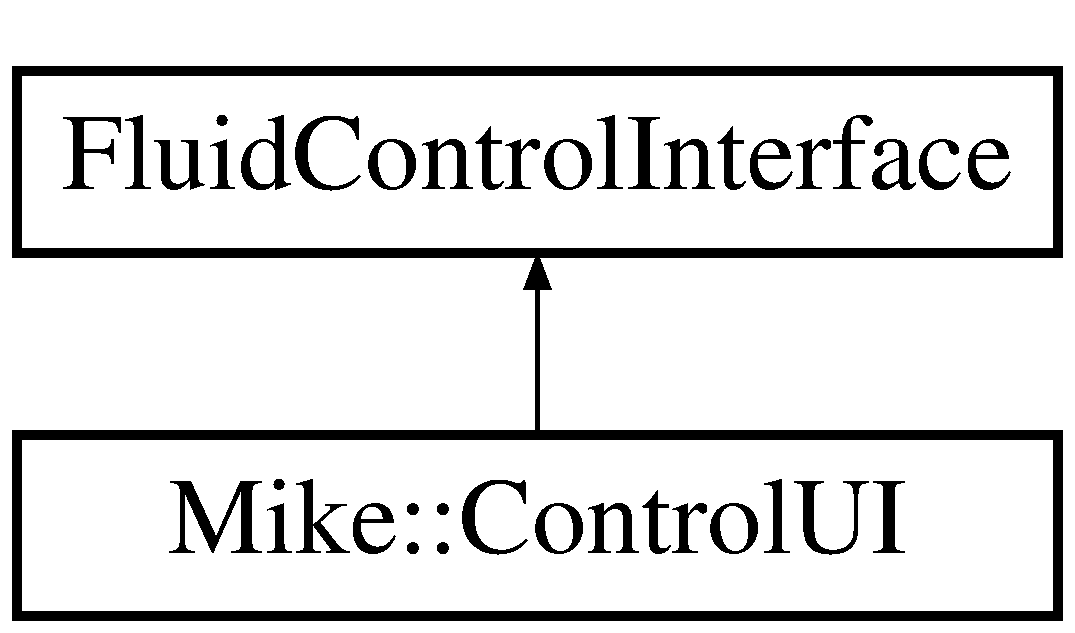
\includegraphics[height=2.000000cm]{class_mike_1_1_control_u_i}
\end{center}
\end{figure}
\subsection*{Public Member Functions}
\begin{DoxyCompactItemize}
\item 
\hyperlink{class_mike_1_1_control_u_i_ab62701989c636033cd6756c332a43513}{Control\+UI} ()
\item 
\hyperlink{class_mike_1_1_control_u_i_af2e1bde555402a1035d7f8e2b1525b50}{$\sim$\+Control\+UI} ()
\item 
bool \hyperlink{class_mike_1_1_control_u_i_afb11a656dc093a18fd3f12f9b9709418}{events\+Waiting} ()
\item 
\hyperlink{struct_mike_1_1_control_u_i_event}{Control\+U\+I\+Event} \hyperlink{class_mike_1_1_control_u_i_ae5bb9cf35b75c37381573ce7469504f1}{get\+Next\+Event} ()
\end{DoxyCompactItemize}
\subsection*{Private Member Functions}
\begin{DoxyCompactItemize}
\item 
void \hyperlink{class_mike_1_1_control_u_i_abcc1603903c8fd267ca9ce1a559266a9}{add\+User\+Event} (\hyperlink{namespace_mike_ab036b30a5fb5ef61314086e0c2c5ca6a}{Control\+U\+I\+Button} btn\+Pressed\+By\+User)
\end{DoxyCompactItemize}
\subsection*{Static Private Member Functions}
\begin{DoxyCompactItemize}
\item 
static void \hyperlink{class_mike_1_1_control_u_i_aaf2f6fc2cf93202867a797cf7bb6cc3e}{S\+T\+A\+R\+T\+L\+O\+O\+Pfltk\+K\+Btncallback} (Fl\+\_\+\+Widget $\ast$w, void $\ast$pointer\+Passed)
\item 
static void \hyperlink{class_mike_1_1_control_u_i_af3a7231a14cd112112e3e1c71e10baa1}{S\+T\+O\+P\+L\+O\+O\+Pfltk\+K\+Btncallback} (Fl\+\_\+\+Widget $\ast$w, void $\ast$pointer\+Passed)
\item 
static void \hyperlink{class_mike_1_1_control_u_i_ae37ce9f312e0f906a4847d6690927e27}{P\+O\+S\+I\+T\+I\+O\+N\+S1fltk\+K\+Btncallback} (Fl\+\_\+\+Widget $\ast$w, void $\ast$pointer\+Passed)
\end{DoxyCompactItemize}
\subsection*{Private Attributes}
\begin{DoxyCompactItemize}
\item 
std\+::queue$<$ \hyperlink{struct_mike_1_1_control_u_i_event}{Control\+U\+I\+Event} $>$ \hyperlink{class_mike_1_1_control_u_i_ae46585298dfd8ddb97a4d64168cc39e1}{m\+Event\+Queue}
\end{DoxyCompactItemize}
\subsection*{Friends}
\begin{DoxyCompactItemize}
\item 
class \hyperlink{class_mike_1_1_control_u_i_a9adf7c444a8611024541177662d4716a}{Control}
\end{DoxyCompactItemize}
\subsection*{Additional Inherited Members}


\subsection{Detailed Description}
Creates a window with buttons for controlling the \hyperlink{class_mike_1_1_control}{Control} class. Use F\+L\+U\+ID software to design/modify the window described in \hyperlink{_fluid_control_interface_8h}{Fluid\+Control\+Interface.\+h} -\/ this class inherits from it. 

\subsection{Constructor \& Destructor Documentation}
\mbox{\Hypertarget{class_mike_1_1_control_u_i_ab62701989c636033cd6756c332a43513}\label{class_mike_1_1_control_u_i_ab62701989c636033cd6756c332a43513}} 
\index{Mike\+::\+Control\+UI@{Mike\+::\+Control\+UI}!Control\+UI@{Control\+UI}}
\index{Control\+UI@{Control\+UI}!Mike\+::\+Control\+UI@{Mike\+::\+Control\+UI}}
\subsubsection{\texorpdfstring{Control\+U\+I()}{ControlUI()}}
{\footnotesize\ttfamily Mike\+::\+Control\+U\+I\+::\+Control\+UI (\begin{DoxyParamCaption}{ }\end{DoxyParamCaption})}

Constructor. Displays the window by default. Assign callbacks here. \mbox{\Hypertarget{class_mike_1_1_control_u_i_af2e1bde555402a1035d7f8e2b1525b50}\label{class_mike_1_1_control_u_i_af2e1bde555402a1035d7f8e2b1525b50}} 
\index{Mike\+::\+Control\+UI@{Mike\+::\+Control\+UI}!````~Control\+UI@{$\sim$\+Control\+UI}}
\index{````~Control\+UI@{$\sim$\+Control\+UI}!Mike\+::\+Control\+UI@{Mike\+::\+Control\+UI}}
\subsubsection{\texorpdfstring{$\sim$\+Control\+U\+I()}{~ControlUI()}}
{\footnotesize\ttfamily Mike\+::\+Control\+U\+I\+::$\sim$\+Control\+UI (\begin{DoxyParamCaption}{ }\end{DoxyParamCaption})}



\subsection{Member Function Documentation}
\mbox{\Hypertarget{class_mike_1_1_control_u_i_abcc1603903c8fd267ca9ce1a559266a9}\label{class_mike_1_1_control_u_i_abcc1603903c8fd267ca9ce1a559266a9}} 
\index{Mike\+::\+Control\+UI@{Mike\+::\+Control\+UI}!add\+User\+Event@{add\+User\+Event}}
\index{add\+User\+Event@{add\+User\+Event}!Mike\+::\+Control\+UI@{Mike\+::\+Control\+UI}}
\subsubsection{\texorpdfstring{add\+User\+Event()}{addUserEvent()}}
{\footnotesize\ttfamily void Mike\+::\+Control\+U\+I\+::add\+User\+Event (\begin{DoxyParamCaption}\item[{\hyperlink{namespace_mike_ab036b30a5fb5ef61314086e0c2c5ca6a}{Control\+U\+I\+Button}}]{btn\+Pressed\+By\+User }\end{DoxyParamCaption})\hspace{0.3cm}{\ttfamily [private]}}

Used by F\+L\+TK static callbacks to add buttons pressed by user to m\+Event\+Queue \mbox{\Hypertarget{class_mike_1_1_control_u_i_afb11a656dc093a18fd3f12f9b9709418}\label{class_mike_1_1_control_u_i_afb11a656dc093a18fd3f12f9b9709418}} 
\index{Mike\+::\+Control\+UI@{Mike\+::\+Control\+UI}!events\+Waiting@{events\+Waiting}}
\index{events\+Waiting@{events\+Waiting}!Mike\+::\+Control\+UI@{Mike\+::\+Control\+UI}}
\subsubsection{\texorpdfstring{events\+Waiting()}{eventsWaiting()}}
{\footnotesize\ttfamily bool Mike\+::\+Control\+U\+I\+::events\+Waiting (\begin{DoxyParamCaption}{ }\end{DoxyParamCaption})\hspace{0.3cm}{\ttfamily [inline]}}

Returns true if there are any callbacks in the queue (m\+Event\+Queue) that are waiting to be handled. False if queue is empty. \mbox{\Hypertarget{class_mike_1_1_control_u_i_ae5bb9cf35b75c37381573ce7469504f1}\label{class_mike_1_1_control_u_i_ae5bb9cf35b75c37381573ce7469504f1}} 
\index{Mike\+::\+Control\+UI@{Mike\+::\+Control\+UI}!get\+Next\+Event@{get\+Next\+Event}}
\index{get\+Next\+Event@{get\+Next\+Event}!Mike\+::\+Control\+UI@{Mike\+::\+Control\+UI}}
\subsubsection{\texorpdfstring{get\+Next\+Event()}{getNextEvent()}}
{\footnotesize\ttfamily \hyperlink{struct_mike_1_1_control_u_i_event}{Control\+U\+I\+Event} Mike\+::\+Control\+U\+I\+::get\+Next\+Event (\begin{DoxyParamCaption}{ }\end{DoxyParamCaption})}

Not thread safe. Check that queue is not empty using \hyperlink{class_mike_1_1_control_u_i_afb11a656dc093a18fd3f12f9b9709418}{events\+Waiting()} before calling this. Returns the next event from the m\+Event\+Queue and removes that item from the queue. If this event is notprocessed by the caller then it is lost. Returns a dummy event with m\+Button\+Pressed = E\+M\+P\+TY if there are no elements in the queue and the caller decided to call this function without checkig for that. \mbox{\Hypertarget{class_mike_1_1_control_u_i_ae37ce9f312e0f906a4847d6690927e27}\label{class_mike_1_1_control_u_i_ae37ce9f312e0f906a4847d6690927e27}} 
\index{Mike\+::\+Control\+UI@{Mike\+::\+Control\+UI}!P\+O\+S\+I\+T\+I\+O\+N\+S1fltk\+K\+Btncallback@{P\+O\+S\+I\+T\+I\+O\+N\+S1fltk\+K\+Btncallback}}
\index{P\+O\+S\+I\+T\+I\+O\+N\+S1fltk\+K\+Btncallback@{P\+O\+S\+I\+T\+I\+O\+N\+S1fltk\+K\+Btncallback}!Mike\+::\+Control\+UI@{Mike\+::\+Control\+UI}}
\subsubsection{\texorpdfstring{P\+O\+S\+I\+T\+I\+O\+N\+S1fltk\+K\+Btncallback()}{POSITIONS1fltkKBtncallback()}}
{\footnotesize\ttfamily void Mike\+::\+Control\+U\+I\+::\+P\+O\+S\+I\+T\+I\+O\+N\+S1fltk\+K\+Btncallback (\begin{DoxyParamCaption}\item[{Fl\+\_\+\+Widget $\ast$}]{w,  }\item[{void $\ast$}]{pointer\+Passed }\end{DoxyParamCaption})\hspace{0.3cm}{\ttfamily [static]}, {\ttfamily [private]}}

F\+L\+TK callback for pressing Positions1 button \mbox{\Hypertarget{class_mike_1_1_control_u_i_aaf2f6fc2cf93202867a797cf7bb6cc3e}\label{class_mike_1_1_control_u_i_aaf2f6fc2cf93202867a797cf7bb6cc3e}} 
\index{Mike\+::\+Control\+UI@{Mike\+::\+Control\+UI}!S\+T\+A\+R\+T\+L\+O\+O\+Pfltk\+K\+Btncallback@{S\+T\+A\+R\+T\+L\+O\+O\+Pfltk\+K\+Btncallback}}
\index{S\+T\+A\+R\+T\+L\+O\+O\+Pfltk\+K\+Btncallback@{S\+T\+A\+R\+T\+L\+O\+O\+Pfltk\+K\+Btncallback}!Mike\+::\+Control\+UI@{Mike\+::\+Control\+UI}}
\subsubsection{\texorpdfstring{S\+T\+A\+R\+T\+L\+O\+O\+Pfltk\+K\+Btncallback()}{STARTLOOPfltkKBtncallback()}}
{\footnotesize\ttfamily void Mike\+::\+Control\+U\+I\+::\+S\+T\+A\+R\+T\+L\+O\+O\+Pfltk\+K\+Btncallback (\begin{DoxyParamCaption}\item[{Fl\+\_\+\+Widget $\ast$}]{w,  }\item[{void $\ast$}]{pointer\+Passed }\end{DoxyParamCaption})\hspace{0.3cm}{\ttfamily [static]}, {\ttfamily [private]}}

F\+L\+TK callback for pressing Start\+Loop button \mbox{\Hypertarget{class_mike_1_1_control_u_i_af3a7231a14cd112112e3e1c71e10baa1}\label{class_mike_1_1_control_u_i_af3a7231a14cd112112e3e1c71e10baa1}} 
\index{Mike\+::\+Control\+UI@{Mike\+::\+Control\+UI}!S\+T\+O\+P\+L\+O\+O\+Pfltk\+K\+Btncallback@{S\+T\+O\+P\+L\+O\+O\+Pfltk\+K\+Btncallback}}
\index{S\+T\+O\+P\+L\+O\+O\+Pfltk\+K\+Btncallback@{S\+T\+O\+P\+L\+O\+O\+Pfltk\+K\+Btncallback}!Mike\+::\+Control\+UI@{Mike\+::\+Control\+UI}}
\subsubsection{\texorpdfstring{S\+T\+O\+P\+L\+O\+O\+Pfltk\+K\+Btncallback()}{STOPLOOPfltkKBtncallback()}}
{\footnotesize\ttfamily void Mike\+::\+Control\+U\+I\+::\+S\+T\+O\+P\+L\+O\+O\+Pfltk\+K\+Btncallback (\begin{DoxyParamCaption}\item[{Fl\+\_\+\+Widget $\ast$}]{w,  }\item[{void $\ast$}]{pointer\+Passed }\end{DoxyParamCaption})\hspace{0.3cm}{\ttfamily [static]}, {\ttfamily [private]}}

F\+L\+TK callback for pressing Stop\+Loop button 

\subsection{Friends And Related Function Documentation}
\mbox{\Hypertarget{class_mike_1_1_control_u_i_a9adf7c444a8611024541177662d4716a}\label{class_mike_1_1_control_u_i_a9adf7c444a8611024541177662d4716a}} 
\index{Mike\+::\+Control\+UI@{Mike\+::\+Control\+UI}!Control@{Control}}
\index{Control@{Control}!Mike\+::\+Control\+UI@{Mike\+::\+Control\+UI}}
\subsubsection{\texorpdfstring{Control}{Control}}
{\footnotesize\ttfamily friend class \hyperlink{class_mike_1_1_control}{Control}\hspace{0.3cm}{\ttfamily [friend]}}



\subsection{Member Data Documentation}
\mbox{\Hypertarget{class_mike_1_1_control_u_i_ae46585298dfd8ddb97a4d64168cc39e1}\label{class_mike_1_1_control_u_i_ae46585298dfd8ddb97a4d64168cc39e1}} 
\index{Mike\+::\+Control\+UI@{Mike\+::\+Control\+UI}!m\+Event\+Queue@{m\+Event\+Queue}}
\index{m\+Event\+Queue@{m\+Event\+Queue}!Mike\+::\+Control\+UI@{Mike\+::\+Control\+UI}}
\subsubsection{\texorpdfstring{m\+Event\+Queue}{mEventQueue}}
{\footnotesize\ttfamily std\+::queue$<$\hyperlink{struct_mike_1_1_control_u_i_event}{Control\+U\+I\+Event}$>$ Mike\+::\+Control\+U\+I\+::m\+Event\+Queue\hspace{0.3cm}{\ttfamily [private]}}

Queue for handling callbacks. All callbacks are added to a queue. Use method bool \hyperlink{class_mike_1_1_control_u_i_afb11a656dc093a18fd3f12f9b9709418}{events\+Waiting()} to check if any button have been pressed. Use method get\+Next\+Event to get next callback and remove it from the queue 

The documentation for this class was generated from the following files\+:\begin{DoxyCompactItemize}
\item 
src/\+User\+Interfaces/\hyperlink{_control_u_i_8h}{Control\+U\+I.\+h}\item 
src/\+User\+Interfaces/\hyperlink{_control_u_i_8cpp}{Control\+U\+I.\+cpp}\end{DoxyCompactItemize}

\hypertarget{struct_mike_1_1_control_u_i_event}{}\section{Mike\+:\+:Control\+U\+I\+Event Struct Reference}
\label{struct_mike_1_1_control_u_i_event}\index{Mike\+::\+Control\+U\+I\+Event@{Mike\+::\+Control\+U\+I\+Event}}


{\ttfamily \#include $<$Control\+U\+I.\+h$>$}

\subsection*{Public Attributes}
\begin{DoxyCompactItemize}
\item 
\hyperlink{namespace_mike_ab036b30a5fb5ef61314086e0c2c5ca6a}{Control\+U\+I\+Button} \hyperlink{struct_mike_1_1_control_u_i_event_adf53b39417816ab95cd27ab7dec31707}{m\+Button\+Pressed}
\end{DoxyCompactItemize}


\subsection{Detailed Description}
Simple struct holding buttons/events pressed by user. Yes perhaps in this class it could be a simple enum instead -\/ but creating this for symmetry in other classes where additional parameters might need to be passed. 

\subsection{Member Data Documentation}
\mbox{\Hypertarget{struct_mike_1_1_control_u_i_event_adf53b39417816ab95cd27ab7dec31707}\label{struct_mike_1_1_control_u_i_event_adf53b39417816ab95cd27ab7dec31707}} 
\index{Mike\+::\+Control\+U\+I\+Event@{Mike\+::\+Control\+U\+I\+Event}!m\+Button\+Pressed@{m\+Button\+Pressed}}
\index{m\+Button\+Pressed@{m\+Button\+Pressed}!Mike\+::\+Control\+U\+I\+Event@{Mike\+::\+Control\+U\+I\+Event}}
\subsubsection{\texorpdfstring{m\+Button\+Pressed}{mButtonPressed}}
{\footnotesize\ttfamily \hyperlink{namespace_mike_ab036b30a5fb5ef61314086e0c2c5ca6a}{Control\+U\+I\+Button} Mike\+::\+Control\+U\+I\+Event\+::m\+Button\+Pressed}



The documentation for this struct was generated from the following file\+:\begin{DoxyCompactItemize}
\item 
src/\+User\+Interfaces/\hyperlink{_control_u_i_8h}{Control\+U\+I.\+h}\end{DoxyCompactItemize}

\hypertarget{class_mike_1_1_data}{}\section{Mike\+:\+:Data Class Reference}
\label{class_mike_1_1_data}\index{Mike\+::\+Data@{Mike\+::\+Data}}


{\ttfamily \#include $<$Data.\+h$>$}

\subsection*{Public Member Functions}
\begin{DoxyCompactItemize}
\item 
\hyperlink{class_mike_1_1_data_afb88d046472d9a49f9ea16d6773d9def}{Data} ()
\end{DoxyCompactItemize}
\subsection*{Private Types}
\begin{DoxyCompactItemize}
\item 
typedef \hyperlink{class_fluid_price_control_u_i}{Fluid\+Price\+Control\+UI} \hyperlink{class_mike_1_1_data_a7d4ea849326ce9098b521ebc12317b58}{Data\+UI}
\end{DoxyCompactItemize}
\subsection*{Private Attributes}
\begin{DoxyCompactItemize}
\item 
\hyperlink{class_mike_1_1_data_a7d4ea849326ce9098b521ebc12317b58}{Data\+UI} $\ast$ \hyperlink{class_mike_1_1_data_a615c7c93b1c7addbe8e888ddbed837a4}{data\+Control\+Window}
\end{DoxyCompactItemize}


\subsection{Detailed Description}
Class designed for handling market data. Connects to Interactive Brokers to pull live bid/ask prices. Contains Order\+Server(currently local dummy) which sends orders to the market and checks if they are filled. 

\subsection{Member Typedef Documentation}
\mbox{\Hypertarget{class_mike_1_1_data_a7d4ea849326ce9098b521ebc12317b58}\label{class_mike_1_1_data_a7d4ea849326ce9098b521ebc12317b58}} 
\index{Mike\+::\+Data@{Mike\+::\+Data}!Data\+UI@{Data\+UI}}
\index{Data\+UI@{Data\+UI}!Mike\+::\+Data@{Mike\+::\+Data}}
\subsubsection{\texorpdfstring{Data\+UI}{DataUI}}
{\footnotesize\ttfamily typedef \hyperlink{class_fluid_price_control_u_i}{Fluid\+Price\+Control\+UI} \hyperlink{class_mike_1_1_data_a7d4ea849326ce9098b521ebc12317b58}{Mike\+::\+Data\+::\+Data\+UI}\hspace{0.3cm}{\ttfamily [private]}}

Data\+UI is an F\+L\+TK window controlling the \hyperlink{class_mike_1_1_data}{Data} class 

\subsection{Constructor \& Destructor Documentation}
\mbox{\Hypertarget{class_mike_1_1_data_afb88d046472d9a49f9ea16d6773d9def}\label{class_mike_1_1_data_afb88d046472d9a49f9ea16d6773d9def}} 
\index{Mike\+::\+Data@{Mike\+::\+Data}!Data@{Data}}
\index{Data@{Data}!Mike\+::\+Data@{Mike\+::\+Data}}
\subsubsection{\texorpdfstring{Data()}{Data()}}
{\footnotesize\ttfamily Mike\+::\+Data\+::\+Data (\begin{DoxyParamCaption}{ }\end{DoxyParamCaption})}



\subsection{Member Data Documentation}
\mbox{\Hypertarget{class_mike_1_1_data_a615c7c93b1c7addbe8e888ddbed837a4}\label{class_mike_1_1_data_a615c7c93b1c7addbe8e888ddbed837a4}} 
\index{Mike\+::\+Data@{Mike\+::\+Data}!data\+Control\+Window@{data\+Control\+Window}}
\index{data\+Control\+Window@{data\+Control\+Window}!Mike\+::\+Data@{Mike\+::\+Data}}
\subsubsection{\texorpdfstring{data\+Control\+Window}{dataControlWindow}}
{\footnotesize\ttfamily \hyperlink{class_mike_1_1_data_a7d4ea849326ce9098b521ebc12317b58}{Data\+UI}$\ast$ Mike\+::\+Data\+::data\+Control\+Window\hspace{0.3cm}{\ttfamily [private]}}

Data\+UI is a User Interface Window used to control everything associated with market price data. This is designed to grow. Market price data can be either pulled from Interactive Brokers using Jan Boonen\textquotesingle{}s library or it can be switched to \textquotesingle{}manual\textquotesingle{} to explore behaviour of algos. 

The documentation for this class was generated from the following files\+:\begin{DoxyCompactItemize}
\item 
src/\hyperlink{_data_8h}{Data.\+h}\item 
src/\hyperlink{_data_8cpp}{Data.\+cpp}\end{DoxyCompactItemize}

\hypertarget{class_mike_1_1_data_u_i}{}\section{Mike\+:\+:Data\+UI Class Reference}
\label{class_mike_1_1_data_u_i}\index{Mike\+::\+Data\+UI@{Mike\+::\+Data\+UI}}


{\ttfamily \#include $<$Data.\+h$>$}

Inheritance diagram for Mike\+:\+:Data\+UI\+:\begin{figure}[H]
\begin{center}
\leavevmode
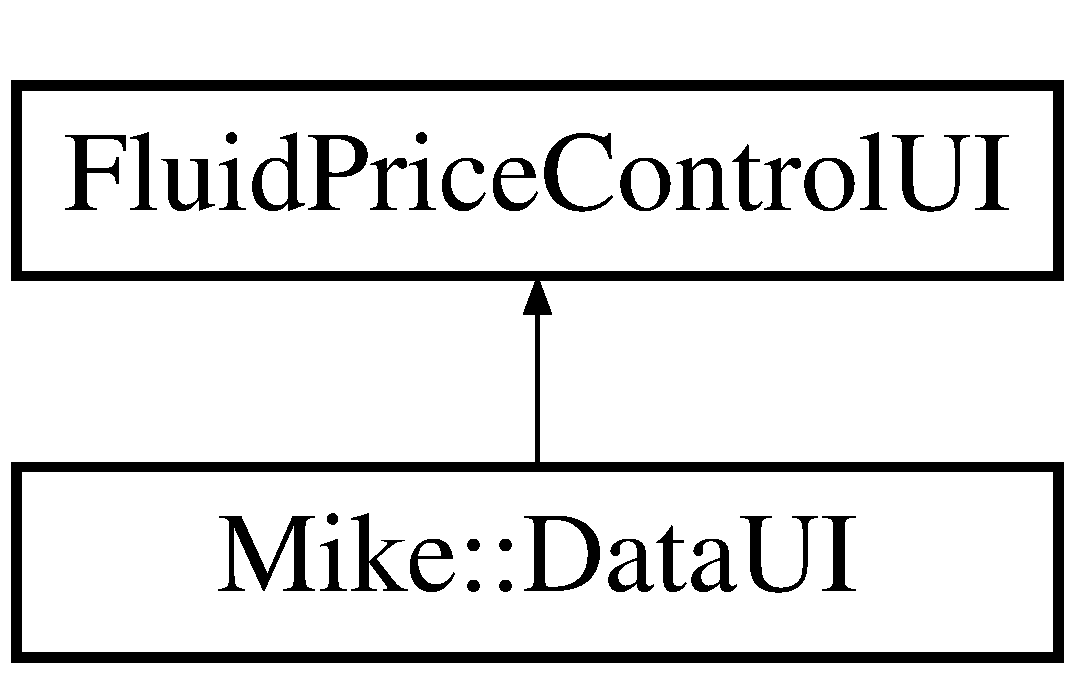
\includegraphics[height=2.000000cm]{class_mike_1_1_data_u_i}
\end{center}
\end{figure}
\subsection*{Public Member Functions}
\begin{DoxyCompactItemize}
\item 
\hyperlink{class_mike_1_1_data_u_i_ad2bc91f28168c7cc8bbcca47b54e59e8}{Data\+UI} ()
\end{DoxyCompactItemize}
\subsection*{Additional Inherited Members}


\subsection{Constructor \& Destructor Documentation}
\mbox{\Hypertarget{class_mike_1_1_data_u_i_ad2bc91f28168c7cc8bbcca47b54e59e8}\label{class_mike_1_1_data_u_i_ad2bc91f28168c7cc8bbcca47b54e59e8}} 
\index{Mike\+::\+Data\+UI@{Mike\+::\+Data\+UI}!Data\+UI@{Data\+UI}}
\index{Data\+UI@{Data\+UI}!Mike\+::\+Data\+UI@{Mike\+::\+Data\+UI}}
\subsubsection{\texorpdfstring{Data\+U\+I()}{DataUI()}}
{\footnotesize\ttfamily Mike\+::\+Data\+U\+I\+::\+Data\+UI (\begin{DoxyParamCaption}{ }\end{DoxyParamCaption})}



The documentation for this class was generated from the following files\+:\begin{DoxyCompactItemize}
\item 
src/\hyperlink{_data_8h}{Data.\+h}\item 
src/\hyperlink{_data_8cpp}{Data.\+cpp}\end{DoxyCompactItemize}

\hypertarget{struct_mike_1_1_data_u_i_event}{}\section{Mike\+:\+:Data\+U\+I\+Event Struct Reference}
\label{struct_mike_1_1_data_u_i_event}\index{Mike\+::\+Data\+U\+I\+Event@{Mike\+::\+Data\+U\+I\+Event}}


{\ttfamily \#include $<$Data.\+h$>$}

\subsection*{Public Attributes}
\begin{DoxyCompactItemize}
\item 
\hyperlink{namespace_mike_ac75044494e0b43141b5cefbcd63b7dde}{Data\+U\+I\+Button} \hyperlink{struct_mike_1_1_data_u_i_event_a0750106bd16c5494aa6402d16474b5b4}{m\+Button\+Pressed}
\end{DoxyCompactItemize}


\subsection{Detailed Description}
Simple struct holding buttons/events pressed by user. 

\subsection{Member Data Documentation}
\mbox{\Hypertarget{struct_mike_1_1_data_u_i_event_a0750106bd16c5494aa6402d16474b5b4}\label{struct_mike_1_1_data_u_i_event_a0750106bd16c5494aa6402d16474b5b4}} 
\index{Mike\+::\+Data\+U\+I\+Event@{Mike\+::\+Data\+U\+I\+Event}!m\+Button\+Pressed@{m\+Button\+Pressed}}
\index{m\+Button\+Pressed@{m\+Button\+Pressed}!Mike\+::\+Data\+U\+I\+Event@{Mike\+::\+Data\+U\+I\+Event}}
\subsubsection{\texorpdfstring{m\+Button\+Pressed}{mButtonPressed}}
{\footnotesize\ttfamily \hyperlink{namespace_mike_ac75044494e0b43141b5cefbcd63b7dde}{Data\+U\+I\+Button} Mike\+::\+Data\+U\+I\+Event\+::m\+Button\+Pressed}



The documentation for this struct was generated from the following file\+:\begin{DoxyCompactItemize}
\item 
src/\hyperlink{_data_8h}{Data.\+h}\end{DoxyCompactItemize}

\hypertarget{class_fluid_control_interface}{}\section{Fluid\+Control\+Interface Class Reference}
\label{class_fluid_control_interface}\index{Fluid\+Control\+Interface@{Fluid\+Control\+Interface}}


{\ttfamily \#include $<$Fluid\+Control\+Interface.\+h$>$}

Inheritance diagram for Fluid\+Control\+Interface\+:\begin{figure}[H]
\begin{center}
\leavevmode
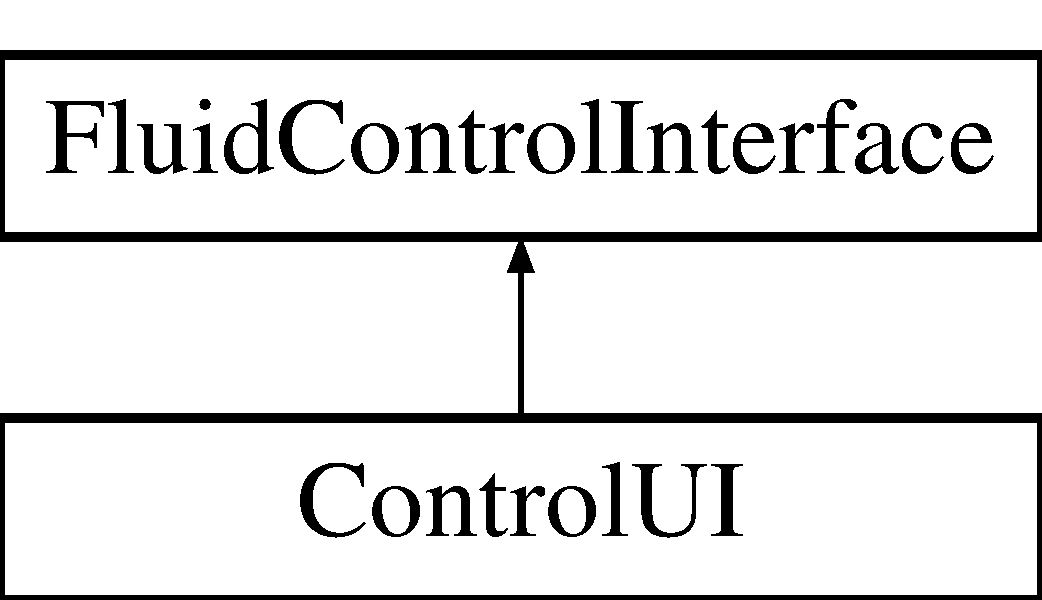
\includegraphics[height=2.000000cm]{class_fluid_control_interface}
\end{center}
\end{figure}
\subsection*{Public Member Functions}
\begin{DoxyCompactItemize}
\item 
\hyperlink{class_fluid_control_interface_a4cb172a43e95b2852f30807e9037a9d9}{Fluid\+Control\+Interface} ()
\end{DoxyCompactItemize}
\subsection*{Public Attributes}
\begin{DoxyCompactItemize}
\item 
Fl\+\_\+\+Double\+\_\+\+Window $\ast$ \hyperlink{class_fluid_control_interface_a94da1536108cd2bd24edefd8711ca510}{m\+Window}
\item 
Fl\+\_\+\+Box $\ast$ \hyperlink{class_fluid_control_interface_aad9032c096ff2feb1c72f534012282c9}{m\+Window\+Box}
\item 
Fl\+\_\+\+Button $\ast$ \hyperlink{class_fluid_control_interface_adc41c1528cbec12780e89140de2f8913}{m\+Btn\+Show\+Positions1}
\item 
Fl\+\_\+\+Button $\ast$ \hyperlink{class_fluid_control_interface_a3d74260a0b459e570427438dc5077db0}{m\+Btn\+Show\+Positions2}
\item 
Fl\+\_\+\+Button $\ast$ \hyperlink{class_fluid_control_interface_aedea42f561d246eb95442e13a88f8d23}{m\+Btn\+Show\+Positions3}
\item 
Fl\+\_\+\+Button $\ast$ \hyperlink{class_fluid_control_interface_a3827651fb223790ca880f23312266dde}{m\+Btn\+Show\+Positions4}
\item 
Fl\+\_\+\+Button $\ast$ \hyperlink{class_fluid_control_interface_a7d1930c1f10db9e39ce691f504b81387}{m\+Btn\+Start\+Loop}
\item 
Fl\+\_\+\+Button $\ast$ \hyperlink{class_fluid_control_interface_a885b36cf5c6e5ab82a2b6636579d840e}{m\+Btn\+Stop\+Loop}
\end{DoxyCompactItemize}


\subsection{Constructor \& Destructor Documentation}
\mbox{\Hypertarget{class_fluid_control_interface_a4cb172a43e95b2852f30807e9037a9d9}\label{class_fluid_control_interface_a4cb172a43e95b2852f30807e9037a9d9}} 
\index{Fluid\+Control\+Interface@{Fluid\+Control\+Interface}!Fluid\+Control\+Interface@{Fluid\+Control\+Interface}}
\index{Fluid\+Control\+Interface@{Fluid\+Control\+Interface}!Fluid\+Control\+Interface@{Fluid\+Control\+Interface}}
\subsubsection{\texorpdfstring{Fluid\+Control\+Interface()}{FluidControlInterface()}}
{\footnotesize\ttfamily Fluid\+Control\+Interface\+::\+Fluid\+Control\+Interface (\begin{DoxyParamCaption}{ }\end{DoxyParamCaption})}



\subsection{Member Data Documentation}
\mbox{\Hypertarget{class_fluid_control_interface_adc41c1528cbec12780e89140de2f8913}\label{class_fluid_control_interface_adc41c1528cbec12780e89140de2f8913}} 
\index{Fluid\+Control\+Interface@{Fluid\+Control\+Interface}!m\+Btn\+Show\+Positions1@{m\+Btn\+Show\+Positions1}}
\index{m\+Btn\+Show\+Positions1@{m\+Btn\+Show\+Positions1}!Fluid\+Control\+Interface@{Fluid\+Control\+Interface}}
\subsubsection{\texorpdfstring{m\+Btn\+Show\+Positions1}{mBtnShowPositions1}}
{\footnotesize\ttfamily Fl\+\_\+\+Button$\ast$ Fluid\+Control\+Interface\+::m\+Btn\+Show\+Positions1}

\mbox{\Hypertarget{class_fluid_control_interface_a3d74260a0b459e570427438dc5077db0}\label{class_fluid_control_interface_a3d74260a0b459e570427438dc5077db0}} 
\index{Fluid\+Control\+Interface@{Fluid\+Control\+Interface}!m\+Btn\+Show\+Positions2@{m\+Btn\+Show\+Positions2}}
\index{m\+Btn\+Show\+Positions2@{m\+Btn\+Show\+Positions2}!Fluid\+Control\+Interface@{Fluid\+Control\+Interface}}
\subsubsection{\texorpdfstring{m\+Btn\+Show\+Positions2}{mBtnShowPositions2}}
{\footnotesize\ttfamily Fl\+\_\+\+Button$\ast$ Fluid\+Control\+Interface\+::m\+Btn\+Show\+Positions2}

\mbox{\Hypertarget{class_fluid_control_interface_aedea42f561d246eb95442e13a88f8d23}\label{class_fluid_control_interface_aedea42f561d246eb95442e13a88f8d23}} 
\index{Fluid\+Control\+Interface@{Fluid\+Control\+Interface}!m\+Btn\+Show\+Positions3@{m\+Btn\+Show\+Positions3}}
\index{m\+Btn\+Show\+Positions3@{m\+Btn\+Show\+Positions3}!Fluid\+Control\+Interface@{Fluid\+Control\+Interface}}
\subsubsection{\texorpdfstring{m\+Btn\+Show\+Positions3}{mBtnShowPositions3}}
{\footnotesize\ttfamily Fl\+\_\+\+Button$\ast$ Fluid\+Control\+Interface\+::m\+Btn\+Show\+Positions3}

\mbox{\Hypertarget{class_fluid_control_interface_a3827651fb223790ca880f23312266dde}\label{class_fluid_control_interface_a3827651fb223790ca880f23312266dde}} 
\index{Fluid\+Control\+Interface@{Fluid\+Control\+Interface}!m\+Btn\+Show\+Positions4@{m\+Btn\+Show\+Positions4}}
\index{m\+Btn\+Show\+Positions4@{m\+Btn\+Show\+Positions4}!Fluid\+Control\+Interface@{Fluid\+Control\+Interface}}
\subsubsection{\texorpdfstring{m\+Btn\+Show\+Positions4}{mBtnShowPositions4}}
{\footnotesize\ttfamily Fl\+\_\+\+Button$\ast$ Fluid\+Control\+Interface\+::m\+Btn\+Show\+Positions4}

\mbox{\Hypertarget{class_fluid_control_interface_a7d1930c1f10db9e39ce691f504b81387}\label{class_fluid_control_interface_a7d1930c1f10db9e39ce691f504b81387}} 
\index{Fluid\+Control\+Interface@{Fluid\+Control\+Interface}!m\+Btn\+Start\+Loop@{m\+Btn\+Start\+Loop}}
\index{m\+Btn\+Start\+Loop@{m\+Btn\+Start\+Loop}!Fluid\+Control\+Interface@{Fluid\+Control\+Interface}}
\subsubsection{\texorpdfstring{m\+Btn\+Start\+Loop}{mBtnStartLoop}}
{\footnotesize\ttfamily Fl\+\_\+\+Button$\ast$ Fluid\+Control\+Interface\+::m\+Btn\+Start\+Loop}

\mbox{\Hypertarget{class_fluid_control_interface_a885b36cf5c6e5ab82a2b6636579d840e}\label{class_fluid_control_interface_a885b36cf5c6e5ab82a2b6636579d840e}} 
\index{Fluid\+Control\+Interface@{Fluid\+Control\+Interface}!m\+Btn\+Stop\+Loop@{m\+Btn\+Stop\+Loop}}
\index{m\+Btn\+Stop\+Loop@{m\+Btn\+Stop\+Loop}!Fluid\+Control\+Interface@{Fluid\+Control\+Interface}}
\subsubsection{\texorpdfstring{m\+Btn\+Stop\+Loop}{mBtnStopLoop}}
{\footnotesize\ttfamily Fl\+\_\+\+Button$\ast$ Fluid\+Control\+Interface\+::m\+Btn\+Stop\+Loop}

\mbox{\Hypertarget{class_fluid_control_interface_a94da1536108cd2bd24edefd8711ca510}\label{class_fluid_control_interface_a94da1536108cd2bd24edefd8711ca510}} 
\index{Fluid\+Control\+Interface@{Fluid\+Control\+Interface}!m\+Window@{m\+Window}}
\index{m\+Window@{m\+Window}!Fluid\+Control\+Interface@{Fluid\+Control\+Interface}}
\subsubsection{\texorpdfstring{m\+Window}{mWindow}}
{\footnotesize\ttfamily Fl\+\_\+\+Double\+\_\+\+Window$\ast$ Fluid\+Control\+Interface\+::m\+Window}

\mbox{\Hypertarget{class_fluid_control_interface_aad9032c096ff2feb1c72f534012282c9}\label{class_fluid_control_interface_aad9032c096ff2feb1c72f534012282c9}} 
\index{Fluid\+Control\+Interface@{Fluid\+Control\+Interface}!m\+Window\+Box@{m\+Window\+Box}}
\index{m\+Window\+Box@{m\+Window\+Box}!Fluid\+Control\+Interface@{Fluid\+Control\+Interface}}
\subsubsection{\texorpdfstring{m\+Window\+Box}{mWindowBox}}
{\footnotesize\ttfamily Fl\+\_\+\+Box$\ast$ Fluid\+Control\+Interface\+::m\+Window\+Box}



The documentation for this class was generated from the following files\+:\begin{DoxyCompactItemize}
\item 
src/\+F\+L\+U\+I\+D/\hyperlink{_fluid_control_interface_8h}{Fluid\+Control\+Interface.\+h}\item 
src/\+F\+L\+U\+I\+D/\hyperlink{_fluid_control_interface_8cxx}{Fluid\+Control\+Interface.\+cxx}\end{DoxyCompactItemize}

\hypertarget{class_fluid_interface}{}\section{Fluid\+Interface Class Reference}
\label{class_fluid_interface}\index{Fluid\+Interface@{Fluid\+Interface}}


{\ttfamily \#include $<$Fluid\+Interface.\+h$>$}

Inheritance diagram for Fluid\+Interface\+:\begin{figure}[H]
\begin{center}
\leavevmode
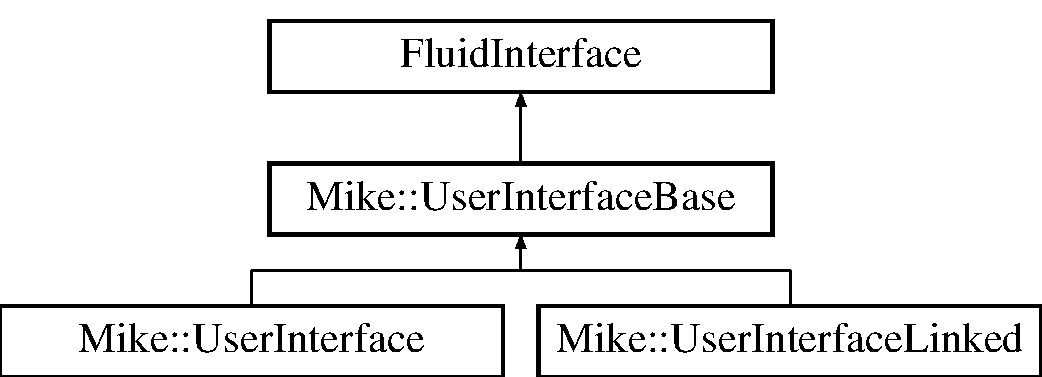
\includegraphics[height=3.000000cm]{class_fluid_interface}
\end{center}
\end{figure}
\subsection*{Public Member Functions}
\begin{DoxyCompactItemize}
\item 
\hyperlink{class_fluid_interface_a8d908e649929ac29ee7c7ea1d58972be}{Fluid\+Interface} ()
\end{DoxyCompactItemize}
\subsection*{Public Attributes}
\begin{DoxyCompactItemize}
\item 
Fl\+\_\+\+Double\+\_\+\+Window $\ast$ \hyperlink{class_fluid_interface_a460e32e78feb976474ee0735d0e9fb1c}{m\+\_\+window1}
\item 
Fl\+\_\+\+Value\+\_\+\+Input $\ast$ \hyperlink{class_fluid_interface_ad3602a1cc7b792c75382ea9499ab8dd7}{m\+\_\+curr\+\_\+ask}
\item 
Fl\+\_\+\+Value\+\_\+\+Input $\ast$ \hyperlink{class_fluid_interface_a81b5e83db29bcbfee9e6affed03befbf}{m\+\_\+top\+\_\+limit}
\item 
Fl\+\_\+\+Value\+\_\+\+Input $\ast$ \hyperlink{class_fluid_interface_abea73a05d352082acbecb7e16210708c}{m\+\_\+top\+\_\+profit}
\item 
Fl\+\_\+\+Table $\ast$ \hyperlink{class_fluid_interface_a18542e676efe12b02f8f942a9cec8a62}{m\+\_\+table}
\item 
Fl\+\_\+\+Value\+\_\+\+Input $\ast$ \hyperlink{class_fluid_interface_a510a2ac2cf61761833226823f434a72c}{m\+\_\+curr\+\_\+bid}
\item 
Fl\+\_\+\+Value\+\_\+\+Input $\ast$ \hyperlink{class_fluid_interface_a934958466791ab5e58dc419e83e841e9}{m\+\_\+bottom\+\_\+limit}
\item 
Fl\+\_\+\+Value\+\_\+\+Input $\ast$ \hyperlink{class_fluid_interface_ac19438e0f4c4e8578dc19924baa22757}{m\+\_\+bottom\+\_\+profit}
\item 
Fl\+\_\+\+Button $\ast$ \hyperlink{class_fluid_interface_aa022e70f1c8931e1e900dd02fcc0edb8}{m\+\_\+btn\+\_\+extra}
\item 
Fl\+\_\+\+Output $\ast$ \hyperlink{class_fluid_interface_a7527438818bbe46c24eaa4bf2937edd7}{m\+\_\+\+Tot\+Open\+Pos}
\item 
Fl\+\_\+\+Output $\ast$ \hyperlink{class_fluid_interface_aca2934bd9b472aa0abd681b401d619fa}{m\+\_\+\+Tot\+Open\+PL}
\item 
Fl\+\_\+\+Output $\ast$ \hyperlink{class_fluid_interface_ac0b9cbb054516b180ea22b1df083aaf6}{m\+\_\+\+Tot\+Closed\+PL}
\item 
Fl\+\_\+\+Output $\ast$ \hyperlink{class_fluid_interface_acb76315615db2a907ba49a8c0a8f24aa}{m\+\_\+\+Tot\+PL}
\item 
Fl\+\_\+\+Button $\ast$ \hyperlink{class_fluid_interface_aaaf08b63cd10cc8d3b247e4d24da6e5a}{m\+\_\+btn\+\_\+print\+Orders}
\item 
Fl\+\_\+\+Button $\ast$ \hyperlink{class_fluid_interface_a508b3c5a146b4275534b2c6881740282}{m\+\_\+btn\+\_\+check\+Fills}
\item 
Fl\+\_\+\+Button $\ast$ \hyperlink{class_fluid_interface_af62f75d2e5b156fe243becb5635f2bf3}{m\+\_\+btn\+\_\+print\+Pos}
\item 
Fl\+\_\+\+Value\+\_\+\+Input $\ast$ \hyperlink{class_fluid_interface_ae24f85770e0950a85ad3edf40bac3321}{m\+\_\+order\+\_\+size}
\item 
Fl\+\_\+\+Button $\ast$ \hyperlink{class_fluid_interface_a9173a1074dddfe66553518d7caa8f9d1}{m\+\_\+btn\+\_\+reset\+Ord\+Size}
\item 
Fl\+\_\+\+Button $\ast$ \hyperlink{class_fluid_interface_a974f975acf9f9be805e25908978d879b}{m\+\_\+btn\+\_\+\+Cancel\+All\+Orders}
\item 
Fl\+\_\+\+Output $\ast$ \hyperlink{class_fluid_interface_a6106c5c65a144e105a586e989250ffa3}{m\+\_\+\+Avg\+Pos\+Price}
\item 
Fl\+\_\+\+Button $\ast$ \hyperlink{class_fluid_interface_a479ef6af6e3c45db0f51a2b95a065672}{m\+\_\+btn\+\_\+\+Clear\+Positions}
\end{DoxyCompactItemize}


\subsection{Constructor \& Destructor Documentation}
\mbox{\Hypertarget{class_fluid_interface_a8d908e649929ac29ee7c7ea1d58972be}\label{class_fluid_interface_a8d908e649929ac29ee7c7ea1d58972be}} 
\index{Fluid\+Interface@{Fluid\+Interface}!Fluid\+Interface@{Fluid\+Interface}}
\index{Fluid\+Interface@{Fluid\+Interface}!Fluid\+Interface@{Fluid\+Interface}}
\subsubsection{\texorpdfstring{Fluid\+Interface()}{FluidInterface()}}
{\footnotesize\ttfamily Fluid\+Interface\+::\+Fluid\+Interface (\begin{DoxyParamCaption}{ }\end{DoxyParamCaption})}



\subsection{Member Data Documentation}
\mbox{\Hypertarget{class_fluid_interface_a6106c5c65a144e105a586e989250ffa3}\label{class_fluid_interface_a6106c5c65a144e105a586e989250ffa3}} 
\index{Fluid\+Interface@{Fluid\+Interface}!m\+\_\+\+Avg\+Pos\+Price@{m\+\_\+\+Avg\+Pos\+Price}}
\index{m\+\_\+\+Avg\+Pos\+Price@{m\+\_\+\+Avg\+Pos\+Price}!Fluid\+Interface@{Fluid\+Interface}}
\subsubsection{\texorpdfstring{m\+\_\+\+Avg\+Pos\+Price}{m\_AvgPosPrice}}
{\footnotesize\ttfamily Fl\+\_\+\+Output$\ast$ Fluid\+Interface\+::m\+\_\+\+Avg\+Pos\+Price}

\mbox{\Hypertarget{class_fluid_interface_a934958466791ab5e58dc419e83e841e9}\label{class_fluid_interface_a934958466791ab5e58dc419e83e841e9}} 
\index{Fluid\+Interface@{Fluid\+Interface}!m\+\_\+bottom\+\_\+limit@{m\+\_\+bottom\+\_\+limit}}
\index{m\+\_\+bottom\+\_\+limit@{m\+\_\+bottom\+\_\+limit}!Fluid\+Interface@{Fluid\+Interface}}
\subsubsection{\texorpdfstring{m\+\_\+bottom\+\_\+limit}{m\_bottom\_limit}}
{\footnotesize\ttfamily Fl\+\_\+\+Value\+\_\+\+Input$\ast$ Fluid\+Interface\+::m\+\_\+bottom\+\_\+limit}

\mbox{\Hypertarget{class_fluid_interface_ac19438e0f4c4e8578dc19924baa22757}\label{class_fluid_interface_ac19438e0f4c4e8578dc19924baa22757}} 
\index{Fluid\+Interface@{Fluid\+Interface}!m\+\_\+bottom\+\_\+profit@{m\+\_\+bottom\+\_\+profit}}
\index{m\+\_\+bottom\+\_\+profit@{m\+\_\+bottom\+\_\+profit}!Fluid\+Interface@{Fluid\+Interface}}
\subsubsection{\texorpdfstring{m\+\_\+bottom\+\_\+profit}{m\_bottom\_profit}}
{\footnotesize\ttfamily Fl\+\_\+\+Value\+\_\+\+Input$\ast$ Fluid\+Interface\+::m\+\_\+bottom\+\_\+profit}

\mbox{\Hypertarget{class_fluid_interface_a974f975acf9f9be805e25908978d879b}\label{class_fluid_interface_a974f975acf9f9be805e25908978d879b}} 
\index{Fluid\+Interface@{Fluid\+Interface}!m\+\_\+btn\+\_\+\+Cancel\+All\+Orders@{m\+\_\+btn\+\_\+\+Cancel\+All\+Orders}}
\index{m\+\_\+btn\+\_\+\+Cancel\+All\+Orders@{m\+\_\+btn\+\_\+\+Cancel\+All\+Orders}!Fluid\+Interface@{Fluid\+Interface}}
\subsubsection{\texorpdfstring{m\+\_\+btn\+\_\+\+Cancel\+All\+Orders}{m\_btn\_CancelAllOrders}}
{\footnotesize\ttfamily Fl\+\_\+\+Button$\ast$ Fluid\+Interface\+::m\+\_\+btn\+\_\+\+Cancel\+All\+Orders}

\mbox{\Hypertarget{class_fluid_interface_a508b3c5a146b4275534b2c6881740282}\label{class_fluid_interface_a508b3c5a146b4275534b2c6881740282}} 
\index{Fluid\+Interface@{Fluid\+Interface}!m\+\_\+btn\+\_\+check\+Fills@{m\+\_\+btn\+\_\+check\+Fills}}
\index{m\+\_\+btn\+\_\+check\+Fills@{m\+\_\+btn\+\_\+check\+Fills}!Fluid\+Interface@{Fluid\+Interface}}
\subsubsection{\texorpdfstring{m\+\_\+btn\+\_\+check\+Fills}{m\_btn\_checkFills}}
{\footnotesize\ttfamily Fl\+\_\+\+Button$\ast$ Fluid\+Interface\+::m\+\_\+btn\+\_\+check\+Fills}

\mbox{\Hypertarget{class_fluid_interface_a479ef6af6e3c45db0f51a2b95a065672}\label{class_fluid_interface_a479ef6af6e3c45db0f51a2b95a065672}} 
\index{Fluid\+Interface@{Fluid\+Interface}!m\+\_\+btn\+\_\+\+Clear\+Positions@{m\+\_\+btn\+\_\+\+Clear\+Positions}}
\index{m\+\_\+btn\+\_\+\+Clear\+Positions@{m\+\_\+btn\+\_\+\+Clear\+Positions}!Fluid\+Interface@{Fluid\+Interface}}
\subsubsection{\texorpdfstring{m\+\_\+btn\+\_\+\+Clear\+Positions}{m\_btn\_ClearPositions}}
{\footnotesize\ttfamily Fl\+\_\+\+Button$\ast$ Fluid\+Interface\+::m\+\_\+btn\+\_\+\+Clear\+Positions}

\mbox{\Hypertarget{class_fluid_interface_aa022e70f1c8931e1e900dd02fcc0edb8}\label{class_fluid_interface_aa022e70f1c8931e1e900dd02fcc0edb8}} 
\index{Fluid\+Interface@{Fluid\+Interface}!m\+\_\+btn\+\_\+extra@{m\+\_\+btn\+\_\+extra}}
\index{m\+\_\+btn\+\_\+extra@{m\+\_\+btn\+\_\+extra}!Fluid\+Interface@{Fluid\+Interface}}
\subsubsection{\texorpdfstring{m\+\_\+btn\+\_\+extra}{m\_btn\_extra}}
{\footnotesize\ttfamily Fl\+\_\+\+Button$\ast$ Fluid\+Interface\+::m\+\_\+btn\+\_\+extra}

\mbox{\Hypertarget{class_fluid_interface_aaaf08b63cd10cc8d3b247e4d24da6e5a}\label{class_fluid_interface_aaaf08b63cd10cc8d3b247e4d24da6e5a}} 
\index{Fluid\+Interface@{Fluid\+Interface}!m\+\_\+btn\+\_\+print\+Orders@{m\+\_\+btn\+\_\+print\+Orders}}
\index{m\+\_\+btn\+\_\+print\+Orders@{m\+\_\+btn\+\_\+print\+Orders}!Fluid\+Interface@{Fluid\+Interface}}
\subsubsection{\texorpdfstring{m\+\_\+btn\+\_\+print\+Orders}{m\_btn\_printOrders}}
{\footnotesize\ttfamily Fl\+\_\+\+Button$\ast$ Fluid\+Interface\+::m\+\_\+btn\+\_\+print\+Orders}

\mbox{\Hypertarget{class_fluid_interface_af62f75d2e5b156fe243becb5635f2bf3}\label{class_fluid_interface_af62f75d2e5b156fe243becb5635f2bf3}} 
\index{Fluid\+Interface@{Fluid\+Interface}!m\+\_\+btn\+\_\+print\+Pos@{m\+\_\+btn\+\_\+print\+Pos}}
\index{m\+\_\+btn\+\_\+print\+Pos@{m\+\_\+btn\+\_\+print\+Pos}!Fluid\+Interface@{Fluid\+Interface}}
\subsubsection{\texorpdfstring{m\+\_\+btn\+\_\+print\+Pos}{m\_btn\_printPos}}
{\footnotesize\ttfamily Fl\+\_\+\+Button$\ast$ Fluid\+Interface\+::m\+\_\+btn\+\_\+print\+Pos}

\mbox{\Hypertarget{class_fluid_interface_a9173a1074dddfe66553518d7caa8f9d1}\label{class_fluid_interface_a9173a1074dddfe66553518d7caa8f9d1}} 
\index{Fluid\+Interface@{Fluid\+Interface}!m\+\_\+btn\+\_\+reset\+Ord\+Size@{m\+\_\+btn\+\_\+reset\+Ord\+Size}}
\index{m\+\_\+btn\+\_\+reset\+Ord\+Size@{m\+\_\+btn\+\_\+reset\+Ord\+Size}!Fluid\+Interface@{Fluid\+Interface}}
\subsubsection{\texorpdfstring{m\+\_\+btn\+\_\+reset\+Ord\+Size}{m\_btn\_resetOrdSize}}
{\footnotesize\ttfamily Fl\+\_\+\+Button$\ast$ Fluid\+Interface\+::m\+\_\+btn\+\_\+reset\+Ord\+Size}

\mbox{\Hypertarget{class_fluid_interface_ad3602a1cc7b792c75382ea9499ab8dd7}\label{class_fluid_interface_ad3602a1cc7b792c75382ea9499ab8dd7}} 
\index{Fluid\+Interface@{Fluid\+Interface}!m\+\_\+curr\+\_\+ask@{m\+\_\+curr\+\_\+ask}}
\index{m\+\_\+curr\+\_\+ask@{m\+\_\+curr\+\_\+ask}!Fluid\+Interface@{Fluid\+Interface}}
\subsubsection{\texorpdfstring{m\+\_\+curr\+\_\+ask}{m\_curr\_ask}}
{\footnotesize\ttfamily Fl\+\_\+\+Value\+\_\+\+Input$\ast$ Fluid\+Interface\+::m\+\_\+curr\+\_\+ask}

\mbox{\Hypertarget{class_fluid_interface_a510a2ac2cf61761833226823f434a72c}\label{class_fluid_interface_a510a2ac2cf61761833226823f434a72c}} 
\index{Fluid\+Interface@{Fluid\+Interface}!m\+\_\+curr\+\_\+bid@{m\+\_\+curr\+\_\+bid}}
\index{m\+\_\+curr\+\_\+bid@{m\+\_\+curr\+\_\+bid}!Fluid\+Interface@{Fluid\+Interface}}
\subsubsection{\texorpdfstring{m\+\_\+curr\+\_\+bid}{m\_curr\_bid}}
{\footnotesize\ttfamily Fl\+\_\+\+Value\+\_\+\+Input$\ast$ Fluid\+Interface\+::m\+\_\+curr\+\_\+bid}

\mbox{\Hypertarget{class_fluid_interface_ae24f85770e0950a85ad3edf40bac3321}\label{class_fluid_interface_ae24f85770e0950a85ad3edf40bac3321}} 
\index{Fluid\+Interface@{Fluid\+Interface}!m\+\_\+order\+\_\+size@{m\+\_\+order\+\_\+size}}
\index{m\+\_\+order\+\_\+size@{m\+\_\+order\+\_\+size}!Fluid\+Interface@{Fluid\+Interface}}
\subsubsection{\texorpdfstring{m\+\_\+order\+\_\+size}{m\_order\_size}}
{\footnotesize\ttfamily Fl\+\_\+\+Value\+\_\+\+Input$\ast$ Fluid\+Interface\+::m\+\_\+order\+\_\+size}

\mbox{\Hypertarget{class_fluid_interface_a18542e676efe12b02f8f942a9cec8a62}\label{class_fluid_interface_a18542e676efe12b02f8f942a9cec8a62}} 
\index{Fluid\+Interface@{Fluid\+Interface}!m\+\_\+table@{m\+\_\+table}}
\index{m\+\_\+table@{m\+\_\+table}!Fluid\+Interface@{Fluid\+Interface}}
\subsubsection{\texorpdfstring{m\+\_\+table}{m\_table}}
{\footnotesize\ttfamily Fl\+\_\+\+Table$\ast$ Fluid\+Interface\+::m\+\_\+table}

\mbox{\Hypertarget{class_fluid_interface_a81b5e83db29bcbfee9e6affed03befbf}\label{class_fluid_interface_a81b5e83db29bcbfee9e6affed03befbf}} 
\index{Fluid\+Interface@{Fluid\+Interface}!m\+\_\+top\+\_\+limit@{m\+\_\+top\+\_\+limit}}
\index{m\+\_\+top\+\_\+limit@{m\+\_\+top\+\_\+limit}!Fluid\+Interface@{Fluid\+Interface}}
\subsubsection{\texorpdfstring{m\+\_\+top\+\_\+limit}{m\_top\_limit}}
{\footnotesize\ttfamily Fl\+\_\+\+Value\+\_\+\+Input$\ast$ Fluid\+Interface\+::m\+\_\+top\+\_\+limit}

\mbox{\Hypertarget{class_fluid_interface_abea73a05d352082acbecb7e16210708c}\label{class_fluid_interface_abea73a05d352082acbecb7e16210708c}} 
\index{Fluid\+Interface@{Fluid\+Interface}!m\+\_\+top\+\_\+profit@{m\+\_\+top\+\_\+profit}}
\index{m\+\_\+top\+\_\+profit@{m\+\_\+top\+\_\+profit}!Fluid\+Interface@{Fluid\+Interface}}
\subsubsection{\texorpdfstring{m\+\_\+top\+\_\+profit}{m\_top\_profit}}
{\footnotesize\ttfamily Fl\+\_\+\+Value\+\_\+\+Input$\ast$ Fluid\+Interface\+::m\+\_\+top\+\_\+profit}

\mbox{\Hypertarget{class_fluid_interface_ac0b9cbb054516b180ea22b1df083aaf6}\label{class_fluid_interface_ac0b9cbb054516b180ea22b1df083aaf6}} 
\index{Fluid\+Interface@{Fluid\+Interface}!m\+\_\+\+Tot\+Closed\+PL@{m\+\_\+\+Tot\+Closed\+PL}}
\index{m\+\_\+\+Tot\+Closed\+PL@{m\+\_\+\+Tot\+Closed\+PL}!Fluid\+Interface@{Fluid\+Interface}}
\subsubsection{\texorpdfstring{m\+\_\+\+Tot\+Closed\+PL}{m\_TotClosedPL}}
{\footnotesize\ttfamily Fl\+\_\+\+Output$\ast$ Fluid\+Interface\+::m\+\_\+\+Tot\+Closed\+PL}

\mbox{\Hypertarget{class_fluid_interface_aca2934bd9b472aa0abd681b401d619fa}\label{class_fluid_interface_aca2934bd9b472aa0abd681b401d619fa}} 
\index{Fluid\+Interface@{Fluid\+Interface}!m\+\_\+\+Tot\+Open\+PL@{m\+\_\+\+Tot\+Open\+PL}}
\index{m\+\_\+\+Tot\+Open\+PL@{m\+\_\+\+Tot\+Open\+PL}!Fluid\+Interface@{Fluid\+Interface}}
\subsubsection{\texorpdfstring{m\+\_\+\+Tot\+Open\+PL}{m\_TotOpenPL}}
{\footnotesize\ttfamily Fl\+\_\+\+Output$\ast$ Fluid\+Interface\+::m\+\_\+\+Tot\+Open\+PL}

\mbox{\Hypertarget{class_fluid_interface_a7527438818bbe46c24eaa4bf2937edd7}\label{class_fluid_interface_a7527438818bbe46c24eaa4bf2937edd7}} 
\index{Fluid\+Interface@{Fluid\+Interface}!m\+\_\+\+Tot\+Open\+Pos@{m\+\_\+\+Tot\+Open\+Pos}}
\index{m\+\_\+\+Tot\+Open\+Pos@{m\+\_\+\+Tot\+Open\+Pos}!Fluid\+Interface@{Fluid\+Interface}}
\subsubsection{\texorpdfstring{m\+\_\+\+Tot\+Open\+Pos}{m\_TotOpenPos}}
{\footnotesize\ttfamily Fl\+\_\+\+Output$\ast$ Fluid\+Interface\+::m\+\_\+\+Tot\+Open\+Pos}

\mbox{\Hypertarget{class_fluid_interface_acb76315615db2a907ba49a8c0a8f24aa}\label{class_fluid_interface_acb76315615db2a907ba49a8c0a8f24aa}} 
\index{Fluid\+Interface@{Fluid\+Interface}!m\+\_\+\+Tot\+PL@{m\+\_\+\+Tot\+PL}}
\index{m\+\_\+\+Tot\+PL@{m\+\_\+\+Tot\+PL}!Fluid\+Interface@{Fluid\+Interface}}
\subsubsection{\texorpdfstring{m\+\_\+\+Tot\+PL}{m\_TotPL}}
{\footnotesize\ttfamily Fl\+\_\+\+Output$\ast$ Fluid\+Interface\+::m\+\_\+\+Tot\+PL}

\mbox{\Hypertarget{class_fluid_interface_a460e32e78feb976474ee0735d0e9fb1c}\label{class_fluid_interface_a460e32e78feb976474ee0735d0e9fb1c}} 
\index{Fluid\+Interface@{Fluid\+Interface}!m\+\_\+window1@{m\+\_\+window1}}
\index{m\+\_\+window1@{m\+\_\+window1}!Fluid\+Interface@{Fluid\+Interface}}
\subsubsection{\texorpdfstring{m\+\_\+window1}{m\_window1}}
{\footnotesize\ttfamily Fl\+\_\+\+Double\+\_\+\+Window$\ast$ Fluid\+Interface\+::m\+\_\+window1}



The documentation for this class was generated from the following files\+:\begin{DoxyCompactItemize}
\item 
src/\+F\+L\+U\+I\+D/\hyperlink{_fluid_interface_8h}{Fluid\+Interface.\+h}\item 
src/\+F\+L\+U\+I\+D/\hyperlink{_fluid_interface_8cxx}{Fluid\+Interface.\+cxx}\end{DoxyCompactItemize}

\hypertarget{class_fluid_price_control_u_i}{}\section{Fluid\+Price\+Control\+UI Class Reference}
\label{class_fluid_price_control_u_i}\index{Fluid\+Price\+Control\+UI@{Fluid\+Price\+Control\+UI}}


{\ttfamily \#include $<$Fluid\+Price\+Control.\+h$>$}

\subsection*{Public Member Functions}
\begin{DoxyCompactItemize}
\item 
\hyperlink{class_fluid_price_control_u_i_a2cda3cd2bdafd0550ffd992166db9f9b}{Fluid\+Price\+Control\+UI} ()
\end{DoxyCompactItemize}
\subsection*{Public Attributes}
\begin{DoxyCompactItemize}
\item 
Fl\+\_\+\+Double\+\_\+\+Window $\ast$ \hyperlink{class_fluid_price_control_u_i_a65c8356043b3a182a177cf4a52317124}{m\+\_\+window1}
\item 
Fl\+\_\+\+Button $\ast$ \hyperlink{class_fluid_price_control_u_i_a17dcc8d29c4170578c8305d0bbce0f89}{m\+\_\+btn\+Up}
\item 
Fl\+\_\+\+Button $\ast$ \hyperlink{class_fluid_price_control_u_i_a98213f3a52dd6c6b700f5a20f1cfa7ab}{m\+\_\+btn\+Down}
\item 
Fl\+\_\+\+Output $\ast$ \hyperlink{class_fluid_price_control_u_i_afcc19c4bc7bc7295854861d2f667f457}{m\+\_\+\+Bid\+Display}
\item 
Fl\+\_\+\+Output $\ast$ \hyperlink{class_fluid_price_control_u_i_a68a7585dc66f65459fa6c38c086299f8}{m\+\_\+\+Ask\+Display}
\item 
Fl\+\_\+\+Value\+\_\+\+Slider $\ast$ \hyperlink{class_fluid_price_control_u_i_ad57bb65dd4c67780a86158e5d2ac7b90}{m\+\_\+slider1}
\item 
Fl\+\_\+\+Button $\ast$ \hyperlink{class_fluid_price_control_u_i_a0f591e3a87e7a68d05d1b17625d7de87}{m\+\_\+btn\+Print}
\item 
Fl\+\_\+\+Button $\ast$ \hyperlink{class_fluid_price_control_u_i_a6a6870f04d6e93c70975e8dbc463c8eb}{m\+\_\+btn\+Live\+Data\+Console\+Print}
\item 
Fl\+\_\+\+Button $\ast$ \hyperlink{class_fluid_price_control_u_i_a298e80045e3c1ea8cabbc21b0b3138ca}{m\+\_\+btn\+Connect\+Live\+Data}
\item 
Fl\+\_\+\+Button $\ast$ \hyperlink{class_fluid_price_control_u_i_a41892b034300821670f3e585bdd191a3}{m\+\_\+btn\+Start\+Loop}
\item 
Fl\+\_\+\+Button $\ast$ \hyperlink{class_fluid_price_control_u_i_ad94515ca4f97533e76a67e04bf4411e4}{m\+\_\+btn\+Experiment}
\end{DoxyCompactItemize}


\subsection{Constructor \& Destructor Documentation}
\mbox{\Hypertarget{class_fluid_price_control_u_i_a2cda3cd2bdafd0550ffd992166db9f9b}\label{class_fluid_price_control_u_i_a2cda3cd2bdafd0550ffd992166db9f9b}} 
\index{Fluid\+Price\+Control\+UI@{Fluid\+Price\+Control\+UI}!Fluid\+Price\+Control\+UI@{Fluid\+Price\+Control\+UI}}
\index{Fluid\+Price\+Control\+UI@{Fluid\+Price\+Control\+UI}!Fluid\+Price\+Control\+UI@{Fluid\+Price\+Control\+UI}}
\subsubsection{\texorpdfstring{Fluid\+Price\+Control\+U\+I()}{FluidPriceControlUI()}}
{\footnotesize\ttfamily Fluid\+Price\+Control\+U\+I\+::\+Fluid\+Price\+Control\+UI (\begin{DoxyParamCaption}{ }\end{DoxyParamCaption})}



\subsection{Member Data Documentation}
\mbox{\Hypertarget{class_fluid_price_control_u_i_a68a7585dc66f65459fa6c38c086299f8}\label{class_fluid_price_control_u_i_a68a7585dc66f65459fa6c38c086299f8}} 
\index{Fluid\+Price\+Control\+UI@{Fluid\+Price\+Control\+UI}!m\+\_\+\+Ask\+Display@{m\+\_\+\+Ask\+Display}}
\index{m\+\_\+\+Ask\+Display@{m\+\_\+\+Ask\+Display}!Fluid\+Price\+Control\+UI@{Fluid\+Price\+Control\+UI}}
\subsubsection{\texorpdfstring{m\+\_\+\+Ask\+Display}{m\_AskDisplay}}
{\footnotesize\ttfamily Fl\+\_\+\+Output$\ast$ Fluid\+Price\+Control\+U\+I\+::m\+\_\+\+Ask\+Display}

\mbox{\Hypertarget{class_fluid_price_control_u_i_afcc19c4bc7bc7295854861d2f667f457}\label{class_fluid_price_control_u_i_afcc19c4bc7bc7295854861d2f667f457}} 
\index{Fluid\+Price\+Control\+UI@{Fluid\+Price\+Control\+UI}!m\+\_\+\+Bid\+Display@{m\+\_\+\+Bid\+Display}}
\index{m\+\_\+\+Bid\+Display@{m\+\_\+\+Bid\+Display}!Fluid\+Price\+Control\+UI@{Fluid\+Price\+Control\+UI}}
\subsubsection{\texorpdfstring{m\+\_\+\+Bid\+Display}{m\_BidDisplay}}
{\footnotesize\ttfamily Fl\+\_\+\+Output$\ast$ Fluid\+Price\+Control\+U\+I\+::m\+\_\+\+Bid\+Display}

\mbox{\Hypertarget{class_fluid_price_control_u_i_a298e80045e3c1ea8cabbc21b0b3138ca}\label{class_fluid_price_control_u_i_a298e80045e3c1ea8cabbc21b0b3138ca}} 
\index{Fluid\+Price\+Control\+UI@{Fluid\+Price\+Control\+UI}!m\+\_\+btn\+Connect\+Live\+Data@{m\+\_\+btn\+Connect\+Live\+Data}}
\index{m\+\_\+btn\+Connect\+Live\+Data@{m\+\_\+btn\+Connect\+Live\+Data}!Fluid\+Price\+Control\+UI@{Fluid\+Price\+Control\+UI}}
\subsubsection{\texorpdfstring{m\+\_\+btn\+Connect\+Live\+Data}{m\_btnConnectLiveData}}
{\footnotesize\ttfamily Fl\+\_\+\+Button$\ast$ Fluid\+Price\+Control\+U\+I\+::m\+\_\+btn\+Connect\+Live\+Data}

\mbox{\Hypertarget{class_fluid_price_control_u_i_a98213f3a52dd6c6b700f5a20f1cfa7ab}\label{class_fluid_price_control_u_i_a98213f3a52dd6c6b700f5a20f1cfa7ab}} 
\index{Fluid\+Price\+Control\+UI@{Fluid\+Price\+Control\+UI}!m\+\_\+btn\+Down@{m\+\_\+btn\+Down}}
\index{m\+\_\+btn\+Down@{m\+\_\+btn\+Down}!Fluid\+Price\+Control\+UI@{Fluid\+Price\+Control\+UI}}
\subsubsection{\texorpdfstring{m\+\_\+btn\+Down}{m\_btnDown}}
{\footnotesize\ttfamily Fl\+\_\+\+Button$\ast$ Fluid\+Price\+Control\+U\+I\+::m\+\_\+btn\+Down}

\mbox{\Hypertarget{class_fluid_price_control_u_i_ad94515ca4f97533e76a67e04bf4411e4}\label{class_fluid_price_control_u_i_ad94515ca4f97533e76a67e04bf4411e4}} 
\index{Fluid\+Price\+Control\+UI@{Fluid\+Price\+Control\+UI}!m\+\_\+btn\+Experiment@{m\+\_\+btn\+Experiment}}
\index{m\+\_\+btn\+Experiment@{m\+\_\+btn\+Experiment}!Fluid\+Price\+Control\+UI@{Fluid\+Price\+Control\+UI}}
\subsubsection{\texorpdfstring{m\+\_\+btn\+Experiment}{m\_btnExperiment}}
{\footnotesize\ttfamily Fl\+\_\+\+Button$\ast$ Fluid\+Price\+Control\+U\+I\+::m\+\_\+btn\+Experiment}

\mbox{\Hypertarget{class_fluid_price_control_u_i_a6a6870f04d6e93c70975e8dbc463c8eb}\label{class_fluid_price_control_u_i_a6a6870f04d6e93c70975e8dbc463c8eb}} 
\index{Fluid\+Price\+Control\+UI@{Fluid\+Price\+Control\+UI}!m\+\_\+btn\+Live\+Data\+Console\+Print@{m\+\_\+btn\+Live\+Data\+Console\+Print}}
\index{m\+\_\+btn\+Live\+Data\+Console\+Print@{m\+\_\+btn\+Live\+Data\+Console\+Print}!Fluid\+Price\+Control\+UI@{Fluid\+Price\+Control\+UI}}
\subsubsection{\texorpdfstring{m\+\_\+btn\+Live\+Data\+Console\+Print}{m\_btnLiveDataConsolePrint}}
{\footnotesize\ttfamily Fl\+\_\+\+Button$\ast$ Fluid\+Price\+Control\+U\+I\+::m\+\_\+btn\+Live\+Data\+Console\+Print}

\mbox{\Hypertarget{class_fluid_price_control_u_i_a0f591e3a87e7a68d05d1b17625d7de87}\label{class_fluid_price_control_u_i_a0f591e3a87e7a68d05d1b17625d7de87}} 
\index{Fluid\+Price\+Control\+UI@{Fluid\+Price\+Control\+UI}!m\+\_\+btn\+Print@{m\+\_\+btn\+Print}}
\index{m\+\_\+btn\+Print@{m\+\_\+btn\+Print}!Fluid\+Price\+Control\+UI@{Fluid\+Price\+Control\+UI}}
\subsubsection{\texorpdfstring{m\+\_\+btn\+Print}{m\_btnPrint}}
{\footnotesize\ttfamily Fl\+\_\+\+Button$\ast$ Fluid\+Price\+Control\+U\+I\+::m\+\_\+btn\+Print}

\mbox{\Hypertarget{class_fluid_price_control_u_i_a41892b034300821670f3e585bdd191a3}\label{class_fluid_price_control_u_i_a41892b034300821670f3e585bdd191a3}} 
\index{Fluid\+Price\+Control\+UI@{Fluid\+Price\+Control\+UI}!m\+\_\+btn\+Start\+Loop@{m\+\_\+btn\+Start\+Loop}}
\index{m\+\_\+btn\+Start\+Loop@{m\+\_\+btn\+Start\+Loop}!Fluid\+Price\+Control\+UI@{Fluid\+Price\+Control\+UI}}
\subsubsection{\texorpdfstring{m\+\_\+btn\+Start\+Loop}{m\_btnStartLoop}}
{\footnotesize\ttfamily Fl\+\_\+\+Button$\ast$ Fluid\+Price\+Control\+U\+I\+::m\+\_\+btn\+Start\+Loop}

\mbox{\Hypertarget{class_fluid_price_control_u_i_a17dcc8d29c4170578c8305d0bbce0f89}\label{class_fluid_price_control_u_i_a17dcc8d29c4170578c8305d0bbce0f89}} 
\index{Fluid\+Price\+Control\+UI@{Fluid\+Price\+Control\+UI}!m\+\_\+btn\+Up@{m\+\_\+btn\+Up}}
\index{m\+\_\+btn\+Up@{m\+\_\+btn\+Up}!Fluid\+Price\+Control\+UI@{Fluid\+Price\+Control\+UI}}
\subsubsection{\texorpdfstring{m\+\_\+btn\+Up}{m\_btnUp}}
{\footnotesize\ttfamily Fl\+\_\+\+Button$\ast$ Fluid\+Price\+Control\+U\+I\+::m\+\_\+btn\+Up}

\mbox{\Hypertarget{class_fluid_price_control_u_i_ad57bb65dd4c67780a86158e5d2ac7b90}\label{class_fluid_price_control_u_i_ad57bb65dd4c67780a86158e5d2ac7b90}} 
\index{Fluid\+Price\+Control\+UI@{Fluid\+Price\+Control\+UI}!m\+\_\+slider1@{m\+\_\+slider1}}
\index{m\+\_\+slider1@{m\+\_\+slider1}!Fluid\+Price\+Control\+UI@{Fluid\+Price\+Control\+UI}}
\subsubsection{\texorpdfstring{m\+\_\+slider1}{m\_slider1}}
{\footnotesize\ttfamily Fl\+\_\+\+Value\+\_\+\+Slider$\ast$ Fluid\+Price\+Control\+U\+I\+::m\+\_\+slider1}

\mbox{\Hypertarget{class_fluid_price_control_u_i_a65c8356043b3a182a177cf4a52317124}\label{class_fluid_price_control_u_i_a65c8356043b3a182a177cf4a52317124}} 
\index{Fluid\+Price\+Control\+UI@{Fluid\+Price\+Control\+UI}!m\+\_\+window1@{m\+\_\+window1}}
\index{m\+\_\+window1@{m\+\_\+window1}!Fluid\+Price\+Control\+UI@{Fluid\+Price\+Control\+UI}}
\subsubsection{\texorpdfstring{m\+\_\+window1}{m\_window1}}
{\footnotesize\ttfamily Fl\+\_\+\+Double\+\_\+\+Window$\ast$ Fluid\+Price\+Control\+U\+I\+::m\+\_\+window1}



The documentation for this class was generated from the following files\+:\begin{DoxyCompactItemize}
\item 
F\+L\+U\+I\+D/\hyperlink{_fluid_price_control_8h}{Fluid\+Price\+Control.\+h}\item 
F\+L\+U\+I\+D/\hyperlink{_fluid_price_control_8cxx}{Fluid\+Price\+Control.\+cxx}\end{DoxyCompactItemize}

\hypertarget{class_mike_1_1_mike_order}{}\section{Mike\+:\+:Mike\+Order Class Reference}
\label{class_mike_1_1_mike_order}\index{Mike\+::\+Mike\+Order@{Mike\+::\+Mike\+Order}}


{\ttfamily \#include $<$Mike\+Enums.\+h$>$}

\subsection*{Public Attributes}
\begin{DoxyCompactItemize}
\item 
\hyperlink{namespace_mike_aa486aea8b1d0d07190982a311394e6cb}{Mike\+Order\+Type} \hyperlink{class_mike_1_1_mike_order_aa1acb12d7013d32b53c7aff946d2cbc8}{ordertype}
\item 
long \hyperlink{class_mike_1_1_mike_order_a4a74a640c2244eab7773339420d8c7a2}{assigned\+To\+Position} = 0
\item 
long \hyperlink{class_mike_1_1_mike_order_a134e751155f6f3c72c9cd600a9865d8f}{price} = 0
\item 
long \hyperlink{class_mike_1_1_mike_order_a77fd8fad7c335dce6f3543d640e2f223}{amount} = 0
\item 
long \hyperlink{class_mike_1_1_mike_order_a223c686cb5a0fe6e58926aa3d7e14381}{order\+Id}
\item 
bool \hyperlink{class_mike_1_1_mike_order_a835f8f61eb1eb1afcc409a5633612045}{is\+Filled} = false
\item 
bool \hyperlink{class_mike_1_1_mike_order_af03e7280847c51ac707e60727474b390}{partial\+Fill} = false
\item 
bool \hyperlink{class_mike_1_1_mike_order_a05565a668fb0ce47f2487c6de8a3fc38}{cancelled} = false
\end{DoxyCompactItemize}


\subsection{Member Data Documentation}
\mbox{\Hypertarget{class_mike_1_1_mike_order_a77fd8fad7c335dce6f3543d640e2f223}\label{class_mike_1_1_mike_order_a77fd8fad7c335dce6f3543d640e2f223}} 
\index{Mike\+::\+Mike\+Order@{Mike\+::\+Mike\+Order}!amount@{amount}}
\index{amount@{amount}!Mike\+::\+Mike\+Order@{Mike\+::\+Mike\+Order}}
\subsubsection{\texorpdfstring{amount}{amount}}
{\footnotesize\ttfamily long Mike\+::\+Mike\+Order\+::amount = 0}

\mbox{\Hypertarget{class_mike_1_1_mike_order_a4a74a640c2244eab7773339420d8c7a2}\label{class_mike_1_1_mike_order_a4a74a640c2244eab7773339420d8c7a2}} 
\index{Mike\+::\+Mike\+Order@{Mike\+::\+Mike\+Order}!assigned\+To\+Position@{assigned\+To\+Position}}
\index{assigned\+To\+Position@{assigned\+To\+Position}!Mike\+::\+Mike\+Order@{Mike\+::\+Mike\+Order}}
\subsubsection{\texorpdfstring{assigned\+To\+Position}{assignedToPosition}}
{\footnotesize\ttfamily long Mike\+::\+Mike\+Order\+::assigned\+To\+Position = 0}

\mbox{\Hypertarget{class_mike_1_1_mike_order_a05565a668fb0ce47f2487c6de8a3fc38}\label{class_mike_1_1_mike_order_a05565a668fb0ce47f2487c6de8a3fc38}} 
\index{Mike\+::\+Mike\+Order@{Mike\+::\+Mike\+Order}!cancelled@{cancelled}}
\index{cancelled@{cancelled}!Mike\+::\+Mike\+Order@{Mike\+::\+Mike\+Order}}
\subsubsection{\texorpdfstring{cancelled}{cancelled}}
{\footnotesize\ttfamily bool Mike\+::\+Mike\+Order\+::cancelled = false}

\mbox{\Hypertarget{class_mike_1_1_mike_order_a835f8f61eb1eb1afcc409a5633612045}\label{class_mike_1_1_mike_order_a835f8f61eb1eb1afcc409a5633612045}} 
\index{Mike\+::\+Mike\+Order@{Mike\+::\+Mike\+Order}!is\+Filled@{is\+Filled}}
\index{is\+Filled@{is\+Filled}!Mike\+::\+Mike\+Order@{Mike\+::\+Mike\+Order}}
\subsubsection{\texorpdfstring{is\+Filled}{isFilled}}
{\footnotesize\ttfamily bool Mike\+::\+Mike\+Order\+::is\+Filled = false}

\mbox{\Hypertarget{class_mike_1_1_mike_order_a223c686cb5a0fe6e58926aa3d7e14381}\label{class_mike_1_1_mike_order_a223c686cb5a0fe6e58926aa3d7e14381}} 
\index{Mike\+::\+Mike\+Order@{Mike\+::\+Mike\+Order}!order\+Id@{order\+Id}}
\index{order\+Id@{order\+Id}!Mike\+::\+Mike\+Order@{Mike\+::\+Mike\+Order}}
\subsubsection{\texorpdfstring{order\+Id}{orderId}}
{\footnotesize\ttfamily long Mike\+::\+Mike\+Order\+::order\+Id}

\mbox{\Hypertarget{class_mike_1_1_mike_order_aa1acb12d7013d32b53c7aff946d2cbc8}\label{class_mike_1_1_mike_order_aa1acb12d7013d32b53c7aff946d2cbc8}} 
\index{Mike\+::\+Mike\+Order@{Mike\+::\+Mike\+Order}!ordertype@{ordertype}}
\index{ordertype@{ordertype}!Mike\+::\+Mike\+Order@{Mike\+::\+Mike\+Order}}
\subsubsection{\texorpdfstring{ordertype}{ordertype}}
{\footnotesize\ttfamily \hyperlink{namespace_mike_aa486aea8b1d0d07190982a311394e6cb}{Mike\+Order\+Type} Mike\+::\+Mike\+Order\+::ordertype}

\mbox{\Hypertarget{class_mike_1_1_mike_order_af03e7280847c51ac707e60727474b390}\label{class_mike_1_1_mike_order_af03e7280847c51ac707e60727474b390}} 
\index{Mike\+::\+Mike\+Order@{Mike\+::\+Mike\+Order}!partial\+Fill@{partial\+Fill}}
\index{partial\+Fill@{partial\+Fill}!Mike\+::\+Mike\+Order@{Mike\+::\+Mike\+Order}}
\subsubsection{\texorpdfstring{partial\+Fill}{partialFill}}
{\footnotesize\ttfamily bool Mike\+::\+Mike\+Order\+::partial\+Fill = false}

\mbox{\Hypertarget{class_mike_1_1_mike_order_a134e751155f6f3c72c9cd600a9865d8f}\label{class_mike_1_1_mike_order_a134e751155f6f3c72c9cd600a9865d8f}} 
\index{Mike\+::\+Mike\+Order@{Mike\+::\+Mike\+Order}!price@{price}}
\index{price@{price}!Mike\+::\+Mike\+Order@{Mike\+::\+Mike\+Order}}
\subsubsection{\texorpdfstring{price}{price}}
{\footnotesize\ttfamily long Mike\+::\+Mike\+Order\+::price = 0}



The documentation for this class was generated from the following file\+:\begin{DoxyCompactItemize}
\item 
src/\hyperlink{_mike_enums_8h}{Mike\+Enums.\+h}\end{DoxyCompactItemize}

\hypertarget{class_mike_1_1_mike_orders_at_price}{}\section{Mike\+:\+:Mike\+Orders\+At\+Price Class Reference}
\label{class_mike_1_1_mike_orders_at_price}\index{Mike\+::\+Mike\+Orders\+At\+Price@{Mike\+::\+Mike\+Orders\+At\+Price}}


{\ttfamily \#include $<$Mike\+Enums.\+h$>$}

\subsection*{Public Member Functions}
\begin{DoxyCompactItemize}
\item 
void \hyperlink{class_mike_1_1_mike_orders_at_price_a75b42dff63234fb5b8a2d2f30b9bea47}{eraseall} ()
\item 
bool \hyperlink{class_mike_1_1_mike_orders_at_price_a40d606d7b8902199a2ca73f1b85721bb}{checkifempty} ()
\end{DoxyCompactItemize}
\subsection*{Public Attributes}
\begin{DoxyCompactItemize}
\item 
long \hyperlink{class_mike_1_1_mike_orders_at_price_af960da71d8dac99d0828a81d306eddae}{price} = 0
\item 
long \hyperlink{class_mike_1_1_mike_orders_at_price_ae3ffe4271c193a1a9aea2d8e945ae855}{buy\+Limit\+Amount} = 0
\item 
long \hyperlink{class_mike_1_1_mike_orders_at_price_ad4267dc038aa740ef12adfa448ba8fef}{buy\+Stop\+Amount} = 0
\item 
long \hyperlink{class_mike_1_1_mike_orders_at_price_a3ef4691e1282e3df22fec5f9160f0a9a}{sell\+Limit\+Amount} = 0
\item 
long \hyperlink{class_mike_1_1_mike_orders_at_price_a44e72f9cec02a0ac780ab07733da3a8a}{sell\+Stop\+Amount} = 0
\end{DoxyCompactItemize}


\subsection{Member Function Documentation}
\mbox{\Hypertarget{class_mike_1_1_mike_orders_at_price_a40d606d7b8902199a2ca73f1b85721bb}\label{class_mike_1_1_mike_orders_at_price_a40d606d7b8902199a2ca73f1b85721bb}} 
\index{Mike\+::\+Mike\+Orders\+At\+Price@{Mike\+::\+Mike\+Orders\+At\+Price}!checkifempty@{checkifempty}}
\index{checkifempty@{checkifempty}!Mike\+::\+Mike\+Orders\+At\+Price@{Mike\+::\+Mike\+Orders\+At\+Price}}
\subsubsection{\texorpdfstring{checkifempty()}{checkifempty()}}
{\footnotesize\ttfamily bool Mike\+::\+Mike\+Orders\+At\+Price\+::checkifempty (\begin{DoxyParamCaption}{ }\end{DoxyParamCaption})}

\mbox{\Hypertarget{class_mike_1_1_mike_orders_at_price_a75b42dff63234fb5b8a2d2f30b9bea47}\label{class_mike_1_1_mike_orders_at_price_a75b42dff63234fb5b8a2d2f30b9bea47}} 
\index{Mike\+::\+Mike\+Orders\+At\+Price@{Mike\+::\+Mike\+Orders\+At\+Price}!eraseall@{eraseall}}
\index{eraseall@{eraseall}!Mike\+::\+Mike\+Orders\+At\+Price@{Mike\+::\+Mike\+Orders\+At\+Price}}
\subsubsection{\texorpdfstring{eraseall()}{eraseall()}}
{\footnotesize\ttfamily void Mike\+::\+Mike\+Orders\+At\+Price\+::eraseall (\begin{DoxyParamCaption}{ }\end{DoxyParamCaption})}



\subsection{Member Data Documentation}
\mbox{\Hypertarget{class_mike_1_1_mike_orders_at_price_ae3ffe4271c193a1a9aea2d8e945ae855}\label{class_mike_1_1_mike_orders_at_price_ae3ffe4271c193a1a9aea2d8e945ae855}} 
\index{Mike\+::\+Mike\+Orders\+At\+Price@{Mike\+::\+Mike\+Orders\+At\+Price}!buy\+Limit\+Amount@{buy\+Limit\+Amount}}
\index{buy\+Limit\+Amount@{buy\+Limit\+Amount}!Mike\+::\+Mike\+Orders\+At\+Price@{Mike\+::\+Mike\+Orders\+At\+Price}}
\subsubsection{\texorpdfstring{buy\+Limit\+Amount}{buyLimitAmount}}
{\footnotesize\ttfamily long Mike\+::\+Mike\+Orders\+At\+Price\+::buy\+Limit\+Amount = 0}

\mbox{\Hypertarget{class_mike_1_1_mike_orders_at_price_ad4267dc038aa740ef12adfa448ba8fef}\label{class_mike_1_1_mike_orders_at_price_ad4267dc038aa740ef12adfa448ba8fef}} 
\index{Mike\+::\+Mike\+Orders\+At\+Price@{Mike\+::\+Mike\+Orders\+At\+Price}!buy\+Stop\+Amount@{buy\+Stop\+Amount}}
\index{buy\+Stop\+Amount@{buy\+Stop\+Amount}!Mike\+::\+Mike\+Orders\+At\+Price@{Mike\+::\+Mike\+Orders\+At\+Price}}
\subsubsection{\texorpdfstring{buy\+Stop\+Amount}{buyStopAmount}}
{\footnotesize\ttfamily long Mike\+::\+Mike\+Orders\+At\+Price\+::buy\+Stop\+Amount = 0}

\mbox{\Hypertarget{class_mike_1_1_mike_orders_at_price_af960da71d8dac99d0828a81d306eddae}\label{class_mike_1_1_mike_orders_at_price_af960da71d8dac99d0828a81d306eddae}} 
\index{Mike\+::\+Mike\+Orders\+At\+Price@{Mike\+::\+Mike\+Orders\+At\+Price}!price@{price}}
\index{price@{price}!Mike\+::\+Mike\+Orders\+At\+Price@{Mike\+::\+Mike\+Orders\+At\+Price}}
\subsubsection{\texorpdfstring{price}{price}}
{\footnotesize\ttfamily long Mike\+::\+Mike\+Orders\+At\+Price\+::price = 0}

\mbox{\Hypertarget{class_mike_1_1_mike_orders_at_price_a3ef4691e1282e3df22fec5f9160f0a9a}\label{class_mike_1_1_mike_orders_at_price_a3ef4691e1282e3df22fec5f9160f0a9a}} 
\index{Mike\+::\+Mike\+Orders\+At\+Price@{Mike\+::\+Mike\+Orders\+At\+Price}!sell\+Limit\+Amount@{sell\+Limit\+Amount}}
\index{sell\+Limit\+Amount@{sell\+Limit\+Amount}!Mike\+::\+Mike\+Orders\+At\+Price@{Mike\+::\+Mike\+Orders\+At\+Price}}
\subsubsection{\texorpdfstring{sell\+Limit\+Amount}{sellLimitAmount}}
{\footnotesize\ttfamily long Mike\+::\+Mike\+Orders\+At\+Price\+::sell\+Limit\+Amount = 0}

\mbox{\Hypertarget{class_mike_1_1_mike_orders_at_price_a44e72f9cec02a0ac780ab07733da3a8a}\label{class_mike_1_1_mike_orders_at_price_a44e72f9cec02a0ac780ab07733da3a8a}} 
\index{Mike\+::\+Mike\+Orders\+At\+Price@{Mike\+::\+Mike\+Orders\+At\+Price}!sell\+Stop\+Amount@{sell\+Stop\+Amount}}
\index{sell\+Stop\+Amount@{sell\+Stop\+Amount}!Mike\+::\+Mike\+Orders\+At\+Price@{Mike\+::\+Mike\+Orders\+At\+Price}}
\subsubsection{\texorpdfstring{sell\+Stop\+Amount}{sellStopAmount}}
{\footnotesize\ttfamily long Mike\+::\+Mike\+Orders\+At\+Price\+::sell\+Stop\+Amount = 0}



The documentation for this class was generated from the following file\+:\begin{DoxyCompactItemize}
\item 
src/\hyperlink{_mike_enums_8h}{Mike\+Enums.\+h}\end{DoxyCompactItemize}

\hypertarget{class_mike_1_1_mike_position}{}\section{Mike\+:\+:Mike\+Position Class Reference}
\label{class_mike_1_1_mike_position}\index{Mike\+::\+Mike\+Position@{Mike\+::\+Mike\+Position}}


{\ttfamily \#include $<$Mike\+Enums.\+h$>$}

\subsection*{Public Member Functions}
\begin{DoxyCompactItemize}
\item 
bool \hyperlink{class_mike_1_1_mike_position_acd1cfa66162ab937ac369a25645b7ac3}{checkif\+Active} ()
\item 
void \hyperlink{class_mike_1_1_mike_position_acc61ff4360ca7ff0adc2773f4e6edbfa}{set\+Active} ()
\item 
void \hyperlink{class_mike_1_1_mike_position_a676371436dcf535be28c28eb45fc237d}{set\+Inactive} ()
\item 
void \hyperlink{class_mike_1_1_mike_position_a2bfb2f57faa3be7f9958345ddb438b03}{fill} (long fillprice, long filledamount)
\item 
void \hyperlink{class_mike_1_1_mike_position_a4530507292631b2accf01cf35c49103b}{calculate\+PL} (long bidprice, long askprice)
\end{DoxyCompactItemize}
\subsection*{Public Attributes}
\begin{DoxyCompactItemize}
\item 
long \hyperlink{class_mike_1_1_mike_position_aeb47a1ecac92630f59c4ce24da59cc7b}{m\+Position\+Price} = 0
\item 
long \hyperlink{class_mike_1_1_mike_position_a3d55782c0ee13efca342ca0c7cb8431e}{m\+Position\+Open\+Amount} = 0
\item 
long \hyperlink{class_mike_1_1_mike_position_a63c1b720a7b83cad039a584cb41133c8}{m\+Open\+PL} = 0
\item 
long \hyperlink{class_mike_1_1_mike_position_a3f4c68d85dec90c8ad5d5d0c4eafb249}{m\+Closed\+PL} = 0
\item 
long \hyperlink{class_mike_1_1_mike_position_a93759730506f9f9b612c6f5f2b79935d}{m\+Total\+PL} = 0
\end{DoxyCompactItemize}
\subsection*{Private Attributes}
\begin{DoxyCompactItemize}
\item 
bool \hyperlink{class_mike_1_1_mike_position_ad02c9d99e625e381926c8b59d137dd39}{m\+Is\+Active} = false
\item 
long \hyperlink{class_mike_1_1_mike_position_a84c3a8e75acb7fb08097c9c08e97d72d}{m\+Prevbidprice} = 0
\item 
long \hyperlink{class_mike_1_1_mike_position_a607eb417a9553d4c32177f2e95d761ce}{m\+Prevaskprice} = 0
\end{DoxyCompactItemize}
\subsection*{Friends}
\begin{DoxyCompactItemize}
\item 
class \hyperlink{class_mike_1_1_mike_position_abcbb78a2aa9a92d43c9ea7c42cbc681e}{Widget\+Table}
\end{DoxyCompactItemize}


\subsection{Detailed Description}
A single position for a particular price -\/ open amount, open\+PL, closed\+PL, total\+PL. One Positions class can have many single \hyperlink{class_mike_1_1_mike_position}{Mike\+Position} members -\/ but only one for a particular price point. 

\subsection{Member Function Documentation}
\mbox{\Hypertarget{class_mike_1_1_mike_position_a4530507292631b2accf01cf35c49103b}\label{class_mike_1_1_mike_position_a4530507292631b2accf01cf35c49103b}} 
\index{Mike\+::\+Mike\+Position@{Mike\+::\+Mike\+Position}!calculate\+PL@{calculate\+PL}}
\index{calculate\+PL@{calculate\+PL}!Mike\+::\+Mike\+Position@{Mike\+::\+Mike\+Position}}
\subsubsection{\texorpdfstring{calculate\+P\+L()}{calculatePL()}}
{\footnotesize\ttfamily void Mike\+::\+Mike\+Position\+::calculate\+PL (\begin{DoxyParamCaption}\item[{long}]{bidprice,  }\item[{long}]{askprice }\end{DoxyParamCaption})\hspace{0.3cm}{\ttfamily [inline]}}

\mbox{\Hypertarget{class_mike_1_1_mike_position_acd1cfa66162ab937ac369a25645b7ac3}\label{class_mike_1_1_mike_position_acd1cfa66162ab937ac369a25645b7ac3}} 
\index{Mike\+::\+Mike\+Position@{Mike\+::\+Mike\+Position}!checkif\+Active@{checkif\+Active}}
\index{checkif\+Active@{checkif\+Active}!Mike\+::\+Mike\+Position@{Mike\+::\+Mike\+Position}}
\subsubsection{\texorpdfstring{checkif\+Active()}{checkifActive()}}
{\footnotesize\ttfamily bool Mike\+::\+Mike\+Position\+::checkif\+Active (\begin{DoxyParamCaption}{ }\end{DoxyParamCaption})\hspace{0.3cm}{\ttfamily [inline]}}

\mbox{\Hypertarget{class_mike_1_1_mike_position_a2bfb2f57faa3be7f9958345ddb438b03}\label{class_mike_1_1_mike_position_a2bfb2f57faa3be7f9958345ddb438b03}} 
\index{Mike\+::\+Mike\+Position@{Mike\+::\+Mike\+Position}!fill@{fill}}
\index{fill@{fill}!Mike\+::\+Mike\+Position@{Mike\+::\+Mike\+Position}}
\subsubsection{\texorpdfstring{fill()}{fill()}}
{\footnotesize\ttfamily void Mike\+::\+Mike\+Position\+::fill (\begin{DoxyParamCaption}\item[{long}]{fillprice,  }\item[{long}]{filledamount }\end{DoxyParamCaption})\hspace{0.3cm}{\ttfamily [inline]}}

\mbox{\Hypertarget{class_mike_1_1_mike_position_acc61ff4360ca7ff0adc2773f4e6edbfa}\label{class_mike_1_1_mike_position_acc61ff4360ca7ff0adc2773f4e6edbfa}} 
\index{Mike\+::\+Mike\+Position@{Mike\+::\+Mike\+Position}!set\+Active@{set\+Active}}
\index{set\+Active@{set\+Active}!Mike\+::\+Mike\+Position@{Mike\+::\+Mike\+Position}}
\subsubsection{\texorpdfstring{set\+Active()}{setActive()}}
{\footnotesize\ttfamily void Mike\+::\+Mike\+Position\+::set\+Active (\begin{DoxyParamCaption}{ }\end{DoxyParamCaption})\hspace{0.3cm}{\ttfamily [inline]}}

\mbox{\Hypertarget{class_mike_1_1_mike_position_a676371436dcf535be28c28eb45fc237d}\label{class_mike_1_1_mike_position_a676371436dcf535be28c28eb45fc237d}} 
\index{Mike\+::\+Mike\+Position@{Mike\+::\+Mike\+Position}!set\+Inactive@{set\+Inactive}}
\index{set\+Inactive@{set\+Inactive}!Mike\+::\+Mike\+Position@{Mike\+::\+Mike\+Position}}
\subsubsection{\texorpdfstring{set\+Inactive()}{setInactive()}}
{\footnotesize\ttfamily void Mike\+::\+Mike\+Position\+::set\+Inactive (\begin{DoxyParamCaption}{ }\end{DoxyParamCaption})\hspace{0.3cm}{\ttfamily [inline]}}



\subsection{Friends And Related Function Documentation}
\mbox{\Hypertarget{class_mike_1_1_mike_position_abcbb78a2aa9a92d43c9ea7c42cbc681e}\label{class_mike_1_1_mike_position_abcbb78a2aa9a92d43c9ea7c42cbc681e}} 
\index{Mike\+::\+Mike\+Position@{Mike\+::\+Mike\+Position}!Widget\+Table@{Widget\+Table}}
\index{Widget\+Table@{Widget\+Table}!Mike\+::\+Mike\+Position@{Mike\+::\+Mike\+Position}}
\subsubsection{\texorpdfstring{Widget\+Table}{WidgetTable}}
{\footnotesize\ttfamily friend class \hyperlink{class_mike_1_1_widget_table}{Widget\+Table}\hspace{0.3cm}{\ttfamily [friend]}}



\subsection{Member Data Documentation}
\mbox{\Hypertarget{class_mike_1_1_mike_position_a3f4c68d85dec90c8ad5d5d0c4eafb249}\label{class_mike_1_1_mike_position_a3f4c68d85dec90c8ad5d5d0c4eafb249}} 
\index{Mike\+::\+Mike\+Position@{Mike\+::\+Mike\+Position}!m\+Closed\+PL@{m\+Closed\+PL}}
\index{m\+Closed\+PL@{m\+Closed\+PL}!Mike\+::\+Mike\+Position@{Mike\+::\+Mike\+Position}}
\subsubsection{\texorpdfstring{m\+Closed\+PL}{mClosedPL}}
{\footnotesize\ttfamily long Mike\+::\+Mike\+Position\+::m\+Closed\+PL = 0}

\mbox{\Hypertarget{class_mike_1_1_mike_position_ad02c9d99e625e381926c8b59d137dd39}\label{class_mike_1_1_mike_position_ad02c9d99e625e381926c8b59d137dd39}} 
\index{Mike\+::\+Mike\+Position@{Mike\+::\+Mike\+Position}!m\+Is\+Active@{m\+Is\+Active}}
\index{m\+Is\+Active@{m\+Is\+Active}!Mike\+::\+Mike\+Position@{Mike\+::\+Mike\+Position}}
\subsubsection{\texorpdfstring{m\+Is\+Active}{mIsActive}}
{\footnotesize\ttfamily bool Mike\+::\+Mike\+Position\+::m\+Is\+Active = false\hspace{0.3cm}{\ttfamily [private]}}

\mbox{\Hypertarget{class_mike_1_1_mike_position_a63c1b720a7b83cad039a584cb41133c8}\label{class_mike_1_1_mike_position_a63c1b720a7b83cad039a584cb41133c8}} 
\index{Mike\+::\+Mike\+Position@{Mike\+::\+Mike\+Position}!m\+Open\+PL@{m\+Open\+PL}}
\index{m\+Open\+PL@{m\+Open\+PL}!Mike\+::\+Mike\+Position@{Mike\+::\+Mike\+Position}}
\subsubsection{\texorpdfstring{m\+Open\+PL}{mOpenPL}}
{\footnotesize\ttfamily long Mike\+::\+Mike\+Position\+::m\+Open\+PL = 0}

open profit/loss. call calculate\+P\+L(bidprice, askprice) to update this \mbox{\Hypertarget{class_mike_1_1_mike_position_a3d55782c0ee13efca342ca0c7cb8431e}\label{class_mike_1_1_mike_position_a3d55782c0ee13efca342ca0c7cb8431e}} 
\index{Mike\+::\+Mike\+Position@{Mike\+::\+Mike\+Position}!m\+Position\+Open\+Amount@{m\+Position\+Open\+Amount}}
\index{m\+Position\+Open\+Amount@{m\+Position\+Open\+Amount}!Mike\+::\+Mike\+Position@{Mike\+::\+Mike\+Position}}
\subsubsection{\texorpdfstring{m\+Position\+Open\+Amount}{mPositionOpenAmount}}
{\footnotesize\ttfamily long Mike\+::\+Mike\+Position\+::m\+Position\+Open\+Amount = 0}

positive open\+\_\+amount means the position is \textquotesingle{}long\textquotesingle{}. negative open\+\_\+amount means the position is \textquotesingle{}short\textquotesingle{}. \mbox{\Hypertarget{class_mike_1_1_mike_position_aeb47a1ecac92630f59c4ce24da59cc7b}\label{class_mike_1_1_mike_position_aeb47a1ecac92630f59c4ce24da59cc7b}} 
\index{Mike\+::\+Mike\+Position@{Mike\+::\+Mike\+Position}!m\+Position\+Price@{m\+Position\+Price}}
\index{m\+Position\+Price@{m\+Position\+Price}!Mike\+::\+Mike\+Position@{Mike\+::\+Mike\+Position}}
\subsubsection{\texorpdfstring{m\+Position\+Price}{mPositionPrice}}
{\footnotesize\ttfamily long Mike\+::\+Mike\+Position\+::m\+Position\+Price = 0}

price in cents \mbox{\Hypertarget{class_mike_1_1_mike_position_a607eb417a9553d4c32177f2e95d761ce}\label{class_mike_1_1_mike_position_a607eb417a9553d4c32177f2e95d761ce}} 
\index{Mike\+::\+Mike\+Position@{Mike\+::\+Mike\+Position}!m\+Prevaskprice@{m\+Prevaskprice}}
\index{m\+Prevaskprice@{m\+Prevaskprice}!Mike\+::\+Mike\+Position@{Mike\+::\+Mike\+Position}}
\subsubsection{\texorpdfstring{m\+Prevaskprice}{mPrevaskprice}}
{\footnotesize\ttfamily long Mike\+::\+Mike\+Position\+::m\+Prevaskprice = 0\hspace{0.3cm}{\ttfamily [private]}}

\mbox{\Hypertarget{class_mike_1_1_mike_position_a84c3a8e75acb7fb08097c9c08e97d72d}\label{class_mike_1_1_mike_position_a84c3a8e75acb7fb08097c9c08e97d72d}} 
\index{Mike\+::\+Mike\+Position@{Mike\+::\+Mike\+Position}!m\+Prevbidprice@{m\+Prevbidprice}}
\index{m\+Prevbidprice@{m\+Prevbidprice}!Mike\+::\+Mike\+Position@{Mike\+::\+Mike\+Position}}
\subsubsection{\texorpdfstring{m\+Prevbidprice}{mPrevbidprice}}
{\footnotesize\ttfamily long Mike\+::\+Mike\+Position\+::m\+Prevbidprice = 0\hspace{0.3cm}{\ttfamily [private]}}

\mbox{\Hypertarget{class_mike_1_1_mike_position_a93759730506f9f9b612c6f5f2b79935d}\label{class_mike_1_1_mike_position_a93759730506f9f9b612c6f5f2b79935d}} 
\index{Mike\+::\+Mike\+Position@{Mike\+::\+Mike\+Position}!m\+Total\+PL@{m\+Total\+PL}}
\index{m\+Total\+PL@{m\+Total\+PL}!Mike\+::\+Mike\+Position@{Mike\+::\+Mike\+Position}}
\subsubsection{\texorpdfstring{m\+Total\+PL}{mTotalPL}}
{\footnotesize\ttfamily long Mike\+::\+Mike\+Position\+::m\+Total\+PL = 0}

total profit/loss for this price 

The documentation for this class was generated from the following file\+:\begin{DoxyCompactItemize}
\item 
src/\hyperlink{_mike_enums_8h}{Mike\+Enums.\+h}\end{DoxyCompactItemize}

\hypertarget{class_mike_u_i}{}\section{Mike\+UI Class Reference}
\label{class_mike_u_i}\index{Mike\+UI@{Mike\+UI}}


{\ttfamily \#include $<$Mike\+U\+I.\+h$>$}

\subsection*{Public Member Functions}
\begin{DoxyCompactItemize}
\item 
\hyperlink{class_mike_u_i_a8919b872efda1c51af76e7e461f16f5f}{Mike\+UI} ()
\item 
\hyperlink{class_mike_u_i_a492b2e08d03c9bb9b8c7ad5d54467bff}{$\sim$\+Mike\+UI} ()
\end{DoxyCompactItemize}


\subsection{Constructor \& Destructor Documentation}
\mbox{\Hypertarget{class_mike_u_i_a8919b872efda1c51af76e7e461f16f5f}\label{class_mike_u_i_a8919b872efda1c51af76e7e461f16f5f}} 
\index{Mike\+UI@{Mike\+UI}!Mike\+UI@{Mike\+UI}}
\index{Mike\+UI@{Mike\+UI}!Mike\+UI@{Mike\+UI}}
\subsubsection{\texorpdfstring{Mike\+U\+I()}{MikeUI()}}
{\footnotesize\ttfamily Mike\+U\+I\+::\+Mike\+UI (\begin{DoxyParamCaption}{ }\end{DoxyParamCaption})}

\mbox{\Hypertarget{class_mike_u_i_a492b2e08d03c9bb9b8c7ad5d54467bff}\label{class_mike_u_i_a492b2e08d03c9bb9b8c7ad5d54467bff}} 
\index{Mike\+UI@{Mike\+UI}!````~Mike\+UI@{$\sim$\+Mike\+UI}}
\index{````~Mike\+UI@{$\sim$\+Mike\+UI}!Mike\+UI@{Mike\+UI}}
\subsubsection{\texorpdfstring{$\sim$\+Mike\+U\+I()}{~MikeUI()}}
{\footnotesize\ttfamily Mike\+U\+I\+::$\sim$\+Mike\+UI (\begin{DoxyParamCaption}{ }\end{DoxyParamCaption})}



The documentation for this class was generated from the following file\+:\begin{DoxyCompactItemize}
\item 
src/\+F\+L\+U\+I\+D/\hyperlink{_mike_u_i_8h}{Mike\+U\+I.\+h}\end{DoxyCompactItemize}

\hypertarget{class_mike_1_1_my__fl__button}{}\section{Mike\+:\+:My\+\_\+fl\+\_\+button Class Reference}
\label{class_mike_1_1_my__fl__button}\index{Mike\+::\+My\+\_\+fl\+\_\+button@{Mike\+::\+My\+\_\+fl\+\_\+button}}


{\ttfamily \#include $<$Wid\+Table\+Base.\+h$>$}

Inheritance diagram for Mike\+:\+:My\+\_\+fl\+\_\+button\+:\begin{figure}[H]
\begin{center}
\leavevmode
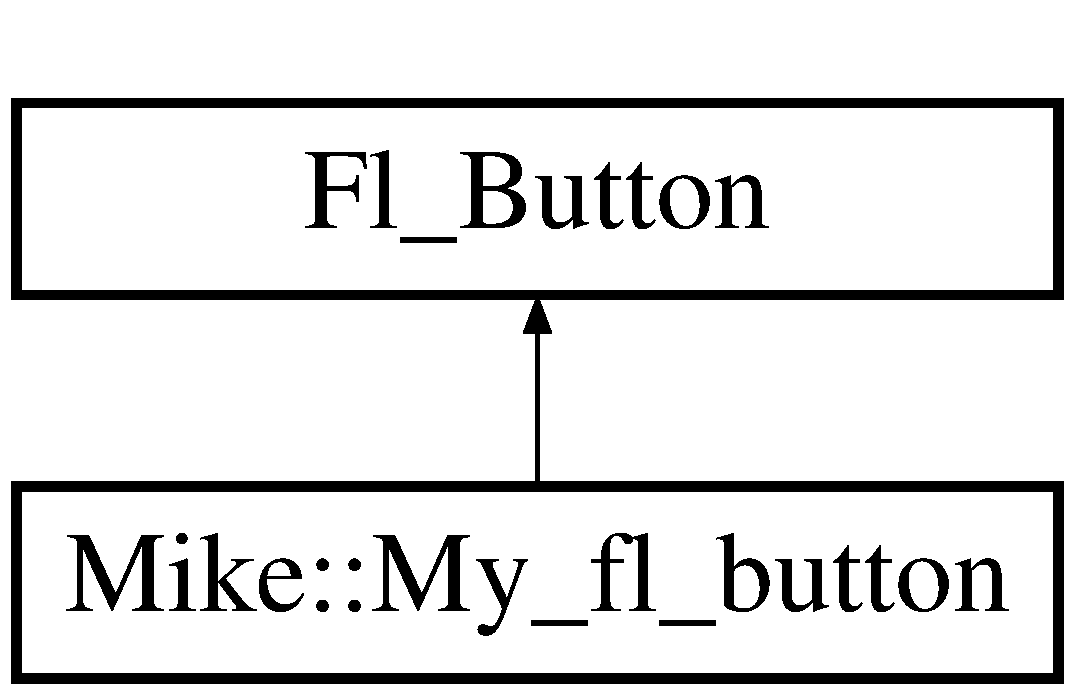
\includegraphics[height=2.000000cm]{class_mike_1_1_my__fl__button}
\end{center}
\end{figure}
\subsection*{Public Member Functions}
\begin{DoxyCompactItemize}
\item 
\hyperlink{class_mike_1_1_my__fl__button_a3339012650ecdf33d2cb219ec88e7c45}{My\+\_\+fl\+\_\+button} (int x, int y, int w, int h, const char $\ast$l)
\item 
int \hyperlink{class_mike_1_1_my__fl__button_a046314695eb006cecb6f54dc0f1057e9}{get\+Xpos} ()
\item 
int \hyperlink{class_mike_1_1_my__fl__button_a6e8291f5f02866c53ac7354b53193367}{get\+Ypos} ()
\item 
void \hyperlink{class_mike_1_1_my__fl__button_a67886921f1394ca398fb9ea3f950fa23}{set\+Ypos} (int y)
\item 
void \hyperlink{class_mike_1_1_my__fl__button_a13bb440e147816fe6ebe80d499735b60}{set\+Xpos} (int x)
\end{DoxyCompactItemize}
\subsection*{Public Attributes}
\begin{DoxyCompactItemize}
\item 
int \hyperlink{class_mike_1_1_my__fl__button_ad7b1b7c9d613dc8813fd3439b04755cf}{y\+\_\+pos}
\end{DoxyCompactItemize}
\subsection*{Protected Attributes}
\begin{DoxyCompactItemize}
\item 
int \hyperlink{class_mike_1_1_my__fl__button_aabe7efb74bd537b378072d3f1e921a72}{x\+\_\+pos}
\end{DoxyCompactItemize}


\subsection{Constructor \& Destructor Documentation}
\mbox{\Hypertarget{class_mike_1_1_my__fl__button_a3339012650ecdf33d2cb219ec88e7c45}\label{class_mike_1_1_my__fl__button_a3339012650ecdf33d2cb219ec88e7c45}} 
\index{Mike\+::\+My\+\_\+fl\+\_\+button@{Mike\+::\+My\+\_\+fl\+\_\+button}!My\+\_\+fl\+\_\+button@{My\+\_\+fl\+\_\+button}}
\index{My\+\_\+fl\+\_\+button@{My\+\_\+fl\+\_\+button}!Mike\+::\+My\+\_\+fl\+\_\+button@{Mike\+::\+My\+\_\+fl\+\_\+button}}
\subsubsection{\texorpdfstring{My\+\_\+fl\+\_\+button()}{My\_fl\_button()}}
{\footnotesize\ttfamily Mike\+::\+My\+\_\+fl\+\_\+button\+::\+My\+\_\+fl\+\_\+button (\begin{DoxyParamCaption}\item[{int}]{x,  }\item[{int}]{y,  }\item[{int}]{w,  }\item[{int}]{h,  }\item[{const char $\ast$}]{l = {\ttfamily 0} }\end{DoxyParamCaption})}



\subsection{Member Function Documentation}
\mbox{\Hypertarget{class_mike_1_1_my__fl__button_a046314695eb006cecb6f54dc0f1057e9}\label{class_mike_1_1_my__fl__button_a046314695eb006cecb6f54dc0f1057e9}} 
\index{Mike\+::\+My\+\_\+fl\+\_\+button@{Mike\+::\+My\+\_\+fl\+\_\+button}!get\+Xpos@{get\+Xpos}}
\index{get\+Xpos@{get\+Xpos}!Mike\+::\+My\+\_\+fl\+\_\+button@{Mike\+::\+My\+\_\+fl\+\_\+button}}
\subsubsection{\texorpdfstring{get\+Xpos()}{getXpos()}}
{\footnotesize\ttfamily int Mike\+::\+My\+\_\+fl\+\_\+button\+::get\+Xpos (\begin{DoxyParamCaption}{ }\end{DoxyParamCaption})\hspace{0.3cm}{\ttfamily [inline]}}

\mbox{\Hypertarget{class_mike_1_1_my__fl__button_a6e8291f5f02866c53ac7354b53193367}\label{class_mike_1_1_my__fl__button_a6e8291f5f02866c53ac7354b53193367}} 
\index{Mike\+::\+My\+\_\+fl\+\_\+button@{Mike\+::\+My\+\_\+fl\+\_\+button}!get\+Ypos@{get\+Ypos}}
\index{get\+Ypos@{get\+Ypos}!Mike\+::\+My\+\_\+fl\+\_\+button@{Mike\+::\+My\+\_\+fl\+\_\+button}}
\subsubsection{\texorpdfstring{get\+Ypos()}{getYpos()}}
{\footnotesize\ttfamily int Mike\+::\+My\+\_\+fl\+\_\+button\+::get\+Ypos (\begin{DoxyParamCaption}{ }\end{DoxyParamCaption})\hspace{0.3cm}{\ttfamily [inline]}}

\mbox{\Hypertarget{class_mike_1_1_my__fl__button_a13bb440e147816fe6ebe80d499735b60}\label{class_mike_1_1_my__fl__button_a13bb440e147816fe6ebe80d499735b60}} 
\index{Mike\+::\+My\+\_\+fl\+\_\+button@{Mike\+::\+My\+\_\+fl\+\_\+button}!set\+Xpos@{set\+Xpos}}
\index{set\+Xpos@{set\+Xpos}!Mike\+::\+My\+\_\+fl\+\_\+button@{Mike\+::\+My\+\_\+fl\+\_\+button}}
\subsubsection{\texorpdfstring{set\+Xpos()}{setXpos()}}
{\footnotesize\ttfamily void Mike\+::\+My\+\_\+fl\+\_\+button\+::set\+Xpos (\begin{DoxyParamCaption}\item[{int}]{x }\end{DoxyParamCaption})\hspace{0.3cm}{\ttfamily [inline]}}

\mbox{\Hypertarget{class_mike_1_1_my__fl__button_a67886921f1394ca398fb9ea3f950fa23}\label{class_mike_1_1_my__fl__button_a67886921f1394ca398fb9ea3f950fa23}} 
\index{Mike\+::\+My\+\_\+fl\+\_\+button@{Mike\+::\+My\+\_\+fl\+\_\+button}!set\+Ypos@{set\+Ypos}}
\index{set\+Ypos@{set\+Ypos}!Mike\+::\+My\+\_\+fl\+\_\+button@{Mike\+::\+My\+\_\+fl\+\_\+button}}
\subsubsection{\texorpdfstring{set\+Ypos()}{setYpos()}}
{\footnotesize\ttfamily void Mike\+::\+My\+\_\+fl\+\_\+button\+::set\+Ypos (\begin{DoxyParamCaption}\item[{int}]{y }\end{DoxyParamCaption})\hspace{0.3cm}{\ttfamily [inline]}}



\subsection{Member Data Documentation}
\mbox{\Hypertarget{class_mike_1_1_my__fl__button_aabe7efb74bd537b378072d3f1e921a72}\label{class_mike_1_1_my__fl__button_aabe7efb74bd537b378072d3f1e921a72}} 
\index{Mike\+::\+My\+\_\+fl\+\_\+button@{Mike\+::\+My\+\_\+fl\+\_\+button}!x\+\_\+pos@{x\+\_\+pos}}
\index{x\+\_\+pos@{x\+\_\+pos}!Mike\+::\+My\+\_\+fl\+\_\+button@{Mike\+::\+My\+\_\+fl\+\_\+button}}
\subsubsection{\texorpdfstring{x\+\_\+pos}{x\_pos}}
{\footnotesize\ttfamily int Mike\+::\+My\+\_\+fl\+\_\+button\+::x\+\_\+pos\hspace{0.3cm}{\ttfamily [protected]}}

\mbox{\Hypertarget{class_mike_1_1_my__fl__button_ad7b1b7c9d613dc8813fd3439b04755cf}\label{class_mike_1_1_my__fl__button_ad7b1b7c9d613dc8813fd3439b04755cf}} 
\index{Mike\+::\+My\+\_\+fl\+\_\+button@{Mike\+::\+My\+\_\+fl\+\_\+button}!y\+\_\+pos@{y\+\_\+pos}}
\index{y\+\_\+pos@{y\+\_\+pos}!Mike\+::\+My\+\_\+fl\+\_\+button@{Mike\+::\+My\+\_\+fl\+\_\+button}}
\subsubsection{\texorpdfstring{y\+\_\+pos}{y\_pos}}
{\footnotesize\ttfamily int Mike\+::\+My\+\_\+fl\+\_\+button\+::y\+\_\+pos}



The documentation for this class was generated from the following files\+:\begin{DoxyCompactItemize}
\item 
src/work\+In\+Progress/\hyperlink{_wid_table_base_8h}{Wid\+Table\+Base.\+h}\item 
src/work\+In\+Progress/\hyperlink{_wid_table_base_8cpp}{Wid\+Table\+Base.\+cpp}\end{DoxyCompactItemize}

\hypertarget{class_mike_1_1_user_interface}{}\section{Mike\+:\+:User\+Interface Class Reference}
\label{class_mike_1_1_user_interface}\index{Mike\+::\+User\+Interface@{Mike\+::\+User\+Interface}}


{\ttfamily \#include $<$User\+Interface.\+h$>$}

Inheritance diagram for Mike\+:\+:User\+Interface\+:\begin{figure}[H]
\begin{center}
\leavevmode
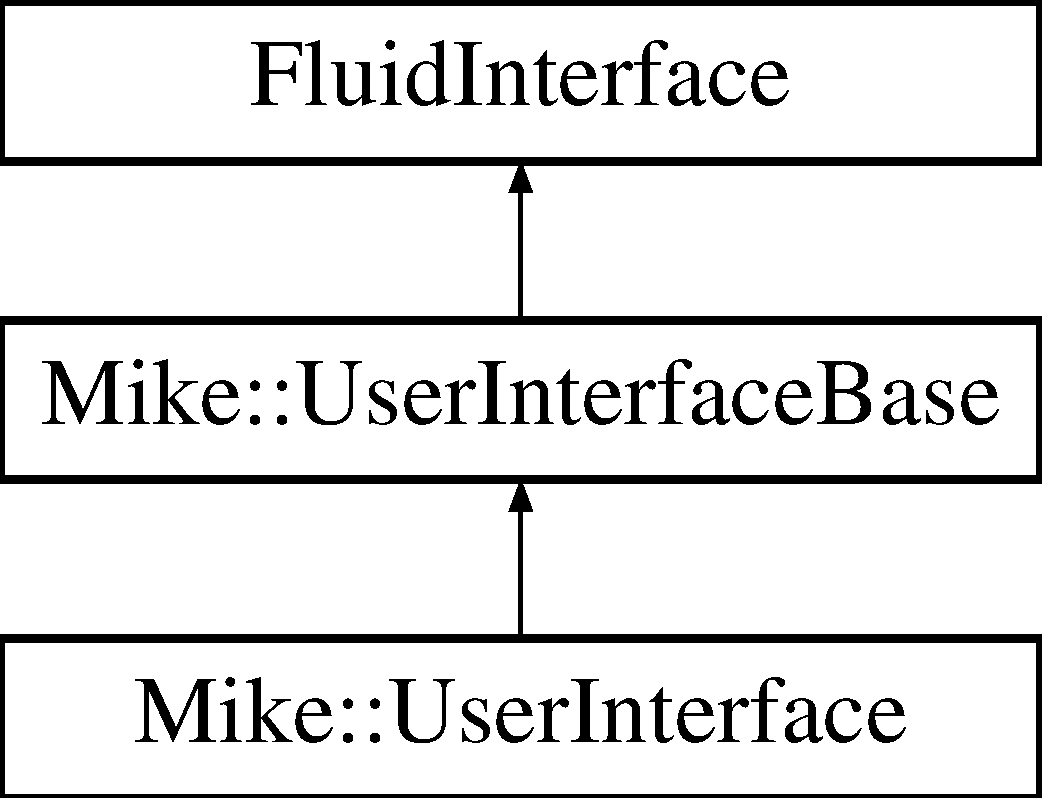
\includegraphics[height=3.000000cm]{class_mike_1_1_user_interface}
\end{center}
\end{figure}
\subsection*{Public Member Functions}
\begin{DoxyCompactItemize}
\item 
\hyperlink{class_mike_1_1_user_interface_a3c10edd966f5470fb76a7ee844de2628}{User\+Interface} (\hyperlink{class_mike_1_1_control}{Control} $\ast$control, double starting\+\_\+bid\+\_\+price=700, int number\+Of\+Columns=19, int number\+Of\+Buttoncolumns=5)
\end{DoxyCompactItemize}
\subsection*{Protected Member Functions}
\begin{DoxyCompactItemize}
\item 
virtual void \hyperlink{class_mike_1_1_user_interface_a2001cad2040c95ddea43b7d43f9e82bb}{send\+Wid\+Table\+Callback} (int row\+Pressed, int col\+Pressed, long price, \hyperlink{namespace_mike_aa486aea8b1d0d07190982a311394e6cb}{Mike\+Order\+Type} temp\+Order\+Type, int order\+Size)
\item 
virtual void \hyperlink{class_mike_1_1_user_interface_a9421dadab2852eb9110e25e2dff1d849}{callbk\+User\+Interface} (\hyperlink{namespace_mike_a9dd611fa3c671b02e477e6b21465cc66}{Btn\+Pressed})
\end{DoxyCompactItemize}
\subsection*{Additional Inherited Members}


\subsection{Constructor \& Destructor Documentation}
\mbox{\Hypertarget{class_mike_1_1_user_interface_a3c10edd966f5470fb76a7ee844de2628}\label{class_mike_1_1_user_interface_a3c10edd966f5470fb76a7ee844de2628}} 
\index{Mike\+::\+User\+Interface@{Mike\+::\+User\+Interface}!User\+Interface@{User\+Interface}}
\index{User\+Interface@{User\+Interface}!Mike\+::\+User\+Interface@{Mike\+::\+User\+Interface}}
\subsubsection{\texorpdfstring{User\+Interface()}{UserInterface()}}
{\footnotesize\ttfamily Mike\+::\+User\+Interface\+::\+User\+Interface (\begin{DoxyParamCaption}\item[{\hyperlink{class_mike_1_1_control}{Control} $\ast$}]{control,  }\item[{double}]{starting\+\_\+bid\+\_\+price = {\ttfamily 700},  }\item[{int}]{number\+Of\+Columns = {\ttfamily 19},  }\item[{int}]{number\+Of\+Buttoncolumns = {\ttfamily 5} }\end{DoxyParamCaption})}



\subsection{Member Function Documentation}
\mbox{\Hypertarget{class_mike_1_1_user_interface_a9421dadab2852eb9110e25e2dff1d849}\label{class_mike_1_1_user_interface_a9421dadab2852eb9110e25e2dff1d849}} 
\index{Mike\+::\+User\+Interface@{Mike\+::\+User\+Interface}!callbk\+User\+Interface@{callbk\+User\+Interface}}
\index{callbk\+User\+Interface@{callbk\+User\+Interface}!Mike\+::\+User\+Interface@{Mike\+::\+User\+Interface}}
\subsubsection{\texorpdfstring{callbk\+User\+Interface()}{callbkUserInterface()}}
{\footnotesize\ttfamily void Mike\+::\+User\+Interface\+::callbk\+User\+Interface (\begin{DoxyParamCaption}\item[{\hyperlink{namespace_mike_a9dd611fa3c671b02e477e6b21465cc66}{Btn\+Pressed}}]{button }\end{DoxyParamCaption})\hspace{0.3cm}{\ttfamily [protected]}, {\ttfamily [virtual]}}



Implements \hyperlink{class_mike_1_1_user_interface_base_acb35df6eb1e854e714c42f6ae473a193}{Mike\+::\+User\+Interface\+Base}.

\mbox{\Hypertarget{class_mike_1_1_user_interface_a2001cad2040c95ddea43b7d43f9e82bb}\label{class_mike_1_1_user_interface_a2001cad2040c95ddea43b7d43f9e82bb}} 
\index{Mike\+::\+User\+Interface@{Mike\+::\+User\+Interface}!send\+Wid\+Table\+Callback@{send\+Wid\+Table\+Callback}}
\index{send\+Wid\+Table\+Callback@{send\+Wid\+Table\+Callback}!Mike\+::\+User\+Interface@{Mike\+::\+User\+Interface}}
\subsubsection{\texorpdfstring{send\+Wid\+Table\+Callback()}{sendWidTableCallback()}}
{\footnotesize\ttfamily void Mike\+::\+User\+Interface\+::send\+Wid\+Table\+Callback (\begin{DoxyParamCaption}\item[{int}]{row\+Pressed,  }\item[{int}]{col\+Pressed,  }\item[{long}]{price,  }\item[{\hyperlink{namespace_mike_aa486aea8b1d0d07190982a311394e6cb}{Mike\+Order\+Type}}]{temp\+Order\+Type,  }\item[{int}]{order\+Size }\end{DoxyParamCaption})\hspace{0.3cm}{\ttfamily [protected]}, {\ttfamily [virtual]}}



Implements \hyperlink{class_mike_1_1_user_interface_base_a42469ffe57a8528064068a84e277ee6a}{Mike\+::\+User\+Interface\+Base}.



The documentation for this class was generated from the following files\+:\begin{DoxyCompactItemize}
\item 
src/work\+In\+Progress/\hyperlink{_user_interface_8h}{User\+Interface.\+h}\item 
src/work\+In\+Progress/\hyperlink{_user_interface_8cpp}{User\+Interface.\+cpp}\end{DoxyCompactItemize}

\hypertarget{class_mike_1_1_user_interface_base}{}\section{Mike\+:\+:User\+Interface\+Base Class Reference}
\label{class_mike_1_1_user_interface_base}\index{Mike\+::\+User\+Interface\+Base@{Mike\+::\+User\+Interface\+Base}}


{\ttfamily \#include $<$User\+Interface.\+h$>$}

Inheritance diagram for Mike\+:\+:User\+Interface\+Base\+:\begin{figure}[H]
\begin{center}
\leavevmode
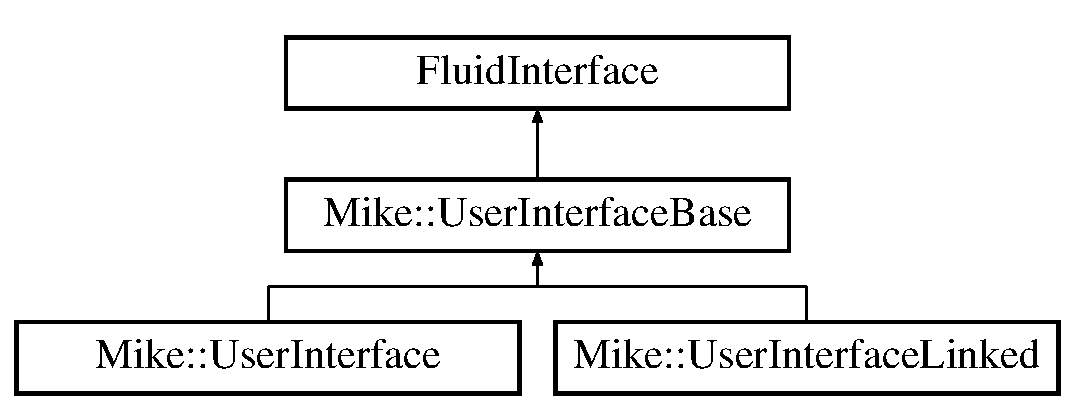
\includegraphics[height=3.000000cm]{class_mike_1_1_user_interface_base}
\end{center}
\end{figure}
\subsection*{Public Member Functions}
\begin{DoxyCompactItemize}
\item 
void \hyperlink{class_mike_1_1_user_interface_base_a8db9431a5f9fc2683908c5d4cf086623}{changename} (\+::std\+::string name)
\item 
virtual void \hyperlink{class_mike_1_1_user_interface_base_a3a1d4bc6ce2f817327d39e48340ae23c}{Print\+Bid\+Ask} (long bid, long ask)
\item 
virtual void \hyperlink{class_mike_1_1_user_interface_base_a1386d2a22c47d96264ed2549da036de3}{Print\+All} (long total\+Open\+Pos, long total\+Open\+PL, long total\+Closed\+PL, long total\+PL, long ask\+Price, long bid\+Price, const \+::std\+::vector$<$ \hyperlink{class_mike_1_1_mike_position}{Mike\+Position} $>$ $\ast$open\+Positions, const \+::std\+::vector$<$ \hyperlink{class_mike_1_1_mike_orders_at_price}{Mike\+Orders\+At\+Price} $>$ $\ast$open\+Orders\+At\+Price, double average\+Price)
\item 
void \hyperlink{class_mike_1_1_user_interface_base_a5208d9aa15d5b83eac5aca6e885dd23f}{re\+Price\+Wid\+Table} (long bidprice)
\end{DoxyCompactItemize}
\subsection*{Protected Member Functions}
\begin{DoxyCompactItemize}
\item 
\hyperlink{class_mike_1_1_user_interface_base_ada6313efe882ae0535f64cf2f3aa1aa2}{User\+Interface\+Base} ()
\item 
virtual \hyperlink{class_mike_1_1_control}{Control} $\ast$ \hyperlink{class_mike_1_1_user_interface_base_ad83087afc74a281927d47a753f752525}{Get\+Control} ()
\item 
\hyperlink{class_mike_1_1_widget_table}{Widget\+Table} $\ast$ \hyperlink{class_mike_1_1_user_interface_base_a0f9e3b0b58927dfc847c07066dd748f9}{Get\+Table} ()
\item 
virtual void \hyperlink{class_mike_1_1_user_interface_base_a42469ffe57a8528064068a84e277ee6a}{send\+Wid\+Table\+Callback} (int row\+Pressed, int col\+Pressed, long price, \hyperlink{namespace_mike_aa486aea8b1d0d07190982a311394e6cb}{Mike\+Order\+Type} temp\+Order\+Type, int order\+Size)=0
\item 
virtual void \hyperlink{class_mike_1_1_user_interface_base_acb35df6eb1e854e714c42f6ae473a193}{callbk\+User\+Interface} (\hyperlink{namespace_mike_a9dd611fa3c671b02e477e6b21465cc66}{Btn\+Pressed})=0
\item 
virtual void \hyperlink{class_mike_1_1_user_interface_base_a56229f8ce8bb05e4b9908fcfc7222412}{callbk\+Wid\+Table} (int row\+Pressed, int col\+Pressed, long price)
\item 
virtual void \hyperlink{class_mike_1_1_user_interface_base_afa6ddc0cce6cf6df28a542bd7e8c3686}{Set\+Col\+But\+Names} (\+::std\+::vector$<$\+::std\+::string $>$ \&\hyperlink{class_mike_1_1_user_interface_base_a9de8526205e04a7d4c2ea9e1486050a8}{col\+\_\+names}, \+::std\+::vector$<$\+::std\+::string $>$ \&\hyperlink{class_mike_1_1_user_interface_base_a541ac5799c899bf3dfad6532d0686bd1}{button\+\_\+names})
\end{DoxyCompactItemize}
\subsection*{Static Protected Member Functions}
\begin{DoxyCompactItemize}
\item 
static void \hyperlink{class_mike_1_1_user_interface_base_ad438c7558df623165da5070d41dd3561}{m\+\_\+reset\+Order\+Size\+\_\+cb} (Fl\+\_\+\+Widget $\ast$w, void $\ast$p)
\item 
static void \hyperlink{class_mike_1_1_user_interface_base_aeb8db80038bcb02e65b188c96a84985c}{m\+\_\+extra\+\_\+btn\+\_\+cb} (Fl\+\_\+\+Widget $\ast$w, void $\ast$p)
\item 
static void \hyperlink{class_mike_1_1_user_interface_base_a2dce036ed966a3a2ede063197ca30e1a}{m\+\_\+print\+Orders\+\_\+btn\+\_\+cb} (Fl\+\_\+\+Widget $\ast$w, void $\ast$p)
\item 
static void \hyperlink{class_mike_1_1_user_interface_base_a1f47ae3583c78cd13f3de566f1583ae3}{m\+\_\+check\+Fills\+\_\+btn\+\_\+cb} (Fl\+\_\+\+Widget $\ast$w, void $\ast$p)
\item 
static void \hyperlink{class_mike_1_1_user_interface_base_abcfd0e8bffab60ceb9892635b8b06130}{m\+\_\+print\+Pos\+\_\+btn\+\_\+cb} (Fl\+\_\+\+Widget $\ast$w, void $\ast$p)
\item 
static void \hyperlink{class_mike_1_1_user_interface_base_a29cc254adb1d358370a4be6a3ea02d8a}{m\+\_\+btn\+\_\+\+Cancel\+All\+Orders\+\_\+cb} (Fl\+\_\+\+Widget $\ast$w, void $\ast$p)
\item 
static void \hyperlink{class_mike_1_1_user_interface_base_a423d89d55cc12eee96c6d679b88313a0}{m\+\_\+btn\+\_\+\+Clear\+Postions} (Fl\+\_\+\+Widget $\ast$w, void $\ast$p)
\end{DoxyCompactItemize}
\subsection*{Protected Attributes}
\begin{DoxyCompactItemize}
\item 
\hyperlink{class_mike_1_1_widget_table}{Widget\+Table} $\ast$ \hyperlink{class_mike_1_1_user_interface_base_a56b0885c73939b643bd43f7e08f354aa}{m\+\_\+p\+Table}
\item 
\hyperlink{class_mike_1_1_control}{Control} $\ast$ \hyperlink{class_mike_1_1_user_interface_base_a54da7e6218d2c09481b0804257bd989d}{m\+\_\+p\+Control}
\item 
Fl\+\_\+\+Button $\ast$ \hyperlink{class_mike_1_1_user_interface_base_aefa6f3786f9bed8b9ec54c1a65c90b37}{m\+\_\+my\+Extra\+Btn}
\item 
int \hyperlink{class_mike_1_1_user_interface_base_a1c3c746313e0a033040696169a9f46d8}{bid\+\_\+price} = 20400
\item 
\+::std\+::vector$<$\+::std\+::string $>$ \hyperlink{class_mike_1_1_user_interface_base_a9de8526205e04a7d4c2ea9e1486050a8}{col\+\_\+names}
\item 
\+::std\+::vector$<$\+::std\+::string $>$ \hyperlink{class_mike_1_1_user_interface_base_a541ac5799c899bf3dfad6532d0686bd1}{button\+\_\+names}
\end{DoxyCompactItemize}
\subsection*{Friends}
\begin{DoxyCompactItemize}
\item 
class \hyperlink{class_mike_1_1_user_interface_base_abcbb78a2aa9a92d43c9ea7c42cbc681e}{Widget\+Table}
\item 
class \hyperlink{class_mike_1_1_user_interface_base_aa43d07603cc032a3ea563afd34b7581c}{Mike\+::\+Control}
\end{DoxyCompactItemize}
\subsection*{Additional Inherited Members}


\subsection{Constructor \& Destructor Documentation}
\mbox{\Hypertarget{class_mike_1_1_user_interface_base_ada6313efe882ae0535f64cf2f3aa1aa2}\label{class_mike_1_1_user_interface_base_ada6313efe882ae0535f64cf2f3aa1aa2}} 
\index{Mike\+::\+User\+Interface\+Base@{Mike\+::\+User\+Interface\+Base}!User\+Interface\+Base@{User\+Interface\+Base}}
\index{User\+Interface\+Base@{User\+Interface\+Base}!Mike\+::\+User\+Interface\+Base@{Mike\+::\+User\+Interface\+Base}}
\subsubsection{\texorpdfstring{User\+Interface\+Base()}{UserInterfaceBase()}}
{\footnotesize\ttfamily Mike\+::\+User\+Interface\+Base\+::\+User\+Interface\+Base (\begin{DoxyParamCaption}{ }\end{DoxyParamCaption})\hspace{0.3cm}{\ttfamily [protected]}}



\subsection{Member Function Documentation}
\mbox{\Hypertarget{class_mike_1_1_user_interface_base_acb35df6eb1e854e714c42f6ae473a193}\label{class_mike_1_1_user_interface_base_acb35df6eb1e854e714c42f6ae473a193}} 
\index{Mike\+::\+User\+Interface\+Base@{Mike\+::\+User\+Interface\+Base}!callbk\+User\+Interface@{callbk\+User\+Interface}}
\index{callbk\+User\+Interface@{callbk\+User\+Interface}!Mike\+::\+User\+Interface\+Base@{Mike\+::\+User\+Interface\+Base}}
\subsubsection{\texorpdfstring{callbk\+User\+Interface()}{callbkUserInterface()}}
{\footnotesize\ttfamily virtual void Mike\+::\+User\+Interface\+Base\+::callbk\+User\+Interface (\begin{DoxyParamCaption}\item[{\hyperlink{namespace_mike_a9dd611fa3c671b02e477e6b21465cc66}{Btn\+Pressed}}]{ }\end{DoxyParamCaption})\hspace{0.3cm}{\ttfamily [protected]}, {\ttfamily [pure virtual]}}



Implemented in \hyperlink{class_mike_1_1_user_interface_linked_a3ad33941e45f2f171cb4db443cb46841}{Mike\+::\+User\+Interface\+Linked}, and \hyperlink{class_mike_1_1_user_interface_a9421dadab2852eb9110e25e2dff1d849}{Mike\+::\+User\+Interface}.

\mbox{\Hypertarget{class_mike_1_1_user_interface_base_a56229f8ce8bb05e4b9908fcfc7222412}\label{class_mike_1_1_user_interface_base_a56229f8ce8bb05e4b9908fcfc7222412}} 
\index{Mike\+::\+User\+Interface\+Base@{Mike\+::\+User\+Interface\+Base}!callbk\+Wid\+Table@{callbk\+Wid\+Table}}
\index{callbk\+Wid\+Table@{callbk\+Wid\+Table}!Mike\+::\+User\+Interface\+Base@{Mike\+::\+User\+Interface\+Base}}
\subsubsection{\texorpdfstring{callbk\+Wid\+Table()}{callbkWidTable()}}
{\footnotesize\ttfamily void Mike\+::\+User\+Interface\+Base\+::callbk\+Wid\+Table (\begin{DoxyParamCaption}\item[{int}]{row\+Pressed,  }\item[{int}]{col\+Pressed,  }\item[{long}]{price }\end{DoxyParamCaption})\hspace{0.3cm}{\ttfamily [protected]}, {\ttfamily [virtual]}}

\mbox{\Hypertarget{class_mike_1_1_user_interface_base_a8db9431a5f9fc2683908c5d4cf086623}\label{class_mike_1_1_user_interface_base_a8db9431a5f9fc2683908c5d4cf086623}} 
\index{Mike\+::\+User\+Interface\+Base@{Mike\+::\+User\+Interface\+Base}!changename@{changename}}
\index{changename@{changename}!Mike\+::\+User\+Interface\+Base@{Mike\+::\+User\+Interface\+Base}}
\subsubsection{\texorpdfstring{changename()}{changename()}}
{\footnotesize\ttfamily void Mike\+::\+User\+Interface\+Base\+::changename (\begin{DoxyParamCaption}\item[{\+::std\+::string}]{name }\end{DoxyParamCaption})}

\mbox{\Hypertarget{class_mike_1_1_user_interface_base_ad83087afc74a281927d47a753f752525}\label{class_mike_1_1_user_interface_base_ad83087afc74a281927d47a753f752525}} 
\index{Mike\+::\+User\+Interface\+Base@{Mike\+::\+User\+Interface\+Base}!Get\+Control@{Get\+Control}}
\index{Get\+Control@{Get\+Control}!Mike\+::\+User\+Interface\+Base@{Mike\+::\+User\+Interface\+Base}}
\subsubsection{\texorpdfstring{Get\+Control()}{GetControl()}}
{\footnotesize\ttfamily virtual \hyperlink{class_mike_1_1_control}{Control}$\ast$ Mike\+::\+User\+Interface\+Base\+::\+Get\+Control (\begin{DoxyParamCaption}{ }\end{DoxyParamCaption})\hspace{0.3cm}{\ttfamily [inline]}, {\ttfamily [protected]}, {\ttfamily [virtual]}}

\mbox{\Hypertarget{class_mike_1_1_user_interface_base_a0f9e3b0b58927dfc847c07066dd748f9}\label{class_mike_1_1_user_interface_base_a0f9e3b0b58927dfc847c07066dd748f9}} 
\index{Mike\+::\+User\+Interface\+Base@{Mike\+::\+User\+Interface\+Base}!Get\+Table@{Get\+Table}}
\index{Get\+Table@{Get\+Table}!Mike\+::\+User\+Interface\+Base@{Mike\+::\+User\+Interface\+Base}}
\subsubsection{\texorpdfstring{Get\+Table()}{GetTable()}}
{\footnotesize\ttfamily \hyperlink{class_mike_1_1_widget_table}{Widget\+Table}$\ast$ Mike\+::\+User\+Interface\+Base\+::\+Get\+Table (\begin{DoxyParamCaption}{ }\end{DoxyParamCaption})\hspace{0.3cm}{\ttfamily [inline]}, {\ttfamily [protected]}}

\mbox{\Hypertarget{class_mike_1_1_user_interface_base_a29cc254adb1d358370a4be6a3ea02d8a}\label{class_mike_1_1_user_interface_base_a29cc254adb1d358370a4be6a3ea02d8a}} 
\index{Mike\+::\+User\+Interface\+Base@{Mike\+::\+User\+Interface\+Base}!m\+\_\+btn\+\_\+\+Cancel\+All\+Orders\+\_\+cb@{m\+\_\+btn\+\_\+\+Cancel\+All\+Orders\+\_\+cb}}
\index{m\+\_\+btn\+\_\+\+Cancel\+All\+Orders\+\_\+cb@{m\+\_\+btn\+\_\+\+Cancel\+All\+Orders\+\_\+cb}!Mike\+::\+User\+Interface\+Base@{Mike\+::\+User\+Interface\+Base}}
\subsubsection{\texorpdfstring{m\+\_\+btn\+\_\+\+Cancel\+All\+Orders\+\_\+cb()}{m\_btn\_CancelAllOrders\_cb()}}
{\footnotesize\ttfamily void Mike\+::\+User\+Interface\+Base\+::m\+\_\+btn\+\_\+\+Cancel\+All\+Orders\+\_\+cb (\begin{DoxyParamCaption}\item[{Fl\+\_\+\+Widget $\ast$}]{w,  }\item[{void $\ast$}]{p }\end{DoxyParamCaption})\hspace{0.3cm}{\ttfamily [static]}, {\ttfamily [protected]}}

\mbox{\Hypertarget{class_mike_1_1_user_interface_base_a423d89d55cc12eee96c6d679b88313a0}\label{class_mike_1_1_user_interface_base_a423d89d55cc12eee96c6d679b88313a0}} 
\index{Mike\+::\+User\+Interface\+Base@{Mike\+::\+User\+Interface\+Base}!m\+\_\+btn\+\_\+\+Clear\+Postions@{m\+\_\+btn\+\_\+\+Clear\+Postions}}
\index{m\+\_\+btn\+\_\+\+Clear\+Postions@{m\+\_\+btn\+\_\+\+Clear\+Postions}!Mike\+::\+User\+Interface\+Base@{Mike\+::\+User\+Interface\+Base}}
\subsubsection{\texorpdfstring{m\+\_\+btn\+\_\+\+Clear\+Postions()}{m\_btn\_ClearPostions()}}
{\footnotesize\ttfamily void Mike\+::\+User\+Interface\+Base\+::m\+\_\+btn\+\_\+\+Clear\+Postions (\begin{DoxyParamCaption}\item[{Fl\+\_\+\+Widget $\ast$}]{w,  }\item[{void $\ast$}]{p }\end{DoxyParamCaption})\hspace{0.3cm}{\ttfamily [static]}, {\ttfamily [protected]}}

\mbox{\Hypertarget{class_mike_1_1_user_interface_base_a1f47ae3583c78cd13f3de566f1583ae3}\label{class_mike_1_1_user_interface_base_a1f47ae3583c78cd13f3de566f1583ae3}} 
\index{Mike\+::\+User\+Interface\+Base@{Mike\+::\+User\+Interface\+Base}!m\+\_\+check\+Fills\+\_\+btn\+\_\+cb@{m\+\_\+check\+Fills\+\_\+btn\+\_\+cb}}
\index{m\+\_\+check\+Fills\+\_\+btn\+\_\+cb@{m\+\_\+check\+Fills\+\_\+btn\+\_\+cb}!Mike\+::\+User\+Interface\+Base@{Mike\+::\+User\+Interface\+Base}}
\subsubsection{\texorpdfstring{m\+\_\+check\+Fills\+\_\+btn\+\_\+cb()}{m\_checkFills\_btn\_cb()}}
{\footnotesize\ttfamily void Mike\+::\+User\+Interface\+Base\+::m\+\_\+check\+Fills\+\_\+btn\+\_\+cb (\begin{DoxyParamCaption}\item[{Fl\+\_\+\+Widget $\ast$}]{w,  }\item[{void $\ast$}]{p }\end{DoxyParamCaption})\hspace{0.3cm}{\ttfamily [static]}, {\ttfamily [protected]}}

\mbox{\Hypertarget{class_mike_1_1_user_interface_base_aeb8db80038bcb02e65b188c96a84985c}\label{class_mike_1_1_user_interface_base_aeb8db80038bcb02e65b188c96a84985c}} 
\index{Mike\+::\+User\+Interface\+Base@{Mike\+::\+User\+Interface\+Base}!m\+\_\+extra\+\_\+btn\+\_\+cb@{m\+\_\+extra\+\_\+btn\+\_\+cb}}
\index{m\+\_\+extra\+\_\+btn\+\_\+cb@{m\+\_\+extra\+\_\+btn\+\_\+cb}!Mike\+::\+User\+Interface\+Base@{Mike\+::\+User\+Interface\+Base}}
\subsubsection{\texorpdfstring{m\+\_\+extra\+\_\+btn\+\_\+cb()}{m\_extra\_btn\_cb()}}
{\footnotesize\ttfamily void Mike\+::\+User\+Interface\+Base\+::m\+\_\+extra\+\_\+btn\+\_\+cb (\begin{DoxyParamCaption}\item[{Fl\+\_\+\+Widget $\ast$}]{w,  }\item[{void $\ast$}]{p }\end{DoxyParamCaption})\hspace{0.3cm}{\ttfamily [static]}, {\ttfamily [protected]}}

\mbox{\Hypertarget{class_mike_1_1_user_interface_base_a2dce036ed966a3a2ede063197ca30e1a}\label{class_mike_1_1_user_interface_base_a2dce036ed966a3a2ede063197ca30e1a}} 
\index{Mike\+::\+User\+Interface\+Base@{Mike\+::\+User\+Interface\+Base}!m\+\_\+print\+Orders\+\_\+btn\+\_\+cb@{m\+\_\+print\+Orders\+\_\+btn\+\_\+cb}}
\index{m\+\_\+print\+Orders\+\_\+btn\+\_\+cb@{m\+\_\+print\+Orders\+\_\+btn\+\_\+cb}!Mike\+::\+User\+Interface\+Base@{Mike\+::\+User\+Interface\+Base}}
\subsubsection{\texorpdfstring{m\+\_\+print\+Orders\+\_\+btn\+\_\+cb()}{m\_printOrders\_btn\_cb()}}
{\footnotesize\ttfamily void Mike\+::\+User\+Interface\+Base\+::m\+\_\+print\+Orders\+\_\+btn\+\_\+cb (\begin{DoxyParamCaption}\item[{Fl\+\_\+\+Widget $\ast$}]{w,  }\item[{void $\ast$}]{p }\end{DoxyParamCaption})\hspace{0.3cm}{\ttfamily [static]}, {\ttfamily [protected]}}

\mbox{\Hypertarget{class_mike_1_1_user_interface_base_abcfd0e8bffab60ceb9892635b8b06130}\label{class_mike_1_1_user_interface_base_abcfd0e8bffab60ceb9892635b8b06130}} 
\index{Mike\+::\+User\+Interface\+Base@{Mike\+::\+User\+Interface\+Base}!m\+\_\+print\+Pos\+\_\+btn\+\_\+cb@{m\+\_\+print\+Pos\+\_\+btn\+\_\+cb}}
\index{m\+\_\+print\+Pos\+\_\+btn\+\_\+cb@{m\+\_\+print\+Pos\+\_\+btn\+\_\+cb}!Mike\+::\+User\+Interface\+Base@{Mike\+::\+User\+Interface\+Base}}
\subsubsection{\texorpdfstring{m\+\_\+print\+Pos\+\_\+btn\+\_\+cb()}{m\_printPos\_btn\_cb()}}
{\footnotesize\ttfamily void Mike\+::\+User\+Interface\+Base\+::m\+\_\+print\+Pos\+\_\+btn\+\_\+cb (\begin{DoxyParamCaption}\item[{Fl\+\_\+\+Widget $\ast$}]{w,  }\item[{void $\ast$}]{p }\end{DoxyParamCaption})\hspace{0.3cm}{\ttfamily [static]}, {\ttfamily [protected]}}

\mbox{\Hypertarget{class_mike_1_1_user_interface_base_ad438c7558df623165da5070d41dd3561}\label{class_mike_1_1_user_interface_base_ad438c7558df623165da5070d41dd3561}} 
\index{Mike\+::\+User\+Interface\+Base@{Mike\+::\+User\+Interface\+Base}!m\+\_\+reset\+Order\+Size\+\_\+cb@{m\+\_\+reset\+Order\+Size\+\_\+cb}}
\index{m\+\_\+reset\+Order\+Size\+\_\+cb@{m\+\_\+reset\+Order\+Size\+\_\+cb}!Mike\+::\+User\+Interface\+Base@{Mike\+::\+User\+Interface\+Base}}
\subsubsection{\texorpdfstring{m\+\_\+reset\+Order\+Size\+\_\+cb()}{m\_resetOrderSize\_cb()}}
{\footnotesize\ttfamily void Mike\+::\+User\+Interface\+Base\+::m\+\_\+reset\+Order\+Size\+\_\+cb (\begin{DoxyParamCaption}\item[{Fl\+\_\+\+Widget $\ast$}]{w,  }\item[{void $\ast$}]{p }\end{DoxyParamCaption})\hspace{0.3cm}{\ttfamily [static]}, {\ttfamily [protected]}}

\mbox{\Hypertarget{class_mike_1_1_user_interface_base_a1386d2a22c47d96264ed2549da036de3}\label{class_mike_1_1_user_interface_base_a1386d2a22c47d96264ed2549da036de3}} 
\index{Mike\+::\+User\+Interface\+Base@{Mike\+::\+User\+Interface\+Base}!Print\+All@{Print\+All}}
\index{Print\+All@{Print\+All}!Mike\+::\+User\+Interface\+Base@{Mike\+::\+User\+Interface\+Base}}
\subsubsection{\texorpdfstring{Print\+All()}{PrintAll()}}
{\footnotesize\ttfamily void Mike\+::\+User\+Interface\+Base\+::\+Print\+All (\begin{DoxyParamCaption}\item[{long}]{total\+Open\+Pos,  }\item[{long}]{total\+Open\+PL,  }\item[{long}]{total\+Closed\+PL,  }\item[{long}]{total\+PL,  }\item[{long}]{ask\+Price,  }\item[{long}]{bid\+Price,  }\item[{const \+::std\+::vector$<$ \hyperlink{class_mike_1_1_mike_position}{Mike\+Position} $>$ $\ast$}]{open\+Positions,  }\item[{const \+::std\+::vector$<$ \hyperlink{class_mike_1_1_mike_orders_at_price}{Mike\+Orders\+At\+Price} $>$ $\ast$}]{open\+Orders\+At\+Price,  }\item[{double}]{average\+Price }\end{DoxyParamCaption})\hspace{0.3cm}{\ttfamily [virtual]}}

\mbox{\Hypertarget{class_mike_1_1_user_interface_base_a3a1d4bc6ce2f817327d39e48340ae23c}\label{class_mike_1_1_user_interface_base_a3a1d4bc6ce2f817327d39e48340ae23c}} 
\index{Mike\+::\+User\+Interface\+Base@{Mike\+::\+User\+Interface\+Base}!Print\+Bid\+Ask@{Print\+Bid\+Ask}}
\index{Print\+Bid\+Ask@{Print\+Bid\+Ask}!Mike\+::\+User\+Interface\+Base@{Mike\+::\+User\+Interface\+Base}}
\subsubsection{\texorpdfstring{Print\+Bid\+Ask()}{PrintBidAsk()}}
{\footnotesize\ttfamily void Mike\+::\+User\+Interface\+Base\+::\+Print\+Bid\+Ask (\begin{DoxyParamCaption}\item[{long}]{bid,  }\item[{long}]{ask }\end{DoxyParamCaption})\hspace{0.3cm}{\ttfamily [virtual]}}

\mbox{\Hypertarget{class_mike_1_1_user_interface_base_a5208d9aa15d5b83eac5aca6e885dd23f}\label{class_mike_1_1_user_interface_base_a5208d9aa15d5b83eac5aca6e885dd23f}} 
\index{Mike\+::\+User\+Interface\+Base@{Mike\+::\+User\+Interface\+Base}!re\+Price\+Wid\+Table@{re\+Price\+Wid\+Table}}
\index{re\+Price\+Wid\+Table@{re\+Price\+Wid\+Table}!Mike\+::\+User\+Interface\+Base@{Mike\+::\+User\+Interface\+Base}}
\subsubsection{\texorpdfstring{re\+Price\+Wid\+Table()}{rePriceWidTable()}}
{\footnotesize\ttfamily void Mike\+::\+User\+Interface\+Base\+::re\+Price\+Wid\+Table (\begin{DoxyParamCaption}\item[{long}]{bidprice }\end{DoxyParamCaption})}

\mbox{\Hypertarget{class_mike_1_1_user_interface_base_a42469ffe57a8528064068a84e277ee6a}\label{class_mike_1_1_user_interface_base_a42469ffe57a8528064068a84e277ee6a}} 
\index{Mike\+::\+User\+Interface\+Base@{Mike\+::\+User\+Interface\+Base}!send\+Wid\+Table\+Callback@{send\+Wid\+Table\+Callback}}
\index{send\+Wid\+Table\+Callback@{send\+Wid\+Table\+Callback}!Mike\+::\+User\+Interface\+Base@{Mike\+::\+User\+Interface\+Base}}
\subsubsection{\texorpdfstring{send\+Wid\+Table\+Callback()}{sendWidTableCallback()}}
{\footnotesize\ttfamily virtual void Mike\+::\+User\+Interface\+Base\+::send\+Wid\+Table\+Callback (\begin{DoxyParamCaption}\item[{int}]{row\+Pressed,  }\item[{int}]{col\+Pressed,  }\item[{long}]{price,  }\item[{\hyperlink{namespace_mike_aa486aea8b1d0d07190982a311394e6cb}{Mike\+Order\+Type}}]{temp\+Order\+Type,  }\item[{int}]{order\+Size }\end{DoxyParamCaption})\hspace{0.3cm}{\ttfamily [protected]}, {\ttfamily [pure virtual]}}



Implemented in \hyperlink{class_mike_1_1_user_interface_linked_a687ab0f108f97cae19ee81688a45476a}{Mike\+::\+User\+Interface\+Linked}, and \hyperlink{class_mike_1_1_user_interface_a2001cad2040c95ddea43b7d43f9e82bb}{Mike\+::\+User\+Interface}.

\mbox{\Hypertarget{class_mike_1_1_user_interface_base_afa6ddc0cce6cf6df28a542bd7e8c3686}\label{class_mike_1_1_user_interface_base_afa6ddc0cce6cf6df28a542bd7e8c3686}} 
\index{Mike\+::\+User\+Interface\+Base@{Mike\+::\+User\+Interface\+Base}!Set\+Col\+But\+Names@{Set\+Col\+But\+Names}}
\index{Set\+Col\+But\+Names@{Set\+Col\+But\+Names}!Mike\+::\+User\+Interface\+Base@{Mike\+::\+User\+Interface\+Base}}
\subsubsection{\texorpdfstring{Set\+Col\+But\+Names()}{SetColButNames()}}
{\footnotesize\ttfamily void Mike\+::\+User\+Interface\+Base\+::\+Set\+Col\+But\+Names (\begin{DoxyParamCaption}\item[{\+::std\+::vector$<$\+::std\+::string $>$ \&}]{col\+\_\+names,  }\item[{\+::std\+::vector$<$\+::std\+::string $>$ \&}]{button\+\_\+names }\end{DoxyParamCaption})\hspace{0.3cm}{\ttfamily [protected]}, {\ttfamily [virtual]}}



\subsection{Friends And Related Function Documentation}
\mbox{\Hypertarget{class_mike_1_1_user_interface_base_aa43d07603cc032a3ea563afd34b7581c}\label{class_mike_1_1_user_interface_base_aa43d07603cc032a3ea563afd34b7581c}} 
\index{Mike\+::\+User\+Interface\+Base@{Mike\+::\+User\+Interface\+Base}!Mike\+::\+Control@{Mike\+::\+Control}}
\index{Mike\+::\+Control@{Mike\+::\+Control}!Mike\+::\+User\+Interface\+Base@{Mike\+::\+User\+Interface\+Base}}
\subsubsection{\texorpdfstring{Mike\+::\+Control}{Mike::Control}}
{\footnotesize\ttfamily friend class \hyperlink{class_mike_1_1_control}{Mike\+::\+Control}\hspace{0.3cm}{\ttfamily [friend]}}

\mbox{\Hypertarget{class_mike_1_1_user_interface_base_abcbb78a2aa9a92d43c9ea7c42cbc681e}\label{class_mike_1_1_user_interface_base_abcbb78a2aa9a92d43c9ea7c42cbc681e}} 
\index{Mike\+::\+User\+Interface\+Base@{Mike\+::\+User\+Interface\+Base}!Widget\+Table@{Widget\+Table}}
\index{Widget\+Table@{Widget\+Table}!Mike\+::\+User\+Interface\+Base@{Mike\+::\+User\+Interface\+Base}}
\subsubsection{\texorpdfstring{Widget\+Table}{WidgetTable}}
{\footnotesize\ttfamily friend class \hyperlink{class_mike_1_1_widget_table}{Widget\+Table}\hspace{0.3cm}{\ttfamily [friend]}}



\subsection{Member Data Documentation}
\mbox{\Hypertarget{class_mike_1_1_user_interface_base_a1c3c746313e0a033040696169a9f46d8}\label{class_mike_1_1_user_interface_base_a1c3c746313e0a033040696169a9f46d8}} 
\index{Mike\+::\+User\+Interface\+Base@{Mike\+::\+User\+Interface\+Base}!bid\+\_\+price@{bid\+\_\+price}}
\index{bid\+\_\+price@{bid\+\_\+price}!Mike\+::\+User\+Interface\+Base@{Mike\+::\+User\+Interface\+Base}}
\subsubsection{\texorpdfstring{bid\+\_\+price}{bid\_price}}
{\footnotesize\ttfamily int Mike\+::\+User\+Interface\+Base\+::bid\+\_\+price = 20400\hspace{0.3cm}{\ttfamily [protected]}}

\mbox{\Hypertarget{class_mike_1_1_user_interface_base_a541ac5799c899bf3dfad6532d0686bd1}\label{class_mike_1_1_user_interface_base_a541ac5799c899bf3dfad6532d0686bd1}} 
\index{Mike\+::\+User\+Interface\+Base@{Mike\+::\+User\+Interface\+Base}!button\+\_\+names@{button\+\_\+names}}
\index{button\+\_\+names@{button\+\_\+names}!Mike\+::\+User\+Interface\+Base@{Mike\+::\+User\+Interface\+Base}}
\subsubsection{\texorpdfstring{button\+\_\+names}{button\_names}}
{\footnotesize\ttfamily \+::std\+::vector$<$\+::std\+::string$>$ Mike\+::\+User\+Interface\+Base\+::button\+\_\+names\hspace{0.3cm}{\ttfamily [protected]}}

\mbox{\Hypertarget{class_mike_1_1_user_interface_base_a9de8526205e04a7d4c2ea9e1486050a8}\label{class_mike_1_1_user_interface_base_a9de8526205e04a7d4c2ea9e1486050a8}} 
\index{Mike\+::\+User\+Interface\+Base@{Mike\+::\+User\+Interface\+Base}!col\+\_\+names@{col\+\_\+names}}
\index{col\+\_\+names@{col\+\_\+names}!Mike\+::\+User\+Interface\+Base@{Mike\+::\+User\+Interface\+Base}}
\subsubsection{\texorpdfstring{col\+\_\+names}{col\_names}}
{\footnotesize\ttfamily \+::std\+::vector$<$\+::std\+::string$>$ Mike\+::\+User\+Interface\+Base\+::col\+\_\+names\hspace{0.3cm}{\ttfamily [protected]}}

\mbox{\Hypertarget{class_mike_1_1_user_interface_base_aefa6f3786f9bed8b9ec54c1a65c90b37}\label{class_mike_1_1_user_interface_base_aefa6f3786f9bed8b9ec54c1a65c90b37}} 
\index{Mike\+::\+User\+Interface\+Base@{Mike\+::\+User\+Interface\+Base}!m\+\_\+my\+Extra\+Btn@{m\+\_\+my\+Extra\+Btn}}
\index{m\+\_\+my\+Extra\+Btn@{m\+\_\+my\+Extra\+Btn}!Mike\+::\+User\+Interface\+Base@{Mike\+::\+User\+Interface\+Base}}
\subsubsection{\texorpdfstring{m\+\_\+my\+Extra\+Btn}{m\_myExtraBtn}}
{\footnotesize\ttfamily Fl\+\_\+\+Button$\ast$ Mike\+::\+User\+Interface\+Base\+::m\+\_\+my\+Extra\+Btn\hspace{0.3cm}{\ttfamily [protected]}}

\mbox{\Hypertarget{class_mike_1_1_user_interface_base_a54da7e6218d2c09481b0804257bd989d}\label{class_mike_1_1_user_interface_base_a54da7e6218d2c09481b0804257bd989d}} 
\index{Mike\+::\+User\+Interface\+Base@{Mike\+::\+User\+Interface\+Base}!m\+\_\+p\+Control@{m\+\_\+p\+Control}}
\index{m\+\_\+p\+Control@{m\+\_\+p\+Control}!Mike\+::\+User\+Interface\+Base@{Mike\+::\+User\+Interface\+Base}}
\subsubsection{\texorpdfstring{m\+\_\+p\+Control}{m\_pControl}}
{\footnotesize\ttfamily \hyperlink{class_mike_1_1_control}{Control}$\ast$ Mike\+::\+User\+Interface\+Base\+::m\+\_\+p\+Control\hspace{0.3cm}{\ttfamily [protected]}}

\mbox{\Hypertarget{class_mike_1_1_user_interface_base_a56b0885c73939b643bd43f7e08f354aa}\label{class_mike_1_1_user_interface_base_a56b0885c73939b643bd43f7e08f354aa}} 
\index{Mike\+::\+User\+Interface\+Base@{Mike\+::\+User\+Interface\+Base}!m\+\_\+p\+Table@{m\+\_\+p\+Table}}
\index{m\+\_\+p\+Table@{m\+\_\+p\+Table}!Mike\+::\+User\+Interface\+Base@{Mike\+::\+User\+Interface\+Base}}
\subsubsection{\texorpdfstring{m\+\_\+p\+Table}{m\_pTable}}
{\footnotesize\ttfamily \hyperlink{class_mike_1_1_widget_table}{Widget\+Table}$\ast$ Mike\+::\+User\+Interface\+Base\+::m\+\_\+p\+Table\hspace{0.3cm}{\ttfamily [protected]}}



The documentation for this class was generated from the following files\+:\begin{DoxyCompactItemize}
\item 
src/work\+In\+Progress/\hyperlink{_user_interface_8h}{User\+Interface.\+h}\item 
src/work\+In\+Progress/\hyperlink{_user_interface_8cpp}{User\+Interface.\+cpp}\end{DoxyCompactItemize}

\hypertarget{class_mike_1_1_user_interface_linked}{}\section{Mike\+:\+:User\+Interface\+Linked Class Reference}
\label{class_mike_1_1_user_interface_linked}\index{Mike\+::\+User\+Interface\+Linked@{Mike\+::\+User\+Interface\+Linked}}


{\ttfamily \#include $<$User\+Interface.\+h$>$}

Inheritance diagram for Mike\+:\+:User\+Interface\+Linked\+:\begin{figure}[H]
\begin{center}
\leavevmode
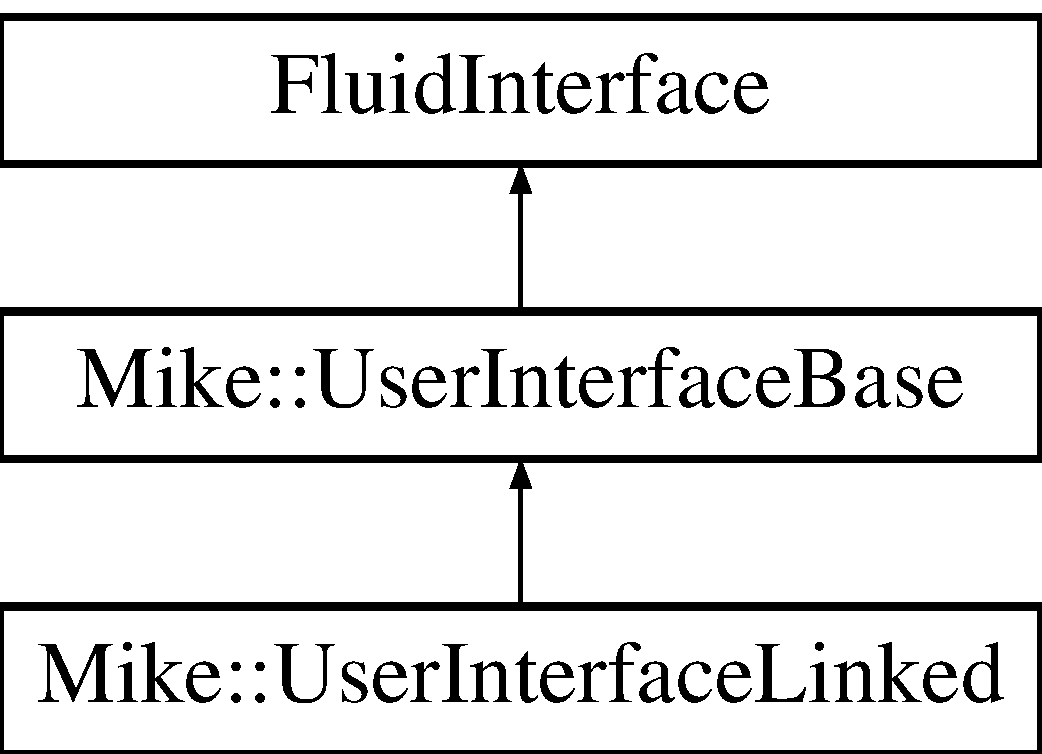
\includegraphics[height=3.000000cm]{class_mike_1_1_user_interface_linked}
\end{center}
\end{figure}
\subsection*{Public Member Functions}
\begin{DoxyCompactItemize}
\item 
\hyperlink{class_mike_1_1_user_interface_linked_aa740cbba693f1b5bb18e9415fb986a05}{User\+Interface\+Linked} (\hyperlink{class_mike_1_1_user_interface_linked_aa68f3dbce9d9f381bea2f56fda8bfb6b}{Integrator\+Pos\+UI} $\ast$ptr)
\item 
\hyperlink{class_mike_1_1_user_interface_linked_a6bae08d2fe4a3270f2bb42458d843327}{User\+Interface\+Linked} ()
\end{DoxyCompactItemize}
\subsection*{Private Member Functions}
\begin{DoxyCompactItemize}
\item 
virtual void \hyperlink{class_mike_1_1_user_interface_linked_a687ab0f108f97cae19ee81688a45476a}{send\+Wid\+Table\+Callback} (int row\+Pressed, int col\+Pressed, long price, \hyperlink{namespace_mike_aa486aea8b1d0d07190982a311394e6cb}{Mike\+Order\+Type} temp\+Order\+Type, int order\+Size)
\item 
virtual void \hyperlink{class_mike_1_1_user_interface_linked_a3ad33941e45f2f171cb4db443cb46841}{callbk\+User\+Interface} (\hyperlink{namespace_mike_a9dd611fa3c671b02e477e6b21465cc66}{Btn\+Pressed})
\end{DoxyCompactItemize}
\subsection*{Private Attributes}
\begin{DoxyCompactItemize}
\item 
\hyperlink{class_mike_1_1_user_interface_linked_aa68f3dbce9d9f381bea2f56fda8bfb6b}{Integrator\+Pos\+UI} $\ast$ \hyperlink{class_mike_1_1_user_interface_linked_aced836eb94453776afa2d07387293ea7}{callback\+Dest} = N\+U\+LL
\end{DoxyCompactItemize}
\subsection*{Friends}
\begin{DoxyCompactItemize}
\item 
class \hyperlink{class_mike_1_1_user_interface_linked_aa68f3dbce9d9f381bea2f56fda8bfb6b}{Integrator\+Pos\+UI}
\end{DoxyCompactItemize}
\subsection*{Additional Inherited Members}


\subsection{Constructor \& Destructor Documentation}
\mbox{\Hypertarget{class_mike_1_1_user_interface_linked_aa740cbba693f1b5bb18e9415fb986a05}\label{class_mike_1_1_user_interface_linked_aa740cbba693f1b5bb18e9415fb986a05}} 
\index{Mike\+::\+User\+Interface\+Linked@{Mike\+::\+User\+Interface\+Linked}!User\+Interface\+Linked@{User\+Interface\+Linked}}
\index{User\+Interface\+Linked@{User\+Interface\+Linked}!Mike\+::\+User\+Interface\+Linked@{Mike\+::\+User\+Interface\+Linked}}
\subsubsection{\texorpdfstring{User\+Interface\+Linked()}{UserInterfaceLinked()}\hspace{0.1cm}{\footnotesize\ttfamily [1/2]}}
{\footnotesize\ttfamily Mike\+::\+User\+Interface\+Linked\+::\+User\+Interface\+Linked (\begin{DoxyParamCaption}\item[{\hyperlink{class_mike_1_1_user_interface_linked_aa68f3dbce9d9f381bea2f56fda8bfb6b}{Integrator\+Pos\+UI} $\ast$}]{ptr }\end{DoxyParamCaption})}

\mbox{\Hypertarget{class_mike_1_1_user_interface_linked_a6bae08d2fe4a3270f2bb42458d843327}\label{class_mike_1_1_user_interface_linked_a6bae08d2fe4a3270f2bb42458d843327}} 
\index{Mike\+::\+User\+Interface\+Linked@{Mike\+::\+User\+Interface\+Linked}!User\+Interface\+Linked@{User\+Interface\+Linked}}
\index{User\+Interface\+Linked@{User\+Interface\+Linked}!Mike\+::\+User\+Interface\+Linked@{Mike\+::\+User\+Interface\+Linked}}
\subsubsection{\texorpdfstring{User\+Interface\+Linked()}{UserInterfaceLinked()}\hspace{0.1cm}{\footnotesize\ttfamily [2/2]}}
{\footnotesize\ttfamily Mike\+::\+User\+Interface\+Linked\+::\+User\+Interface\+Linked (\begin{DoxyParamCaption}{ }\end{DoxyParamCaption})}



\subsection{Member Function Documentation}
\mbox{\Hypertarget{class_mike_1_1_user_interface_linked_a3ad33941e45f2f171cb4db443cb46841}\label{class_mike_1_1_user_interface_linked_a3ad33941e45f2f171cb4db443cb46841}} 
\index{Mike\+::\+User\+Interface\+Linked@{Mike\+::\+User\+Interface\+Linked}!callbk\+User\+Interface@{callbk\+User\+Interface}}
\index{callbk\+User\+Interface@{callbk\+User\+Interface}!Mike\+::\+User\+Interface\+Linked@{Mike\+::\+User\+Interface\+Linked}}
\subsubsection{\texorpdfstring{callbk\+User\+Interface()}{callbkUserInterface()}}
{\footnotesize\ttfamily virtual void Mike\+::\+User\+Interface\+Linked\+::callbk\+User\+Interface (\begin{DoxyParamCaption}\item[{\hyperlink{namespace_mike_a9dd611fa3c671b02e477e6b21465cc66}{Btn\+Pressed}}]{ }\end{DoxyParamCaption})\hspace{0.3cm}{\ttfamily [private]}, {\ttfamily [virtual]}}



Implements \hyperlink{class_mike_1_1_user_interface_base_acb35df6eb1e854e714c42f6ae473a193}{Mike\+::\+User\+Interface\+Base}.

\mbox{\Hypertarget{class_mike_1_1_user_interface_linked_a687ab0f108f97cae19ee81688a45476a}\label{class_mike_1_1_user_interface_linked_a687ab0f108f97cae19ee81688a45476a}} 
\index{Mike\+::\+User\+Interface\+Linked@{Mike\+::\+User\+Interface\+Linked}!send\+Wid\+Table\+Callback@{send\+Wid\+Table\+Callback}}
\index{send\+Wid\+Table\+Callback@{send\+Wid\+Table\+Callback}!Mike\+::\+User\+Interface\+Linked@{Mike\+::\+User\+Interface\+Linked}}
\subsubsection{\texorpdfstring{send\+Wid\+Table\+Callback()}{sendWidTableCallback()}}
{\footnotesize\ttfamily virtual void Mike\+::\+User\+Interface\+Linked\+::send\+Wid\+Table\+Callback (\begin{DoxyParamCaption}\item[{int}]{row\+Pressed,  }\item[{int}]{col\+Pressed,  }\item[{long}]{price,  }\item[{\hyperlink{namespace_mike_aa486aea8b1d0d07190982a311394e6cb}{Mike\+Order\+Type}}]{temp\+Order\+Type,  }\item[{int}]{order\+Size }\end{DoxyParamCaption})\hspace{0.3cm}{\ttfamily [private]}, {\ttfamily [virtual]}}



Implements \hyperlink{class_mike_1_1_user_interface_base_a42469ffe57a8528064068a84e277ee6a}{Mike\+::\+User\+Interface\+Base}.



\subsection{Friends And Related Function Documentation}
\mbox{\Hypertarget{class_mike_1_1_user_interface_linked_aa68f3dbce9d9f381bea2f56fda8bfb6b}\label{class_mike_1_1_user_interface_linked_aa68f3dbce9d9f381bea2f56fda8bfb6b}} 
\index{Mike\+::\+User\+Interface\+Linked@{Mike\+::\+User\+Interface\+Linked}!Integrator\+Pos\+UI@{Integrator\+Pos\+UI}}
\index{Integrator\+Pos\+UI@{Integrator\+Pos\+UI}!Mike\+::\+User\+Interface\+Linked@{Mike\+::\+User\+Interface\+Linked}}
\subsubsection{\texorpdfstring{Integrator\+Pos\+UI}{IntegratorPosUI}}
{\footnotesize\ttfamily friend class Integrator\+Pos\+UI\hspace{0.3cm}{\ttfamily [friend]}}



\subsection{Member Data Documentation}
\mbox{\Hypertarget{class_mike_1_1_user_interface_linked_aced836eb94453776afa2d07387293ea7}\label{class_mike_1_1_user_interface_linked_aced836eb94453776afa2d07387293ea7}} 
\index{Mike\+::\+User\+Interface\+Linked@{Mike\+::\+User\+Interface\+Linked}!callback\+Dest@{callback\+Dest}}
\index{callback\+Dest@{callback\+Dest}!Mike\+::\+User\+Interface\+Linked@{Mike\+::\+User\+Interface\+Linked}}
\subsubsection{\texorpdfstring{callback\+Dest}{callbackDest}}
{\footnotesize\ttfamily \hyperlink{class_mike_1_1_user_interface_linked_aa68f3dbce9d9f381bea2f56fda8bfb6b}{Integrator\+Pos\+UI}$\ast$ Mike\+::\+User\+Interface\+Linked\+::callback\+Dest = N\+U\+LL\hspace{0.3cm}{\ttfamily [private]}}



The documentation for this class was generated from the following file\+:\begin{DoxyCompactItemize}
\item 
src/work\+In\+Progress/\hyperlink{_user_interface_8h}{User\+Interface.\+h}\end{DoxyCompactItemize}

\hypertarget{class_mike_1_1_widget_table}{}\section{Mike\+:\+:Widget\+Table Class Reference}
\label{class_mike_1_1_widget_table}\index{Mike\+::\+Widget\+Table@{Mike\+::\+Widget\+Table}}


{\ttfamily \#include $<$Widget\+Table.\+h$>$}

Inheritance diagram for Mike\+:\+:Widget\+Table\+:\begin{figure}[H]
\begin{center}
\leavevmode
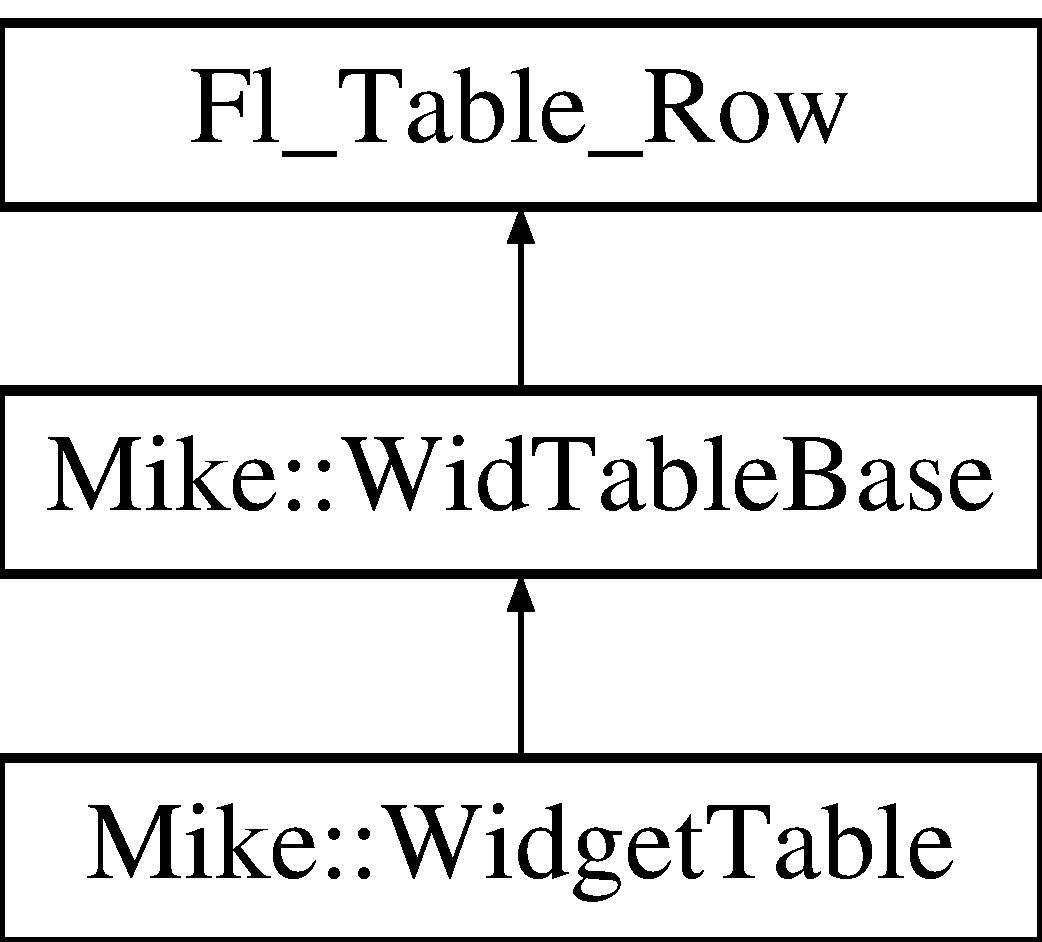
\includegraphics[height=3.000000cm]{class_mike_1_1_widget_table}
\end{center}
\end{figure}
\subsection*{Public Member Functions}
\begin{DoxyCompactItemize}
\item 
\hyperlink{class_mike_1_1_widget_table_a2b409a5c6b7f2f4fd589ac0250fc297d}{Widget\+Table} (int x, int y, int w, int h, const char $\ast$l, \hyperlink{class_mike_1_1_user_interface_base}{User\+Interface\+Base} $\ast$p\+User\+Interface, int top\+\_\+row\+\_\+price, int number\+\_\+rows, int number\+\_\+cols, int how\+\_\+many\+\_\+cols\+\_\+are\+\_\+buttons=5, std\+::vector$<$ std\+::string $>$ \hyperlink{class_mike_1_1_wid_table_base_acc76591b1fa97f8259fc95f492d8e1b9}{col\+\_\+names}=\{ \char`\"{}\char`\"{} \}, std\+::vector$<$ std\+::string $>$ button\+\_\+names=\{ \char`\"{}\char`\"{} \})
\item 
\hyperlink{class_mike_1_1_widget_table_a1989e5265f9e1d53512d5936d21d41b5}{Widget\+Table} (int x, int y, int w, int h, const char $\ast$l)
\item 
\hyperlink{class_mike_1_1_widget_table_a141dd523d530477be58523c3ae2c2365}{Widget\+Table} ()
\item 
virtual void \hyperlink{class_mike_1_1_widget_table_a4a798ce9e43334f3ee1823c89ee91cf3}{print\+Bid\+Ask} (long bid, long ask)
\item 
virtual void \hyperlink{class_mike_1_1_widget_table_a8e269ede4b6a6ca1ef70ef588aa5e601}{print\+Positions} (const std\+::vector$<$ \hyperlink{class_mike_1_1_mike_position}{Mike\+Position} $>$ $\ast$open\+Positions)
\item 
virtual void \hyperlink{class_mike_1_1_widget_table_a4ed53614a2ef8bc68994a84af4b30084}{print\+Positions} (const std\+::vector$<$ \hyperlink{class_mike_1_1_mike_position}{Mike\+Position} $>$ $\ast$open\+Positions, const std\+::vector$<$ \hyperlink{class_mike_1_1_mike_orders_at_price}{Mike\+Orders\+At\+Price} $>$ $\ast$open\+Orders\+At\+Price)
\item 
virtual short \hyperlink{class_mike_1_1_widget_table_a72cefeed8a17eb9abea21c3f38d7fe23}{Get\+Bid\+Col} ()
\item 
virtual short \hyperlink{class_mike_1_1_widget_table_a7f23d041f5d4eab8103cca41951f7863}{Get\+Ask\+Col} ()
\end{DoxyCompactItemize}
\subsection*{Public Attributes}
\begin{DoxyCompactItemize}
\item 
bool \hyperlink{class_mike_1_1_widget_table_a4036058693902d510469a59b9466a366}{widget\+Table\+Needs\+Clear\+All} = true
\end{DoxyCompactItemize}
\subsection*{Protected Member Functions}
\begin{DoxyCompactItemize}
\item 
virtual void \hyperlink{class_mike_1_1_widget_table_affddec39940626f7d72ffaf9e02d04e4}{virt\+Button\+Cb} (Fl\+\_\+\+Widget $\ast$w, void $\ast$p)
\item 
virtual void \hyperlink{class_mike_1_1_widget_table_ae788064f6ed7b19e9ac42b717ff53567}{set\+Bid\+Ask\+Columns} ()
\item 
\hyperlink{class_mike_1_1_user_interface_base}{User\+Interface\+Base} $\ast$ \hyperlink{class_mike_1_1_widget_table_a62d2aadd2ee9f9e9f376dd597b5dcd7b}{Get\+User\+Interface} ()
\item 
\hyperlink{class_mike_1_1_control}{Control} $\ast$ \hyperlink{class_mike_1_1_widget_table_ad5fd734ccfa48b6866554122c8b66667}{Get\+Control} ()
\item 
void \hyperlink{class_mike_1_1_widget_table_a7c161d452ff10617cafcbc331a92a8b2}{Pop\+Price\+Col} ()
\end{DoxyCompactItemize}
\subsection*{Protected Attributes}
\begin{DoxyCompactItemize}
\item 
\hyperlink{class_mike_1_1_user_interface_base}{User\+Interface\+Base} $\ast$ \hyperlink{class_mike_1_1_widget_table_a460f10100176575e81fdab9aa342f1fc}{ptr\+\_\+to\+\_\+\+User\+Interface}
\item 
\hyperlink{class_mike_1_1_control}{Control} $\ast$ \hyperlink{class_mike_1_1_widget_table_a99eeaeb402037858e27985daf341c295}{ptr\+Control}
\item 
std\+::set$<$ long $>$ \hyperlink{class_mike_1_1_widget_table_a2be8c41838500d0e8cc343f873123627}{usedprices}
\item 
std\+::set$<$ long $>$ \hyperlink{class_mike_1_1_widget_table_a4a046800392a9e7685f8650495b938aa}{notusedprices}
\item 
short \hyperlink{class_mike_1_1_widget_table_a11872a3f7b12c24408afa775e535b355}{price\+Col} = 5
\item 
short \hyperlink{class_mike_1_1_widget_table_a4e008648f0bc010c2bbde1fc549002b7}{bid\+Column} = 6
\item 
short \hyperlink{class_mike_1_1_widget_table_aa7a40e478418cd985cade406cbd842bf}{ask\+Column} = 7
\item 
short \hyperlink{class_mike_1_1_widget_table_ac3572ce4e7d0c7aa5a1fcca70cbdb9fd}{buy\+Limit\+Order\+Col} = 8
\item 
short \hyperlink{class_mike_1_1_widget_table_a11086c367b264f5f89c81d84a57175f1}{buy\+Stop\+Order\+Col} = 9
\item 
short \hyperlink{class_mike_1_1_widget_table_a0c380b42a2fdd90e5611c178459a0220}{sell\+Limit\+Order\+Col} = 10
\item 
short \hyperlink{class_mike_1_1_widget_table_ab2ccfe721d6f46bec502537be80500b0}{sell\+Stop\+Order\+Col} = 11
\item 
short \hyperlink{class_mike_1_1_widget_table_a22fc35da5771db1fabacf89707e1460e}{open\+Pos\+Col} = 12
\item 
short \hyperlink{class_mike_1_1_widget_table_a6d455e6428a049b73ca5abc431b2e435}{open\+P\+L\+Col} = 13
\item 
short \hyperlink{class_mike_1_1_widget_table_a4f69dde53abb4ecf06a6c773f002e174}{closed\+P\+L\+Col} = 14
\item 
short \hyperlink{class_mike_1_1_widget_table_acff6706430ba0825b29cefd5f4cac752}{total\+P\+L\+Col} = 15
\item 
short \hyperlink{class_mike_1_1_widget_table_a1663756da4a083698f606af83a1b2447}{avg\+Price\+Col} = 5
\item 
short \hyperlink{class_mike_1_1_widget_table_a16ce4e53a1c455b630399f87d154e5ed}{windownumber} = 0
\end{DoxyCompactItemize}
\subsection*{Friends}
\begin{DoxyCompactItemize}
\item 
class \hyperlink{class_mike_1_1_widget_table_a530ab6298efc8f8abbe63608c9c3e996}{User\+Interface\+Base}
\item 
class \hyperlink{class_mike_1_1_widget_table_adb55a5cf0f8d4b17f324a902a7904d97}{User\+Interface}
\end{DoxyCompactItemize}
\subsection*{Additional Inherited Members}


\subsection{Constructor \& Destructor Documentation}
\mbox{\Hypertarget{class_mike_1_1_widget_table_a2b409a5c6b7f2f4fd589ac0250fc297d}\label{class_mike_1_1_widget_table_a2b409a5c6b7f2f4fd589ac0250fc297d}} 
\index{Mike\+::\+Widget\+Table@{Mike\+::\+Widget\+Table}!Widget\+Table@{Widget\+Table}}
\index{Widget\+Table@{Widget\+Table}!Mike\+::\+Widget\+Table@{Mike\+::\+Widget\+Table}}
\subsubsection{\texorpdfstring{Widget\+Table()}{WidgetTable()}\hspace{0.1cm}{\footnotesize\ttfamily [1/3]}}
{\footnotesize\ttfamily Mike\+::\+Widget\+Table\+::\+Widget\+Table (\begin{DoxyParamCaption}\item[{int}]{x,  }\item[{int}]{y,  }\item[{int}]{w,  }\item[{int}]{h,  }\item[{const char $\ast$}]{l,  }\item[{\hyperlink{class_mike_1_1_user_interface_base}{User\+Interface\+Base} $\ast$}]{p\+User\+Interface,  }\item[{int}]{top\+\_\+row\+\_\+price,  }\item[{int}]{number\+\_\+rows,  }\item[{int}]{number\+\_\+cols,  }\item[{int}]{how\+\_\+many\+\_\+cols\+\_\+are\+\_\+buttons = {\ttfamily 5},  }\item[{std\+::vector$<$ std\+::string $>$}]{col\+\_\+names = {\ttfamily \{~\char`\"{}\char`\"{}~\}},  }\item[{std\+::vector$<$ std\+::string $>$}]{button\+\_\+names = {\ttfamily \{~\char`\"{}\char`\"{}~\}} }\end{DoxyParamCaption})}

\mbox{\Hypertarget{class_mike_1_1_widget_table_a1989e5265f9e1d53512d5936d21d41b5}\label{class_mike_1_1_widget_table_a1989e5265f9e1d53512d5936d21d41b5}} 
\index{Mike\+::\+Widget\+Table@{Mike\+::\+Widget\+Table}!Widget\+Table@{Widget\+Table}}
\index{Widget\+Table@{Widget\+Table}!Mike\+::\+Widget\+Table@{Mike\+::\+Widget\+Table}}
\subsubsection{\texorpdfstring{Widget\+Table()}{WidgetTable()}\hspace{0.1cm}{\footnotesize\ttfamily [2/3]}}
{\footnotesize\ttfamily Mike\+::\+Widget\+Table\+::\+Widget\+Table (\begin{DoxyParamCaption}\item[{int}]{x,  }\item[{int}]{y,  }\item[{int}]{w,  }\item[{int}]{h,  }\item[{const char $\ast$}]{l }\end{DoxyParamCaption})}

\mbox{\Hypertarget{class_mike_1_1_widget_table_a141dd523d530477be58523c3ae2c2365}\label{class_mike_1_1_widget_table_a141dd523d530477be58523c3ae2c2365}} 
\index{Mike\+::\+Widget\+Table@{Mike\+::\+Widget\+Table}!Widget\+Table@{Widget\+Table}}
\index{Widget\+Table@{Widget\+Table}!Mike\+::\+Widget\+Table@{Mike\+::\+Widget\+Table}}
\subsubsection{\texorpdfstring{Widget\+Table()}{WidgetTable()}\hspace{0.1cm}{\footnotesize\ttfamily [3/3]}}
{\footnotesize\ttfamily Mike\+::\+Widget\+Table\+::\+Widget\+Table (\begin{DoxyParamCaption}{ }\end{DoxyParamCaption})}



\subsection{Member Function Documentation}
\mbox{\Hypertarget{class_mike_1_1_widget_table_a7f23d041f5d4eab8103cca41951f7863}\label{class_mike_1_1_widget_table_a7f23d041f5d4eab8103cca41951f7863}} 
\index{Mike\+::\+Widget\+Table@{Mike\+::\+Widget\+Table}!Get\+Ask\+Col@{Get\+Ask\+Col}}
\index{Get\+Ask\+Col@{Get\+Ask\+Col}!Mike\+::\+Widget\+Table@{Mike\+::\+Widget\+Table}}
\subsubsection{\texorpdfstring{Get\+Ask\+Col()}{GetAskCol()}}
{\footnotesize\ttfamily virtual short Mike\+::\+Widget\+Table\+::\+Get\+Ask\+Col (\begin{DoxyParamCaption}{ }\end{DoxyParamCaption})\hspace{0.3cm}{\ttfamily [inline]}, {\ttfamily [virtual]}}

\mbox{\Hypertarget{class_mike_1_1_widget_table_a72cefeed8a17eb9abea21c3f38d7fe23}\label{class_mike_1_1_widget_table_a72cefeed8a17eb9abea21c3f38d7fe23}} 
\index{Mike\+::\+Widget\+Table@{Mike\+::\+Widget\+Table}!Get\+Bid\+Col@{Get\+Bid\+Col}}
\index{Get\+Bid\+Col@{Get\+Bid\+Col}!Mike\+::\+Widget\+Table@{Mike\+::\+Widget\+Table}}
\subsubsection{\texorpdfstring{Get\+Bid\+Col()}{GetBidCol()}}
{\footnotesize\ttfamily virtual short Mike\+::\+Widget\+Table\+::\+Get\+Bid\+Col (\begin{DoxyParamCaption}{ }\end{DoxyParamCaption})\hspace{0.3cm}{\ttfamily [inline]}, {\ttfamily [virtual]}}

\mbox{\Hypertarget{class_mike_1_1_widget_table_ad5fd734ccfa48b6866554122c8b66667}\label{class_mike_1_1_widget_table_ad5fd734ccfa48b6866554122c8b66667}} 
\index{Mike\+::\+Widget\+Table@{Mike\+::\+Widget\+Table}!Get\+Control@{Get\+Control}}
\index{Get\+Control@{Get\+Control}!Mike\+::\+Widget\+Table@{Mike\+::\+Widget\+Table}}
\subsubsection{\texorpdfstring{Get\+Control()}{GetControl()}}
{\footnotesize\ttfamily \hyperlink{class_mike_1_1_control}{Control}$\ast$ Mike\+::\+Widget\+Table\+::\+Get\+Control (\begin{DoxyParamCaption}{ }\end{DoxyParamCaption})\hspace{0.3cm}{\ttfamily [inline]}, {\ttfamily [protected]}}

\mbox{\Hypertarget{class_mike_1_1_widget_table_a62d2aadd2ee9f9e9f376dd597b5dcd7b}\label{class_mike_1_1_widget_table_a62d2aadd2ee9f9e9f376dd597b5dcd7b}} 
\index{Mike\+::\+Widget\+Table@{Mike\+::\+Widget\+Table}!Get\+User\+Interface@{Get\+User\+Interface}}
\index{Get\+User\+Interface@{Get\+User\+Interface}!Mike\+::\+Widget\+Table@{Mike\+::\+Widget\+Table}}
\subsubsection{\texorpdfstring{Get\+User\+Interface()}{GetUserInterface()}}
{\footnotesize\ttfamily \hyperlink{class_mike_1_1_user_interface_base}{User\+Interface\+Base}$\ast$ Mike\+::\+Widget\+Table\+::\+Get\+User\+Interface (\begin{DoxyParamCaption}{ }\end{DoxyParamCaption})\hspace{0.3cm}{\ttfamily [inline]}, {\ttfamily [protected]}}

\mbox{\Hypertarget{class_mike_1_1_widget_table_a7c161d452ff10617cafcbc331a92a8b2}\label{class_mike_1_1_widget_table_a7c161d452ff10617cafcbc331a92a8b2}} 
\index{Mike\+::\+Widget\+Table@{Mike\+::\+Widget\+Table}!Pop\+Price\+Col@{Pop\+Price\+Col}}
\index{Pop\+Price\+Col@{Pop\+Price\+Col}!Mike\+::\+Widget\+Table@{Mike\+::\+Widget\+Table}}
\subsubsection{\texorpdfstring{Pop\+Price\+Col()}{PopPriceCol()}}
{\footnotesize\ttfamily void Mike\+::\+Widget\+Table\+::\+Pop\+Price\+Col (\begin{DoxyParamCaption}{ }\end{DoxyParamCaption})\hspace{0.3cm}{\ttfamily [protected]}}

\mbox{\Hypertarget{class_mike_1_1_widget_table_a4a798ce9e43334f3ee1823c89ee91cf3}\label{class_mike_1_1_widget_table_a4a798ce9e43334f3ee1823c89ee91cf3}} 
\index{Mike\+::\+Widget\+Table@{Mike\+::\+Widget\+Table}!print\+Bid\+Ask@{print\+Bid\+Ask}}
\index{print\+Bid\+Ask@{print\+Bid\+Ask}!Mike\+::\+Widget\+Table@{Mike\+::\+Widget\+Table}}
\subsubsection{\texorpdfstring{print\+Bid\+Ask()}{printBidAsk()}}
{\footnotesize\ttfamily virtual void Mike\+::\+Widget\+Table\+::print\+Bid\+Ask (\begin{DoxyParamCaption}\item[{long}]{bid,  }\item[{long}]{ask }\end{DoxyParamCaption})\hspace{0.3cm}{\ttfamily [inline]}, {\ttfamily [virtual]}}

\mbox{\Hypertarget{class_mike_1_1_widget_table_a8e269ede4b6a6ca1ef70ef588aa5e601}\label{class_mike_1_1_widget_table_a8e269ede4b6a6ca1ef70ef588aa5e601}} 
\index{Mike\+::\+Widget\+Table@{Mike\+::\+Widget\+Table}!print\+Positions@{print\+Positions}}
\index{print\+Positions@{print\+Positions}!Mike\+::\+Widget\+Table@{Mike\+::\+Widget\+Table}}
\subsubsection{\texorpdfstring{print\+Positions()}{printPositions()}\hspace{0.1cm}{\footnotesize\ttfamily [1/2]}}
{\footnotesize\ttfamily virtual void Mike\+::\+Widget\+Table\+::print\+Positions (\begin{DoxyParamCaption}\item[{const std\+::vector$<$ \hyperlink{class_mike_1_1_mike_position}{Mike\+Position} $>$ $\ast$}]{open\+Positions }\end{DoxyParamCaption})\hspace{0.3cm}{\ttfamily [inline]}, {\ttfamily [virtual]}}

\mbox{\Hypertarget{class_mike_1_1_widget_table_a4ed53614a2ef8bc68994a84af4b30084}\label{class_mike_1_1_widget_table_a4ed53614a2ef8bc68994a84af4b30084}} 
\index{Mike\+::\+Widget\+Table@{Mike\+::\+Widget\+Table}!print\+Positions@{print\+Positions}}
\index{print\+Positions@{print\+Positions}!Mike\+::\+Widget\+Table@{Mike\+::\+Widget\+Table}}
\subsubsection{\texorpdfstring{print\+Positions()}{printPositions()}\hspace{0.1cm}{\footnotesize\ttfamily [2/2]}}
{\footnotesize\ttfamily void Mike\+::\+Widget\+Table\+::print\+Positions (\begin{DoxyParamCaption}\item[{const std\+::vector$<$ \hyperlink{class_mike_1_1_mike_position}{Mike\+Position} $>$ $\ast$}]{open\+Positions,  }\item[{const std\+::vector$<$ \hyperlink{class_mike_1_1_mike_orders_at_price}{Mike\+Orders\+At\+Price} $>$ $\ast$}]{open\+Orders\+At\+Price }\end{DoxyParamCaption})\hspace{0.3cm}{\ttfamily [virtual]}}

\mbox{\Hypertarget{class_mike_1_1_widget_table_ae788064f6ed7b19e9ac42b717ff53567}\label{class_mike_1_1_widget_table_ae788064f6ed7b19e9ac42b717ff53567}} 
\index{Mike\+::\+Widget\+Table@{Mike\+::\+Widget\+Table}!set\+Bid\+Ask\+Columns@{set\+Bid\+Ask\+Columns}}
\index{set\+Bid\+Ask\+Columns@{set\+Bid\+Ask\+Columns}!Mike\+::\+Widget\+Table@{Mike\+::\+Widget\+Table}}
\subsubsection{\texorpdfstring{set\+Bid\+Ask\+Columns()}{setBidAskColumns()}}
{\footnotesize\ttfamily void Mike\+::\+Widget\+Table\+::set\+Bid\+Ask\+Columns (\begin{DoxyParamCaption}{ }\end{DoxyParamCaption})\hspace{0.3cm}{\ttfamily [protected]}, {\ttfamily [virtual]}}

\mbox{\Hypertarget{class_mike_1_1_widget_table_affddec39940626f7d72ffaf9e02d04e4}\label{class_mike_1_1_widget_table_affddec39940626f7d72ffaf9e02d04e4}} 
\index{Mike\+::\+Widget\+Table@{Mike\+::\+Widget\+Table}!virt\+Button\+Cb@{virt\+Button\+Cb}}
\index{virt\+Button\+Cb@{virt\+Button\+Cb}!Mike\+::\+Widget\+Table@{Mike\+::\+Widget\+Table}}
\subsubsection{\texorpdfstring{virt\+Button\+Cb()}{virtButtonCb()}}
{\footnotesize\ttfamily void Mike\+::\+Widget\+Table\+::virt\+Button\+Cb (\begin{DoxyParamCaption}\item[{Fl\+\_\+\+Widget $\ast$}]{w,  }\item[{void $\ast$}]{p }\end{DoxyParamCaption})\hspace{0.3cm}{\ttfamily [protected]}, {\ttfamily [virtual]}}



Reimplemented from \hyperlink{class_mike_1_1_wid_table_base_aed65d79c6e84fd89abceaf6ffa079fad}{Mike\+::\+Wid\+Table\+Base}.



\subsection{Friends And Related Function Documentation}
\mbox{\Hypertarget{class_mike_1_1_widget_table_adb55a5cf0f8d4b17f324a902a7904d97}\label{class_mike_1_1_widget_table_adb55a5cf0f8d4b17f324a902a7904d97}} 
\index{Mike\+::\+Widget\+Table@{Mike\+::\+Widget\+Table}!User\+Interface@{User\+Interface}}
\index{User\+Interface@{User\+Interface}!Mike\+::\+Widget\+Table@{Mike\+::\+Widget\+Table}}
\subsubsection{\texorpdfstring{User\+Interface}{UserInterface}}
{\footnotesize\ttfamily friend class \hyperlink{class_mike_1_1_user_interface}{User\+Interface}\hspace{0.3cm}{\ttfamily [friend]}}

\mbox{\Hypertarget{class_mike_1_1_widget_table_a530ab6298efc8f8abbe63608c9c3e996}\label{class_mike_1_1_widget_table_a530ab6298efc8f8abbe63608c9c3e996}} 
\index{Mike\+::\+Widget\+Table@{Mike\+::\+Widget\+Table}!User\+Interface\+Base@{User\+Interface\+Base}}
\index{User\+Interface\+Base@{User\+Interface\+Base}!Mike\+::\+Widget\+Table@{Mike\+::\+Widget\+Table}}
\subsubsection{\texorpdfstring{User\+Interface\+Base}{UserInterfaceBase}}
{\footnotesize\ttfamily friend class \hyperlink{class_mike_1_1_user_interface_base}{User\+Interface\+Base}\hspace{0.3cm}{\ttfamily [friend]}}



\subsection{Member Data Documentation}
\mbox{\Hypertarget{class_mike_1_1_widget_table_aa7a40e478418cd985cade406cbd842bf}\label{class_mike_1_1_widget_table_aa7a40e478418cd985cade406cbd842bf}} 
\index{Mike\+::\+Widget\+Table@{Mike\+::\+Widget\+Table}!ask\+Column@{ask\+Column}}
\index{ask\+Column@{ask\+Column}!Mike\+::\+Widget\+Table@{Mike\+::\+Widget\+Table}}
\subsubsection{\texorpdfstring{ask\+Column}{askColumn}}
{\footnotesize\ttfamily short Mike\+::\+Widget\+Table\+::ask\+Column = 7\hspace{0.3cm}{\ttfamily [protected]}}

\mbox{\Hypertarget{class_mike_1_1_widget_table_a1663756da4a083698f606af83a1b2447}\label{class_mike_1_1_widget_table_a1663756da4a083698f606af83a1b2447}} 
\index{Mike\+::\+Widget\+Table@{Mike\+::\+Widget\+Table}!avg\+Price\+Col@{avg\+Price\+Col}}
\index{avg\+Price\+Col@{avg\+Price\+Col}!Mike\+::\+Widget\+Table@{Mike\+::\+Widget\+Table}}
\subsubsection{\texorpdfstring{avg\+Price\+Col}{avgPriceCol}}
{\footnotesize\ttfamily short Mike\+::\+Widget\+Table\+::avg\+Price\+Col = 5\hspace{0.3cm}{\ttfamily [protected]}}

\mbox{\Hypertarget{class_mike_1_1_widget_table_a4e008648f0bc010c2bbde1fc549002b7}\label{class_mike_1_1_widget_table_a4e008648f0bc010c2bbde1fc549002b7}} 
\index{Mike\+::\+Widget\+Table@{Mike\+::\+Widget\+Table}!bid\+Column@{bid\+Column}}
\index{bid\+Column@{bid\+Column}!Mike\+::\+Widget\+Table@{Mike\+::\+Widget\+Table}}
\subsubsection{\texorpdfstring{bid\+Column}{bidColumn}}
{\footnotesize\ttfamily short Mike\+::\+Widget\+Table\+::bid\+Column = 6\hspace{0.3cm}{\ttfamily [protected]}}

\mbox{\Hypertarget{class_mike_1_1_widget_table_ac3572ce4e7d0c7aa5a1fcca70cbdb9fd}\label{class_mike_1_1_widget_table_ac3572ce4e7d0c7aa5a1fcca70cbdb9fd}} 
\index{Mike\+::\+Widget\+Table@{Mike\+::\+Widget\+Table}!buy\+Limit\+Order\+Col@{buy\+Limit\+Order\+Col}}
\index{buy\+Limit\+Order\+Col@{buy\+Limit\+Order\+Col}!Mike\+::\+Widget\+Table@{Mike\+::\+Widget\+Table}}
\subsubsection{\texorpdfstring{buy\+Limit\+Order\+Col}{buyLimitOrderCol}}
{\footnotesize\ttfamily short Mike\+::\+Widget\+Table\+::buy\+Limit\+Order\+Col = 8\hspace{0.3cm}{\ttfamily [protected]}}

\mbox{\Hypertarget{class_mike_1_1_widget_table_a11086c367b264f5f89c81d84a57175f1}\label{class_mike_1_1_widget_table_a11086c367b264f5f89c81d84a57175f1}} 
\index{Mike\+::\+Widget\+Table@{Mike\+::\+Widget\+Table}!buy\+Stop\+Order\+Col@{buy\+Stop\+Order\+Col}}
\index{buy\+Stop\+Order\+Col@{buy\+Stop\+Order\+Col}!Mike\+::\+Widget\+Table@{Mike\+::\+Widget\+Table}}
\subsubsection{\texorpdfstring{buy\+Stop\+Order\+Col}{buyStopOrderCol}}
{\footnotesize\ttfamily short Mike\+::\+Widget\+Table\+::buy\+Stop\+Order\+Col = 9\hspace{0.3cm}{\ttfamily [protected]}}

\mbox{\Hypertarget{class_mike_1_1_widget_table_a4f69dde53abb4ecf06a6c773f002e174}\label{class_mike_1_1_widget_table_a4f69dde53abb4ecf06a6c773f002e174}} 
\index{Mike\+::\+Widget\+Table@{Mike\+::\+Widget\+Table}!closed\+P\+L\+Col@{closed\+P\+L\+Col}}
\index{closed\+P\+L\+Col@{closed\+P\+L\+Col}!Mike\+::\+Widget\+Table@{Mike\+::\+Widget\+Table}}
\subsubsection{\texorpdfstring{closed\+P\+L\+Col}{closedPLCol}}
{\footnotesize\ttfamily short Mike\+::\+Widget\+Table\+::closed\+P\+L\+Col = 14\hspace{0.3cm}{\ttfamily [protected]}}

\mbox{\Hypertarget{class_mike_1_1_widget_table_a4a046800392a9e7685f8650495b938aa}\label{class_mike_1_1_widget_table_a4a046800392a9e7685f8650495b938aa}} 
\index{Mike\+::\+Widget\+Table@{Mike\+::\+Widget\+Table}!notusedprices@{notusedprices}}
\index{notusedprices@{notusedprices}!Mike\+::\+Widget\+Table@{Mike\+::\+Widget\+Table}}
\subsubsection{\texorpdfstring{notusedprices}{notusedprices}}
{\footnotesize\ttfamily std\+::set$<$long$>$ Mike\+::\+Widget\+Table\+::notusedprices\hspace{0.3cm}{\ttfamily [protected]}}

\mbox{\Hypertarget{class_mike_1_1_widget_table_a6d455e6428a049b73ca5abc431b2e435}\label{class_mike_1_1_widget_table_a6d455e6428a049b73ca5abc431b2e435}} 
\index{Mike\+::\+Widget\+Table@{Mike\+::\+Widget\+Table}!open\+P\+L\+Col@{open\+P\+L\+Col}}
\index{open\+P\+L\+Col@{open\+P\+L\+Col}!Mike\+::\+Widget\+Table@{Mike\+::\+Widget\+Table}}
\subsubsection{\texorpdfstring{open\+P\+L\+Col}{openPLCol}}
{\footnotesize\ttfamily short Mike\+::\+Widget\+Table\+::open\+P\+L\+Col = 13\hspace{0.3cm}{\ttfamily [protected]}}

\mbox{\Hypertarget{class_mike_1_1_widget_table_a22fc35da5771db1fabacf89707e1460e}\label{class_mike_1_1_widget_table_a22fc35da5771db1fabacf89707e1460e}} 
\index{Mike\+::\+Widget\+Table@{Mike\+::\+Widget\+Table}!open\+Pos\+Col@{open\+Pos\+Col}}
\index{open\+Pos\+Col@{open\+Pos\+Col}!Mike\+::\+Widget\+Table@{Mike\+::\+Widget\+Table}}
\subsubsection{\texorpdfstring{open\+Pos\+Col}{openPosCol}}
{\footnotesize\ttfamily short Mike\+::\+Widget\+Table\+::open\+Pos\+Col = 12\hspace{0.3cm}{\ttfamily [protected]}}

\mbox{\Hypertarget{class_mike_1_1_widget_table_a11872a3f7b12c24408afa775e535b355}\label{class_mike_1_1_widget_table_a11872a3f7b12c24408afa775e535b355}} 
\index{Mike\+::\+Widget\+Table@{Mike\+::\+Widget\+Table}!price\+Col@{price\+Col}}
\index{price\+Col@{price\+Col}!Mike\+::\+Widget\+Table@{Mike\+::\+Widget\+Table}}
\subsubsection{\texorpdfstring{price\+Col}{priceCol}}
{\footnotesize\ttfamily short Mike\+::\+Widget\+Table\+::price\+Col = 5\hspace{0.3cm}{\ttfamily [protected]}}

\mbox{\Hypertarget{class_mike_1_1_widget_table_a460f10100176575e81fdab9aa342f1fc}\label{class_mike_1_1_widget_table_a460f10100176575e81fdab9aa342f1fc}} 
\index{Mike\+::\+Widget\+Table@{Mike\+::\+Widget\+Table}!ptr\+\_\+to\+\_\+\+User\+Interface@{ptr\+\_\+to\+\_\+\+User\+Interface}}
\index{ptr\+\_\+to\+\_\+\+User\+Interface@{ptr\+\_\+to\+\_\+\+User\+Interface}!Mike\+::\+Widget\+Table@{Mike\+::\+Widget\+Table}}
\subsubsection{\texorpdfstring{ptr\+\_\+to\+\_\+\+User\+Interface}{ptr\_to\_UserInterface}}
{\footnotesize\ttfamily \hyperlink{class_mike_1_1_user_interface_base}{User\+Interface\+Base}$\ast$ Mike\+::\+Widget\+Table\+::ptr\+\_\+to\+\_\+\+User\+Interface\hspace{0.3cm}{\ttfamily [protected]}}

\mbox{\Hypertarget{class_mike_1_1_widget_table_a99eeaeb402037858e27985daf341c295}\label{class_mike_1_1_widget_table_a99eeaeb402037858e27985daf341c295}} 
\index{Mike\+::\+Widget\+Table@{Mike\+::\+Widget\+Table}!ptr\+Control@{ptr\+Control}}
\index{ptr\+Control@{ptr\+Control}!Mike\+::\+Widget\+Table@{Mike\+::\+Widget\+Table}}
\subsubsection{\texorpdfstring{ptr\+Control}{ptrControl}}
{\footnotesize\ttfamily \hyperlink{class_mike_1_1_control}{Control}$\ast$ Mike\+::\+Widget\+Table\+::ptr\+Control\hspace{0.3cm}{\ttfamily [protected]}}

\mbox{\Hypertarget{class_mike_1_1_widget_table_a0c380b42a2fdd90e5611c178459a0220}\label{class_mike_1_1_widget_table_a0c380b42a2fdd90e5611c178459a0220}} 
\index{Mike\+::\+Widget\+Table@{Mike\+::\+Widget\+Table}!sell\+Limit\+Order\+Col@{sell\+Limit\+Order\+Col}}
\index{sell\+Limit\+Order\+Col@{sell\+Limit\+Order\+Col}!Mike\+::\+Widget\+Table@{Mike\+::\+Widget\+Table}}
\subsubsection{\texorpdfstring{sell\+Limit\+Order\+Col}{sellLimitOrderCol}}
{\footnotesize\ttfamily short Mike\+::\+Widget\+Table\+::sell\+Limit\+Order\+Col = 10\hspace{0.3cm}{\ttfamily [protected]}}

\mbox{\Hypertarget{class_mike_1_1_widget_table_ab2ccfe721d6f46bec502537be80500b0}\label{class_mike_1_1_widget_table_ab2ccfe721d6f46bec502537be80500b0}} 
\index{Mike\+::\+Widget\+Table@{Mike\+::\+Widget\+Table}!sell\+Stop\+Order\+Col@{sell\+Stop\+Order\+Col}}
\index{sell\+Stop\+Order\+Col@{sell\+Stop\+Order\+Col}!Mike\+::\+Widget\+Table@{Mike\+::\+Widget\+Table}}
\subsubsection{\texorpdfstring{sell\+Stop\+Order\+Col}{sellStopOrderCol}}
{\footnotesize\ttfamily short Mike\+::\+Widget\+Table\+::sell\+Stop\+Order\+Col = 11\hspace{0.3cm}{\ttfamily [protected]}}

\mbox{\Hypertarget{class_mike_1_1_widget_table_acff6706430ba0825b29cefd5f4cac752}\label{class_mike_1_1_widget_table_acff6706430ba0825b29cefd5f4cac752}} 
\index{Mike\+::\+Widget\+Table@{Mike\+::\+Widget\+Table}!total\+P\+L\+Col@{total\+P\+L\+Col}}
\index{total\+P\+L\+Col@{total\+P\+L\+Col}!Mike\+::\+Widget\+Table@{Mike\+::\+Widget\+Table}}
\subsubsection{\texorpdfstring{total\+P\+L\+Col}{totalPLCol}}
{\footnotesize\ttfamily short Mike\+::\+Widget\+Table\+::total\+P\+L\+Col = 15\hspace{0.3cm}{\ttfamily [protected]}}

\mbox{\Hypertarget{class_mike_1_1_widget_table_a2be8c41838500d0e8cc343f873123627}\label{class_mike_1_1_widget_table_a2be8c41838500d0e8cc343f873123627}} 
\index{Mike\+::\+Widget\+Table@{Mike\+::\+Widget\+Table}!usedprices@{usedprices}}
\index{usedprices@{usedprices}!Mike\+::\+Widget\+Table@{Mike\+::\+Widget\+Table}}
\subsubsection{\texorpdfstring{usedprices}{usedprices}}
{\footnotesize\ttfamily std\+::set$<$long$>$ Mike\+::\+Widget\+Table\+::usedprices\hspace{0.3cm}{\ttfamily [protected]}}

\mbox{\Hypertarget{class_mike_1_1_widget_table_a4036058693902d510469a59b9466a366}\label{class_mike_1_1_widget_table_a4036058693902d510469a59b9466a366}} 
\index{Mike\+::\+Widget\+Table@{Mike\+::\+Widget\+Table}!widget\+Table\+Needs\+Clear\+All@{widget\+Table\+Needs\+Clear\+All}}
\index{widget\+Table\+Needs\+Clear\+All@{widget\+Table\+Needs\+Clear\+All}!Mike\+::\+Widget\+Table@{Mike\+::\+Widget\+Table}}
\subsubsection{\texorpdfstring{widget\+Table\+Needs\+Clear\+All}{widgetTableNeedsClearAll}}
{\footnotesize\ttfamily bool Mike\+::\+Widget\+Table\+::widget\+Table\+Needs\+Clear\+All = true}

\mbox{\Hypertarget{class_mike_1_1_widget_table_a16ce4e53a1c455b630399f87d154e5ed}\label{class_mike_1_1_widget_table_a16ce4e53a1c455b630399f87d154e5ed}} 
\index{Mike\+::\+Widget\+Table@{Mike\+::\+Widget\+Table}!windownumber@{windownumber}}
\index{windownumber@{windownumber}!Mike\+::\+Widget\+Table@{Mike\+::\+Widget\+Table}}
\subsubsection{\texorpdfstring{windownumber}{windownumber}}
{\footnotesize\ttfamily short Mike\+::\+Widget\+Table\+::windownumber = 0\hspace{0.3cm}{\ttfamily [protected]}}



The documentation for this class was generated from the following files\+:\begin{DoxyCompactItemize}
\item 
src/work\+In\+Progress/\hyperlink{_widget_table_8h}{Widget\+Table.\+h}\item 
src/work\+In\+Progress/\hyperlink{_widget_table_8cpp}{Widget\+Table.\+cpp}\end{DoxyCompactItemize}

\hypertarget{class_mike_1_1_wid_table_base}{}\section{Mike\+:\+:Wid\+Table\+Base Class Reference}
\label{class_mike_1_1_wid_table_base}\index{Mike\+::\+Wid\+Table\+Base@{Mike\+::\+Wid\+Table\+Base}}


{\ttfamily \#include $<$Wid\+Table\+Base.\+h$>$}

Inheritance diagram for Mike\+:\+:Wid\+Table\+Base\+:\begin{figure}[H]
\begin{center}
\leavevmode
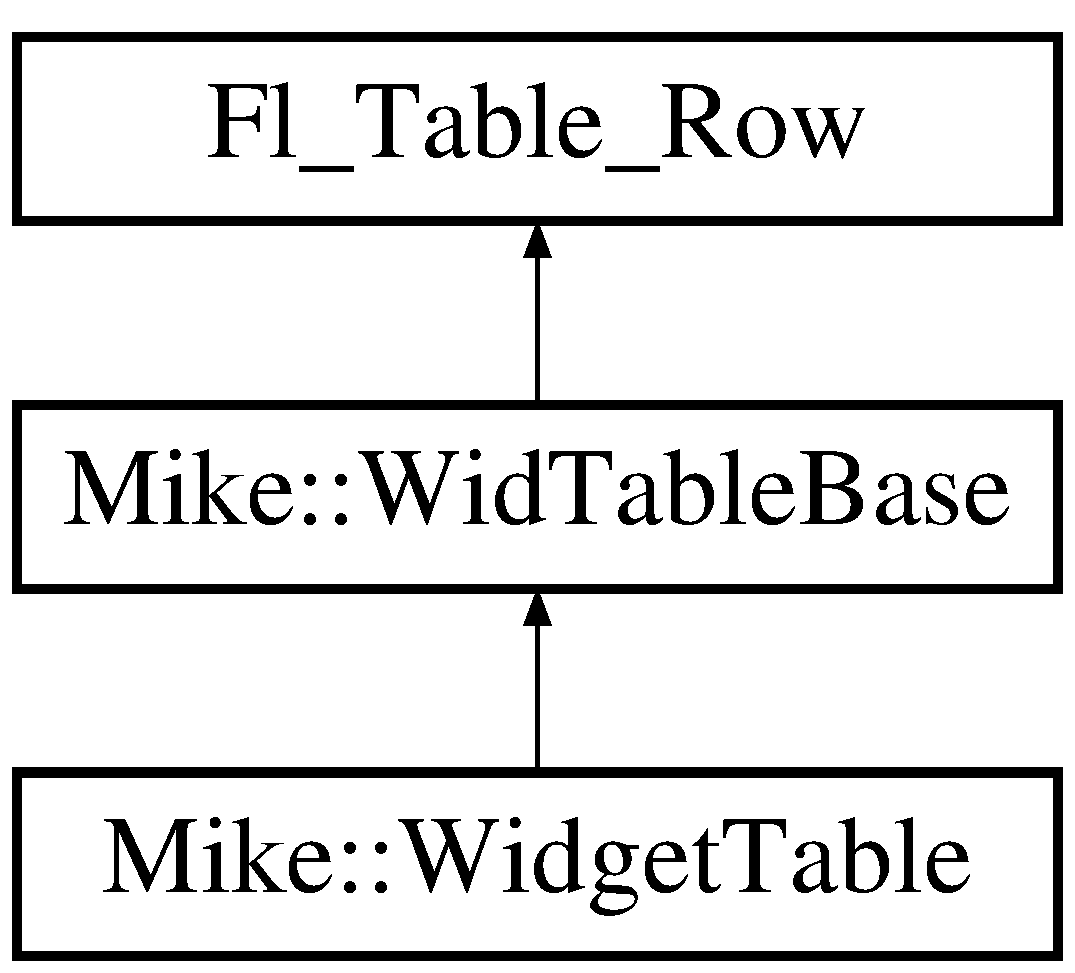
\includegraphics[height=3.000000cm]{class_mike_1_1_wid_table_base}
\end{center}
\end{figure}
\subsection*{Public Member Functions}
\begin{DoxyCompactItemize}
\item 
int \hyperlink{class_mike_1_1_wid_table_base_abdc666dec8fa95e8e6232c9eae6ee8e2}{Get\+Rows} ()
\item 
int \hyperlink{class_mike_1_1_wid_table_base_afac57108a679ea7b3800ab8a14e80209}{Get\+Cols} ()
\item 
int \hyperlink{class_mike_1_1_wid_table_base_ab9f884cfed7ee50f7037bf1e75258f11}{Get\+Top\+Row\+Price} ()
\item 
int \hyperlink{class_mike_1_1_wid_table_base_af29863e5a1695c64a748133b335ecc16}{Get\+Bottom\+Row\+Price} ()
\item 
void \hyperlink{class_mike_1_1_wid_table_base_a456b14469434d2fffe513a9d7cc39e25}{Set\+Top\+Row\+Price} (int value)
\item 
std\+::vector$<$ std\+::string $>$ $\ast$ \hyperlink{class_mike_1_1_wid_table_base_a8fab1137b438a8ae331c9ceeaae43acb}{Get\+Col\+Names} ()
\item 
int \hyperlink{class_mike_1_1_wid_table_base_a590a250d0bb443aef98a7250555d1c68}{Row\+Of\+Price} (long price)
\item 
long \hyperlink{class_mike_1_1_wid_table_base_afb5e90634ccda27eb8f40a1f2b6208a1}{Price\+Of\+Row} (int row)
\item 
virtual void \hyperlink{class_mike_1_1_wid_table_base_a71a0e404a020f7b8d10544113c16a4ce}{Set\+Columnn\+Width} (short width)
\end{DoxyCompactItemize}
\subsection*{Protected Member Functions}
\begin{DoxyCompactItemize}
\item 
\hyperlink{class_mike_1_1_wid_table_base_aa9d89f83f34c4ce8f0655ff3437374a5}{Wid\+Table\+Base} (int x, int y, int w, int h, const char $\ast$l)
\item 
\hyperlink{class_mike_1_1_wid_table_base_aa2cee360b485c40a08c556da54ffa439}{Wid\+Table\+Base} (int x, int y, int w, int h, const char $\ast$l, int top\+\_\+row\+\_\+price, int number\+\_\+rows=25, int number\+\_\+cols=15, int how\+\_\+many\+\_\+cols\+\_\+are\+\_\+buttons=5, std\+::vector$<$ std\+::string $>$ \hyperlink{class_mike_1_1_wid_table_base_acc76591b1fa97f8259fc95f492d8e1b9}{col\+\_\+names}=\{ \char`\"{}\char`\"{} \}, std\+::vector$<$ std\+::string $>$ button\+\_\+names=\{ \char`\"{}\char`\"{} \})
\item 
\hyperlink{class_mike_1_1_wid_table_base_a66c2828fd13a8abf4f5faa274e632542}{$\sim$\+Wid\+Table\+Base} ()
\item 
virtual void \hyperlink{class_mike_1_1_wid_table_base_aed65d79c6e84fd89abceaf6ffa079fad}{virt\+Button\+Cb} (Fl\+\_\+\+Widget $\ast$w, void $\ast$p)
\item 
void \hyperlink{class_mike_1_1_wid_table_base_a22ff7af61bac2dc33e596e68a236b845}{print\+In\+Table} (int row, int col, std\+::string text, Fl\+\_\+\+Color background\+Color=N\+U\+LL, Fl\+\_\+\+Color text\+Color=N\+U\+LL)
\item 
void \hyperlink{class_mike_1_1_wid_table_base_af7acb57a8144c9ab4e01a8300469b98e}{Clear\+Column} (int column)
\item 
void \hyperlink{class_mike_1_1_wid_table_base_a17021ef3e4cea06939284891dc27d61f}{Clear\+Row} (int row)
\item 
void \hyperlink{class_mike_1_1_wid_table_base_a4779181b9c1eebc13406f9093d665236}{clear\+All\+Button\+Labels} ()
\item 
virtual void \hyperlink{class_mike_1_1_wid_table_base_a980add59d3d60f68517b48a896e5eb3c}{Col\+Header\+Text} (char $\ast$s, int C)
\item 
void \hyperlink{class_mike_1_1_wid_table_base_a3486b3282392458231cb09f9d9a4e504}{Set\+Rows} (int num\+Rows)
\item 
void \hyperlink{class_mike_1_1_wid_table_base_a52555afc3c0f71ae166d862258303447}{Set\+Cols} (int num\+Col)
\item 
Fl\+\_\+\+Widget $\ast$ \hyperlink{class_mike_1_1_wid_table_base_a5c2de58aec7fa3751862b68f18031f88}{Get\+Element} (int n\+Row, int n\+Col)
\item 
void \hyperlink{class_mike_1_1_wid_table_base_a1a463c054dfd0dc563dedf0fbdaf3232}{draw\+\_\+cell} (Table\+Context context, int R=0, int C=0, int X=0, int Y=0, int W=0, int H=0)
\item 
void \hyperlink{class_mike_1_1_wid_table_base_a23f12c24def459d1dde1c53a7e237d4a}{Set\+Size} (int newrows, int newcols, \hyperlink{class_mike_1_1_wid_table_base}{Wid\+Table\+Base} $\ast$mytable, std\+::vector$<$ std\+::string $>$ button\+\_\+names=\{ \char`\"{}\char`\"{} \})
\end{DoxyCompactItemize}
\subsection*{Static Protected Member Functions}
\begin{DoxyCompactItemize}
\item 
static void \hyperlink{class_mike_1_1_wid_table_base_afba70372ad656f248ca4ea9dc408e41f}{button\+\_\+cb} (Fl\+\_\+\+Widget $\ast$w, void $\ast$p)
\end{DoxyCompactItemize}
\subsection*{Protected Attributes}
\begin{DoxyCompactItemize}
\item 
int \hyperlink{class_mike_1_1_wid_table_base_a72f42a61350eb88e259047217fe4d92f}{table\+\_\+rows}
\item 
int \hyperlink{class_mike_1_1_wid_table_base_a286d2c5a539c51110c59cbc3b5121d5b}{table\+\_\+cols}
\item 
int \hyperlink{class_mike_1_1_wid_table_base_a1f418b75c1d456ef2c167809edfa17db}{Button\+Cols\+Number}
\item 
int \hyperlink{class_mike_1_1_wid_table_base_a0b15be1c88a8a50bb65df9eb43027732}{Top\+Row\+Price}
\item 
short \hyperlink{class_mike_1_1_wid_table_base_a8821c66c2f042e78997e6f2b132b0b4d}{tabletype} = 0
\item 
std\+::vector$<$ std\+::string $>$ \hyperlink{class_mike_1_1_wid_table_base_acc76591b1fa97f8259fc95f492d8e1b9}{col\+\_\+names}
\item 
short \hyperlink{class_mike_1_1_wid_table_base_a610c3e633ae8fc7290881ffeda317475}{column\+Width} = 55
\end{DoxyCompactItemize}
\subsection*{Private Attributes}
\begin{DoxyCompactItemize}
\item 
std\+::stack$<$ Fl\+\_\+\+Input $\ast$ $>$ \hyperlink{class_mike_1_1_wid_table_base_a50bcff267ab19f59fa27bfb2264f815b}{shared\+Fl\+Input\+Pointers}
\end{DoxyCompactItemize}
\subsection*{Friends}
\begin{DoxyCompactItemize}
\item 
class \hyperlink{class_mike_1_1_wid_table_base_a3890cb6751c73d6d400ecb8ab17d7f2d}{Simple\+Table\+Window}
\end{DoxyCompactItemize}


\subsection{Constructor \& Destructor Documentation}
\mbox{\Hypertarget{class_mike_1_1_wid_table_base_aa9d89f83f34c4ce8f0655ff3437374a5}\label{class_mike_1_1_wid_table_base_aa9d89f83f34c4ce8f0655ff3437374a5}} 
\index{Mike\+::\+Wid\+Table\+Base@{Mike\+::\+Wid\+Table\+Base}!Wid\+Table\+Base@{Wid\+Table\+Base}}
\index{Wid\+Table\+Base@{Wid\+Table\+Base}!Mike\+::\+Wid\+Table\+Base@{Mike\+::\+Wid\+Table\+Base}}
\subsubsection{\texorpdfstring{Wid\+Table\+Base()}{WidTableBase()}\hspace{0.1cm}{\footnotesize\ttfamily [1/2]}}
{\footnotesize\ttfamily Mike\+::\+Wid\+Table\+Base\+::\+Wid\+Table\+Base (\begin{DoxyParamCaption}\item[{int}]{x,  }\item[{int}]{y,  }\item[{int}]{w,  }\item[{int}]{h,  }\item[{const char $\ast$}]{l }\end{DoxyParamCaption})\hspace{0.3cm}{\ttfamily [protected]}}

\mbox{\Hypertarget{class_mike_1_1_wid_table_base_aa2cee360b485c40a08c556da54ffa439}\label{class_mike_1_1_wid_table_base_aa2cee360b485c40a08c556da54ffa439}} 
\index{Mike\+::\+Wid\+Table\+Base@{Mike\+::\+Wid\+Table\+Base}!Wid\+Table\+Base@{Wid\+Table\+Base}}
\index{Wid\+Table\+Base@{Wid\+Table\+Base}!Mike\+::\+Wid\+Table\+Base@{Mike\+::\+Wid\+Table\+Base}}
\subsubsection{\texorpdfstring{Wid\+Table\+Base()}{WidTableBase()}\hspace{0.1cm}{\footnotesize\ttfamily [2/2]}}
{\footnotesize\ttfamily Mike\+::\+Wid\+Table\+Base\+::\+Wid\+Table\+Base (\begin{DoxyParamCaption}\item[{int}]{x,  }\item[{int}]{y,  }\item[{int}]{w,  }\item[{int}]{h,  }\item[{const char $\ast$}]{l,  }\item[{int}]{top\+\_\+row\+\_\+price,  }\item[{int}]{number\+\_\+rows = {\ttfamily 25},  }\item[{int}]{number\+\_\+cols = {\ttfamily 15},  }\item[{int}]{how\+\_\+many\+\_\+cols\+\_\+are\+\_\+buttons = {\ttfamily 5},  }\item[{std\+::vector$<$ std\+::string $>$}]{col\+\_\+names = {\ttfamily \{~\char`\"{}\char`\"{}~\}},  }\item[{std\+::vector$<$ std\+::string $>$}]{button\+\_\+names = {\ttfamily \{~\char`\"{}\char`\"{}~\}} }\end{DoxyParamCaption})\hspace{0.3cm}{\ttfamily [protected]}}

\mbox{\Hypertarget{class_mike_1_1_wid_table_base_a66c2828fd13a8abf4f5faa274e632542}\label{class_mike_1_1_wid_table_base_a66c2828fd13a8abf4f5faa274e632542}} 
\index{Mike\+::\+Wid\+Table\+Base@{Mike\+::\+Wid\+Table\+Base}!````~Wid\+Table\+Base@{$\sim$\+Wid\+Table\+Base}}
\index{````~Wid\+Table\+Base@{$\sim$\+Wid\+Table\+Base}!Mike\+::\+Wid\+Table\+Base@{Mike\+::\+Wid\+Table\+Base}}
\subsubsection{\texorpdfstring{$\sim$\+Wid\+Table\+Base()}{~WidTableBase()}}
{\footnotesize\ttfamily Mike\+::\+Wid\+Table\+Base\+::$\sim$\+Wid\+Table\+Base (\begin{DoxyParamCaption}{ }\end{DoxyParamCaption})\hspace{0.3cm}{\ttfamily [protected]}}



\subsection{Member Function Documentation}
\mbox{\Hypertarget{class_mike_1_1_wid_table_base_afba70372ad656f248ca4ea9dc408e41f}\label{class_mike_1_1_wid_table_base_afba70372ad656f248ca4ea9dc408e41f}} 
\index{Mike\+::\+Wid\+Table\+Base@{Mike\+::\+Wid\+Table\+Base}!button\+\_\+cb@{button\+\_\+cb}}
\index{button\+\_\+cb@{button\+\_\+cb}!Mike\+::\+Wid\+Table\+Base@{Mike\+::\+Wid\+Table\+Base}}
\subsubsection{\texorpdfstring{button\+\_\+cb()}{button\_cb()}}
{\footnotesize\ttfamily void Mike\+::\+Wid\+Table\+Base\+::button\+\_\+cb (\begin{DoxyParamCaption}\item[{Fl\+\_\+\+Widget $\ast$}]{w,  }\item[{void $\ast$}]{p }\end{DoxyParamCaption})\hspace{0.3cm}{\ttfamily [static]}, {\ttfamily [protected]}}

\mbox{\Hypertarget{class_mike_1_1_wid_table_base_a4779181b9c1eebc13406f9093d665236}\label{class_mike_1_1_wid_table_base_a4779181b9c1eebc13406f9093d665236}} 
\index{Mike\+::\+Wid\+Table\+Base@{Mike\+::\+Wid\+Table\+Base}!clear\+All\+Button\+Labels@{clear\+All\+Button\+Labels}}
\index{clear\+All\+Button\+Labels@{clear\+All\+Button\+Labels}!Mike\+::\+Wid\+Table\+Base@{Mike\+::\+Wid\+Table\+Base}}
\subsubsection{\texorpdfstring{clear\+All\+Button\+Labels()}{clearAllButtonLabels()}}
{\footnotesize\ttfamily void Mike\+::\+Wid\+Table\+Base\+::clear\+All\+Button\+Labels (\begin{DoxyParamCaption}{ }\end{DoxyParamCaption})\hspace{0.3cm}{\ttfamily [protected]}}

\mbox{\Hypertarget{class_mike_1_1_wid_table_base_af7acb57a8144c9ab4e01a8300469b98e}\label{class_mike_1_1_wid_table_base_af7acb57a8144c9ab4e01a8300469b98e}} 
\index{Mike\+::\+Wid\+Table\+Base@{Mike\+::\+Wid\+Table\+Base}!Clear\+Column@{Clear\+Column}}
\index{Clear\+Column@{Clear\+Column}!Mike\+::\+Wid\+Table\+Base@{Mike\+::\+Wid\+Table\+Base}}
\subsubsection{\texorpdfstring{Clear\+Column()}{ClearColumn()}}
{\footnotesize\ttfamily void Mike\+::\+Wid\+Table\+Base\+::\+Clear\+Column (\begin{DoxyParamCaption}\item[{int}]{column }\end{DoxyParamCaption})\hspace{0.3cm}{\ttfamily [protected]}}

\mbox{\Hypertarget{class_mike_1_1_wid_table_base_a17021ef3e4cea06939284891dc27d61f}\label{class_mike_1_1_wid_table_base_a17021ef3e4cea06939284891dc27d61f}} 
\index{Mike\+::\+Wid\+Table\+Base@{Mike\+::\+Wid\+Table\+Base}!Clear\+Row@{Clear\+Row}}
\index{Clear\+Row@{Clear\+Row}!Mike\+::\+Wid\+Table\+Base@{Mike\+::\+Wid\+Table\+Base}}
\subsubsection{\texorpdfstring{Clear\+Row()}{ClearRow()}}
{\footnotesize\ttfamily void Mike\+::\+Wid\+Table\+Base\+::\+Clear\+Row (\begin{DoxyParamCaption}\item[{int}]{row }\end{DoxyParamCaption})\hspace{0.3cm}{\ttfamily [protected]}}

\mbox{\Hypertarget{class_mike_1_1_wid_table_base_a980add59d3d60f68517b48a896e5eb3c}\label{class_mike_1_1_wid_table_base_a980add59d3d60f68517b48a896e5eb3c}} 
\index{Mike\+::\+Wid\+Table\+Base@{Mike\+::\+Wid\+Table\+Base}!Col\+Header\+Text@{Col\+Header\+Text}}
\index{Col\+Header\+Text@{Col\+Header\+Text}!Mike\+::\+Wid\+Table\+Base@{Mike\+::\+Wid\+Table\+Base}}
\subsubsection{\texorpdfstring{Col\+Header\+Text()}{ColHeaderText()}}
{\footnotesize\ttfamily void Mike\+::\+Wid\+Table\+Base\+::\+Col\+Header\+Text (\begin{DoxyParamCaption}\item[{char $\ast$}]{s,  }\item[{int}]{C }\end{DoxyParamCaption})\hspace{0.3cm}{\ttfamily [protected]}, {\ttfamily [virtual]}}

\mbox{\Hypertarget{class_mike_1_1_wid_table_base_a1a463c054dfd0dc563dedf0fbdaf3232}\label{class_mike_1_1_wid_table_base_a1a463c054dfd0dc563dedf0fbdaf3232}} 
\index{Mike\+::\+Wid\+Table\+Base@{Mike\+::\+Wid\+Table\+Base}!draw\+\_\+cell@{draw\+\_\+cell}}
\index{draw\+\_\+cell@{draw\+\_\+cell}!Mike\+::\+Wid\+Table\+Base@{Mike\+::\+Wid\+Table\+Base}}
\subsubsection{\texorpdfstring{draw\+\_\+cell()}{draw\_cell()}}
{\footnotesize\ttfamily void Mike\+::\+Wid\+Table\+Base\+::draw\+\_\+cell (\begin{DoxyParamCaption}\item[{Table\+Context}]{context,  }\item[{int}]{R = {\ttfamily 0},  }\item[{int}]{C = {\ttfamily 0},  }\item[{int}]{X = {\ttfamily 0},  }\item[{int}]{Y = {\ttfamily 0},  }\item[{int}]{W = {\ttfamily 0},  }\item[{int}]{H = {\ttfamily 0} }\end{DoxyParamCaption})\hspace{0.3cm}{\ttfamily [protected]}}

\mbox{\Hypertarget{class_mike_1_1_wid_table_base_af29863e5a1695c64a748133b335ecc16}\label{class_mike_1_1_wid_table_base_af29863e5a1695c64a748133b335ecc16}} 
\index{Mike\+::\+Wid\+Table\+Base@{Mike\+::\+Wid\+Table\+Base}!Get\+Bottom\+Row\+Price@{Get\+Bottom\+Row\+Price}}
\index{Get\+Bottom\+Row\+Price@{Get\+Bottom\+Row\+Price}!Mike\+::\+Wid\+Table\+Base@{Mike\+::\+Wid\+Table\+Base}}
\subsubsection{\texorpdfstring{Get\+Bottom\+Row\+Price()}{GetBottomRowPrice()}}
{\footnotesize\ttfamily int Mike\+::\+Wid\+Table\+Base\+::\+Get\+Bottom\+Row\+Price (\begin{DoxyParamCaption}{ }\end{DoxyParamCaption})\hspace{0.3cm}{\ttfamily [inline]}}

\mbox{\Hypertarget{class_mike_1_1_wid_table_base_a8fab1137b438a8ae331c9ceeaae43acb}\label{class_mike_1_1_wid_table_base_a8fab1137b438a8ae331c9ceeaae43acb}} 
\index{Mike\+::\+Wid\+Table\+Base@{Mike\+::\+Wid\+Table\+Base}!Get\+Col\+Names@{Get\+Col\+Names}}
\index{Get\+Col\+Names@{Get\+Col\+Names}!Mike\+::\+Wid\+Table\+Base@{Mike\+::\+Wid\+Table\+Base}}
\subsubsection{\texorpdfstring{Get\+Col\+Names()}{GetColNames()}}
{\footnotesize\ttfamily std\+::vector$<$std\+::string$>$$\ast$ Mike\+::\+Wid\+Table\+Base\+::\+Get\+Col\+Names (\begin{DoxyParamCaption}{ }\end{DoxyParamCaption})\hspace{0.3cm}{\ttfamily [inline]}}

\mbox{\Hypertarget{class_mike_1_1_wid_table_base_afac57108a679ea7b3800ab8a14e80209}\label{class_mike_1_1_wid_table_base_afac57108a679ea7b3800ab8a14e80209}} 
\index{Mike\+::\+Wid\+Table\+Base@{Mike\+::\+Wid\+Table\+Base}!Get\+Cols@{Get\+Cols}}
\index{Get\+Cols@{Get\+Cols}!Mike\+::\+Wid\+Table\+Base@{Mike\+::\+Wid\+Table\+Base}}
\subsubsection{\texorpdfstring{Get\+Cols()}{GetCols()}}
{\footnotesize\ttfamily int Mike\+::\+Wid\+Table\+Base\+::\+Get\+Cols (\begin{DoxyParamCaption}{ }\end{DoxyParamCaption})\hspace{0.3cm}{\ttfamily [inline]}}

\mbox{\Hypertarget{class_mike_1_1_wid_table_base_a5c2de58aec7fa3751862b68f18031f88}\label{class_mike_1_1_wid_table_base_a5c2de58aec7fa3751862b68f18031f88}} 
\index{Mike\+::\+Wid\+Table\+Base@{Mike\+::\+Wid\+Table\+Base}!Get\+Element@{Get\+Element}}
\index{Get\+Element@{Get\+Element}!Mike\+::\+Wid\+Table\+Base@{Mike\+::\+Wid\+Table\+Base}}
\subsubsection{\texorpdfstring{Get\+Element()}{GetElement()}}
{\footnotesize\ttfamily Fl\+\_\+\+Widget $\ast$ Mike\+::\+Wid\+Table\+Base\+::\+Get\+Element (\begin{DoxyParamCaption}\item[{int}]{n\+Row,  }\item[{int}]{n\+Col }\end{DoxyParamCaption})\hspace{0.3cm}{\ttfamily [protected]}}

\mbox{\Hypertarget{class_mike_1_1_wid_table_base_abdc666dec8fa95e8e6232c9eae6ee8e2}\label{class_mike_1_1_wid_table_base_abdc666dec8fa95e8e6232c9eae6ee8e2}} 
\index{Mike\+::\+Wid\+Table\+Base@{Mike\+::\+Wid\+Table\+Base}!Get\+Rows@{Get\+Rows}}
\index{Get\+Rows@{Get\+Rows}!Mike\+::\+Wid\+Table\+Base@{Mike\+::\+Wid\+Table\+Base}}
\subsubsection{\texorpdfstring{Get\+Rows()}{GetRows()}}
{\footnotesize\ttfamily int Mike\+::\+Wid\+Table\+Base\+::\+Get\+Rows (\begin{DoxyParamCaption}{ }\end{DoxyParamCaption})\hspace{0.3cm}{\ttfamily [inline]}}

\mbox{\Hypertarget{class_mike_1_1_wid_table_base_ab9f884cfed7ee50f7037bf1e75258f11}\label{class_mike_1_1_wid_table_base_ab9f884cfed7ee50f7037bf1e75258f11}} 
\index{Mike\+::\+Wid\+Table\+Base@{Mike\+::\+Wid\+Table\+Base}!Get\+Top\+Row\+Price@{Get\+Top\+Row\+Price}}
\index{Get\+Top\+Row\+Price@{Get\+Top\+Row\+Price}!Mike\+::\+Wid\+Table\+Base@{Mike\+::\+Wid\+Table\+Base}}
\subsubsection{\texorpdfstring{Get\+Top\+Row\+Price()}{GetTopRowPrice()}}
{\footnotesize\ttfamily int Mike\+::\+Wid\+Table\+Base\+::\+Get\+Top\+Row\+Price (\begin{DoxyParamCaption}{ }\end{DoxyParamCaption})\hspace{0.3cm}{\ttfamily [inline]}}

\mbox{\Hypertarget{class_mike_1_1_wid_table_base_afb5e90634ccda27eb8f40a1f2b6208a1}\label{class_mike_1_1_wid_table_base_afb5e90634ccda27eb8f40a1f2b6208a1}} 
\index{Mike\+::\+Wid\+Table\+Base@{Mike\+::\+Wid\+Table\+Base}!Price\+Of\+Row@{Price\+Of\+Row}}
\index{Price\+Of\+Row@{Price\+Of\+Row}!Mike\+::\+Wid\+Table\+Base@{Mike\+::\+Wid\+Table\+Base}}
\subsubsection{\texorpdfstring{Price\+Of\+Row()}{PriceOfRow()}}
{\footnotesize\ttfamily long Mike\+::\+Wid\+Table\+Base\+::\+Price\+Of\+Row (\begin{DoxyParamCaption}\item[{int}]{row }\end{DoxyParamCaption})}

\mbox{\Hypertarget{class_mike_1_1_wid_table_base_a22ff7af61bac2dc33e596e68a236b845}\label{class_mike_1_1_wid_table_base_a22ff7af61bac2dc33e596e68a236b845}} 
\index{Mike\+::\+Wid\+Table\+Base@{Mike\+::\+Wid\+Table\+Base}!print\+In\+Table@{print\+In\+Table}}
\index{print\+In\+Table@{print\+In\+Table}!Mike\+::\+Wid\+Table\+Base@{Mike\+::\+Wid\+Table\+Base}}
\subsubsection{\texorpdfstring{print\+In\+Table()}{printInTable()}}
{\footnotesize\ttfamily void Mike\+::\+Wid\+Table\+Base\+::print\+In\+Table (\begin{DoxyParamCaption}\item[{int}]{row,  }\item[{int}]{col,  }\item[{std\+::string}]{text,  }\item[{Fl\+\_\+\+Color}]{background\+Color = {\ttfamily NULL},  }\item[{Fl\+\_\+\+Color}]{text\+Color = {\ttfamily NULL} }\end{DoxyParamCaption})\hspace{0.3cm}{\ttfamily [protected]}}

\mbox{\Hypertarget{class_mike_1_1_wid_table_base_a590a250d0bb443aef98a7250555d1c68}\label{class_mike_1_1_wid_table_base_a590a250d0bb443aef98a7250555d1c68}} 
\index{Mike\+::\+Wid\+Table\+Base@{Mike\+::\+Wid\+Table\+Base}!Row\+Of\+Price@{Row\+Of\+Price}}
\index{Row\+Of\+Price@{Row\+Of\+Price}!Mike\+::\+Wid\+Table\+Base@{Mike\+::\+Wid\+Table\+Base}}
\subsubsection{\texorpdfstring{Row\+Of\+Price()}{RowOfPrice()}}
{\footnotesize\ttfamily int Mike\+::\+Wid\+Table\+Base\+::\+Row\+Of\+Price (\begin{DoxyParamCaption}\item[{long}]{price }\end{DoxyParamCaption})}

\mbox{\Hypertarget{class_mike_1_1_wid_table_base_a52555afc3c0f71ae166d862258303447}\label{class_mike_1_1_wid_table_base_a52555afc3c0f71ae166d862258303447}} 
\index{Mike\+::\+Wid\+Table\+Base@{Mike\+::\+Wid\+Table\+Base}!Set\+Cols@{Set\+Cols}}
\index{Set\+Cols@{Set\+Cols}!Mike\+::\+Wid\+Table\+Base@{Mike\+::\+Wid\+Table\+Base}}
\subsubsection{\texorpdfstring{Set\+Cols()}{SetCols()}}
{\footnotesize\ttfamily void Mike\+::\+Wid\+Table\+Base\+::\+Set\+Cols (\begin{DoxyParamCaption}\item[{int}]{num\+Col }\end{DoxyParamCaption})\hspace{0.3cm}{\ttfamily [inline]}, {\ttfamily [protected]}}

\mbox{\Hypertarget{class_mike_1_1_wid_table_base_a71a0e404a020f7b8d10544113c16a4ce}\label{class_mike_1_1_wid_table_base_a71a0e404a020f7b8d10544113c16a4ce}} 
\index{Mike\+::\+Wid\+Table\+Base@{Mike\+::\+Wid\+Table\+Base}!Set\+Columnn\+Width@{Set\+Columnn\+Width}}
\index{Set\+Columnn\+Width@{Set\+Columnn\+Width}!Mike\+::\+Wid\+Table\+Base@{Mike\+::\+Wid\+Table\+Base}}
\subsubsection{\texorpdfstring{Set\+Columnn\+Width()}{SetColumnnWidth()}}
{\footnotesize\ttfamily virtual void Mike\+::\+Wid\+Table\+Base\+::\+Set\+Columnn\+Width (\begin{DoxyParamCaption}\item[{short}]{width }\end{DoxyParamCaption})\hspace{0.3cm}{\ttfamily [inline]}, {\ttfamily [virtual]}}

\mbox{\Hypertarget{class_mike_1_1_wid_table_base_a3486b3282392458231cb09f9d9a4e504}\label{class_mike_1_1_wid_table_base_a3486b3282392458231cb09f9d9a4e504}} 
\index{Mike\+::\+Wid\+Table\+Base@{Mike\+::\+Wid\+Table\+Base}!Set\+Rows@{Set\+Rows}}
\index{Set\+Rows@{Set\+Rows}!Mike\+::\+Wid\+Table\+Base@{Mike\+::\+Wid\+Table\+Base}}
\subsubsection{\texorpdfstring{Set\+Rows()}{SetRows()}}
{\footnotesize\ttfamily void Mike\+::\+Wid\+Table\+Base\+::\+Set\+Rows (\begin{DoxyParamCaption}\item[{int}]{num\+Rows }\end{DoxyParamCaption})\hspace{0.3cm}{\ttfamily [inline]}, {\ttfamily [protected]}}

\mbox{\Hypertarget{class_mike_1_1_wid_table_base_a23f12c24def459d1dde1c53a7e237d4a}\label{class_mike_1_1_wid_table_base_a23f12c24def459d1dde1c53a7e237d4a}} 
\index{Mike\+::\+Wid\+Table\+Base@{Mike\+::\+Wid\+Table\+Base}!Set\+Size@{Set\+Size}}
\index{Set\+Size@{Set\+Size}!Mike\+::\+Wid\+Table\+Base@{Mike\+::\+Wid\+Table\+Base}}
\subsubsection{\texorpdfstring{Set\+Size()}{SetSize()}}
{\footnotesize\ttfamily void Mike\+::\+Wid\+Table\+Base\+::\+Set\+Size (\begin{DoxyParamCaption}\item[{int}]{newrows,  }\item[{int}]{newcols,  }\item[{\hyperlink{class_mike_1_1_wid_table_base}{Wid\+Table\+Base} $\ast$}]{mytable,  }\item[{std\+::vector$<$ std\+::string $>$}]{button\+\_\+names = {\ttfamily \{~\char`\"{}\char`\"{}~\}} }\end{DoxyParamCaption})\hspace{0.3cm}{\ttfamily [protected]}}

\mbox{\Hypertarget{class_mike_1_1_wid_table_base_a456b14469434d2fffe513a9d7cc39e25}\label{class_mike_1_1_wid_table_base_a456b14469434d2fffe513a9d7cc39e25}} 
\index{Mike\+::\+Wid\+Table\+Base@{Mike\+::\+Wid\+Table\+Base}!Set\+Top\+Row\+Price@{Set\+Top\+Row\+Price}}
\index{Set\+Top\+Row\+Price@{Set\+Top\+Row\+Price}!Mike\+::\+Wid\+Table\+Base@{Mike\+::\+Wid\+Table\+Base}}
\subsubsection{\texorpdfstring{Set\+Top\+Row\+Price()}{SetTopRowPrice()}}
{\footnotesize\ttfamily void Mike\+::\+Wid\+Table\+Base\+::\+Set\+Top\+Row\+Price (\begin{DoxyParamCaption}\item[{int}]{value }\end{DoxyParamCaption})\hspace{0.3cm}{\ttfamily [inline]}}

\mbox{\Hypertarget{class_mike_1_1_wid_table_base_aed65d79c6e84fd89abceaf6ffa079fad}\label{class_mike_1_1_wid_table_base_aed65d79c6e84fd89abceaf6ffa079fad}} 
\index{Mike\+::\+Wid\+Table\+Base@{Mike\+::\+Wid\+Table\+Base}!virt\+Button\+Cb@{virt\+Button\+Cb}}
\index{virt\+Button\+Cb@{virt\+Button\+Cb}!Mike\+::\+Wid\+Table\+Base@{Mike\+::\+Wid\+Table\+Base}}
\subsubsection{\texorpdfstring{virt\+Button\+Cb()}{virtButtonCb()}}
{\footnotesize\ttfamily virtual void Mike\+::\+Wid\+Table\+Base\+::virt\+Button\+Cb (\begin{DoxyParamCaption}\item[{Fl\+\_\+\+Widget $\ast$}]{w,  }\item[{void $\ast$}]{p }\end{DoxyParamCaption})\hspace{0.3cm}{\ttfamily [inline]}, {\ttfamily [protected]}, {\ttfamily [virtual]}}



Reimplemented in \hyperlink{class_mike_1_1_widget_table_affddec39940626f7d72ffaf9e02d04e4}{Mike\+::\+Widget\+Table}.



\subsection{Friends And Related Function Documentation}
\mbox{\Hypertarget{class_mike_1_1_wid_table_base_a3890cb6751c73d6d400ecb8ab17d7f2d}\label{class_mike_1_1_wid_table_base_a3890cb6751c73d6d400ecb8ab17d7f2d}} 
\index{Mike\+::\+Wid\+Table\+Base@{Mike\+::\+Wid\+Table\+Base}!Simple\+Table\+Window@{Simple\+Table\+Window}}
\index{Simple\+Table\+Window@{Simple\+Table\+Window}!Mike\+::\+Wid\+Table\+Base@{Mike\+::\+Wid\+Table\+Base}}
\subsubsection{\texorpdfstring{Simple\+Table\+Window}{SimpleTableWindow}}
{\footnotesize\ttfamily friend class Simple\+Table\+Window\hspace{0.3cm}{\ttfamily [friend]}}



\subsection{Member Data Documentation}
\mbox{\Hypertarget{class_mike_1_1_wid_table_base_a1f418b75c1d456ef2c167809edfa17db}\label{class_mike_1_1_wid_table_base_a1f418b75c1d456ef2c167809edfa17db}} 
\index{Mike\+::\+Wid\+Table\+Base@{Mike\+::\+Wid\+Table\+Base}!Button\+Cols\+Number@{Button\+Cols\+Number}}
\index{Button\+Cols\+Number@{Button\+Cols\+Number}!Mike\+::\+Wid\+Table\+Base@{Mike\+::\+Wid\+Table\+Base}}
\subsubsection{\texorpdfstring{Button\+Cols\+Number}{ButtonColsNumber}}
{\footnotesize\ttfamily int Mike\+::\+Wid\+Table\+Base\+::\+Button\+Cols\+Number\hspace{0.3cm}{\ttfamily [protected]}}

\mbox{\Hypertarget{class_mike_1_1_wid_table_base_acc76591b1fa97f8259fc95f492d8e1b9}\label{class_mike_1_1_wid_table_base_acc76591b1fa97f8259fc95f492d8e1b9}} 
\index{Mike\+::\+Wid\+Table\+Base@{Mike\+::\+Wid\+Table\+Base}!col\+\_\+names@{col\+\_\+names}}
\index{col\+\_\+names@{col\+\_\+names}!Mike\+::\+Wid\+Table\+Base@{Mike\+::\+Wid\+Table\+Base}}
\subsubsection{\texorpdfstring{col\+\_\+names}{col\_names}}
{\footnotesize\ttfamily std\+::vector$<$std\+::string$>$ Mike\+::\+Wid\+Table\+Base\+::col\+\_\+names\hspace{0.3cm}{\ttfamily [protected]}}

\mbox{\Hypertarget{class_mike_1_1_wid_table_base_a610c3e633ae8fc7290881ffeda317475}\label{class_mike_1_1_wid_table_base_a610c3e633ae8fc7290881ffeda317475}} 
\index{Mike\+::\+Wid\+Table\+Base@{Mike\+::\+Wid\+Table\+Base}!column\+Width@{column\+Width}}
\index{column\+Width@{column\+Width}!Mike\+::\+Wid\+Table\+Base@{Mike\+::\+Wid\+Table\+Base}}
\subsubsection{\texorpdfstring{column\+Width}{columnWidth}}
{\footnotesize\ttfamily short Mike\+::\+Wid\+Table\+Base\+::column\+Width = 55\hspace{0.3cm}{\ttfamily [protected]}}

\mbox{\Hypertarget{class_mike_1_1_wid_table_base_a50bcff267ab19f59fa27bfb2264f815b}\label{class_mike_1_1_wid_table_base_a50bcff267ab19f59fa27bfb2264f815b}} 
\index{Mike\+::\+Wid\+Table\+Base@{Mike\+::\+Wid\+Table\+Base}!shared\+Fl\+Input\+Pointers@{shared\+Fl\+Input\+Pointers}}
\index{shared\+Fl\+Input\+Pointers@{shared\+Fl\+Input\+Pointers}!Mike\+::\+Wid\+Table\+Base@{Mike\+::\+Wid\+Table\+Base}}
\subsubsection{\texorpdfstring{shared\+Fl\+Input\+Pointers}{sharedFlInputPointers}}
{\footnotesize\ttfamily std\+::stack$<$Fl\+\_\+\+Input$\ast$$>$ Mike\+::\+Wid\+Table\+Base\+::shared\+Fl\+Input\+Pointers\hspace{0.3cm}{\ttfamily [private]}}

\mbox{\Hypertarget{class_mike_1_1_wid_table_base_a286d2c5a539c51110c59cbc3b5121d5b}\label{class_mike_1_1_wid_table_base_a286d2c5a539c51110c59cbc3b5121d5b}} 
\index{Mike\+::\+Wid\+Table\+Base@{Mike\+::\+Wid\+Table\+Base}!table\+\_\+cols@{table\+\_\+cols}}
\index{table\+\_\+cols@{table\+\_\+cols}!Mike\+::\+Wid\+Table\+Base@{Mike\+::\+Wid\+Table\+Base}}
\subsubsection{\texorpdfstring{table\+\_\+cols}{table\_cols}}
{\footnotesize\ttfamily int Mike\+::\+Wid\+Table\+Base\+::table\+\_\+cols\hspace{0.3cm}{\ttfamily [protected]}}

\mbox{\Hypertarget{class_mike_1_1_wid_table_base_a72f42a61350eb88e259047217fe4d92f}\label{class_mike_1_1_wid_table_base_a72f42a61350eb88e259047217fe4d92f}} 
\index{Mike\+::\+Wid\+Table\+Base@{Mike\+::\+Wid\+Table\+Base}!table\+\_\+rows@{table\+\_\+rows}}
\index{table\+\_\+rows@{table\+\_\+rows}!Mike\+::\+Wid\+Table\+Base@{Mike\+::\+Wid\+Table\+Base}}
\subsubsection{\texorpdfstring{table\+\_\+rows}{table\_rows}}
{\footnotesize\ttfamily int Mike\+::\+Wid\+Table\+Base\+::table\+\_\+rows\hspace{0.3cm}{\ttfamily [protected]}}

\mbox{\Hypertarget{class_mike_1_1_wid_table_base_a8821c66c2f042e78997e6f2b132b0b4d}\label{class_mike_1_1_wid_table_base_a8821c66c2f042e78997e6f2b132b0b4d}} 
\index{Mike\+::\+Wid\+Table\+Base@{Mike\+::\+Wid\+Table\+Base}!tabletype@{tabletype}}
\index{tabletype@{tabletype}!Mike\+::\+Wid\+Table\+Base@{Mike\+::\+Wid\+Table\+Base}}
\subsubsection{\texorpdfstring{tabletype}{tabletype}}
{\footnotesize\ttfamily short Mike\+::\+Wid\+Table\+Base\+::tabletype = 0\hspace{0.3cm}{\ttfamily [protected]}}

\mbox{\Hypertarget{class_mike_1_1_wid_table_base_a0b15be1c88a8a50bb65df9eb43027732}\label{class_mike_1_1_wid_table_base_a0b15be1c88a8a50bb65df9eb43027732}} 
\index{Mike\+::\+Wid\+Table\+Base@{Mike\+::\+Wid\+Table\+Base}!Top\+Row\+Price@{Top\+Row\+Price}}
\index{Top\+Row\+Price@{Top\+Row\+Price}!Mike\+::\+Wid\+Table\+Base@{Mike\+::\+Wid\+Table\+Base}}
\subsubsection{\texorpdfstring{Top\+Row\+Price}{TopRowPrice}}
{\footnotesize\ttfamily int Mike\+::\+Wid\+Table\+Base\+::\+Top\+Row\+Price\hspace{0.3cm}{\ttfamily [protected]}}



The documentation for this class was generated from the following files\+:\begin{DoxyCompactItemize}
\item 
src/work\+In\+Progress/\hyperlink{_wid_table_base_8h}{Wid\+Table\+Base.\+h}\item 
src/work\+In\+Progress/\hyperlink{_wid_table_base_8cpp}{Wid\+Table\+Base.\+cpp}\end{DoxyCompactItemize}

\chapter{File Documentation}
\hypertarget{_control_8cpp}{}\section{src/\+Control.cpp File Reference}
\label{_control_8cpp}\index{src/\+Control.\+cpp@{src/\+Control.\+cpp}}
{\ttfamily \#include \char`\"{}Control.\+h\char`\"{}}\newline
{\ttfamily \#include $<$iostream$>$}\newline
\subsection*{Namespaces}
\begin{DoxyCompactItemize}
\item 
 \hyperlink{namespace_mike}{Mike}
\end{DoxyCompactItemize}
\subsection*{Functions}
\begin{DoxyCompactItemize}
\item 
int \hyperlink{namespace_mike_ada7afe897748f668730c74456952e356}{Mike\+::frequency\+\_\+of\+\_\+primes} (int n)
\end{DoxyCompactItemize}

\hypertarget{_control_8h}{}\section{src/\+Control.h File Reference}
\label{_control_8h}\index{src/\+Control.\+h@{src/\+Control.\+h}}
{\ttfamily \#include \char`\"{}Fluid\+Price\+Control.\+h\char`\"{}}\newline
\subsection*{Classes}
\begin{DoxyCompactItemize}
\item 
class \hyperlink{class_mike_1_1_control}{Mike\+::\+Control}
\end{DoxyCompactItemize}
\subsection*{Namespaces}
\begin{DoxyCompactItemize}
\item 
 \hyperlink{namespace_mike}{Mike}
\end{DoxyCompactItemize}

\hypertarget{_data_8cpp}{}\section{src/\+Data.cpp File Reference}
\label{_data_8cpp}\index{src/\+Data.\+cpp@{src/\+Data.\+cpp}}
{\ttfamily \#include \char`\"{}Data.\+h\char`\"{}}\newline
\subsection*{Namespaces}
\begin{DoxyCompactItemize}
\item 
 \hyperlink{namespace_mike}{Mike}
\end{DoxyCompactItemize}

\hypertarget{_data_8h}{}\section{src/\+Data.h File Reference}
\label{_data_8h}\index{src/\+Data.\+h@{src/\+Data.\+h}}
{\ttfamily \#include \char`\"{}F\+L\+U\+I\+D\textbackslash{}\+Fluid\+Price\+Control.\+h\char`\"{}}\newline
\subsection*{Classes}
\begin{DoxyCompactItemize}
\item 
struct \hyperlink{struct_mike_1_1_data_u_i_event}{Mike\+::\+Data\+U\+I\+Event}
\item 
class \hyperlink{class_mike_1_1_data_u_i}{Mike\+::\+Data\+UI}
\item 
class \hyperlink{class_mike_1_1_data}{Mike\+::\+Data}
\end{DoxyCompactItemize}
\subsection*{Namespaces}
\begin{DoxyCompactItemize}
\item 
 \hyperlink{namespace_mike}{Mike}
\end{DoxyCompactItemize}
\subsection*{Enumerations}
\begin{DoxyCompactItemize}
\item 
enum \hyperlink{namespace_mike_ac75044494e0b43141b5cefbcd63b7dde}{Mike\+::\+Data\+U\+I\+Button} \{ \hyperlink{namespace_mike_ac75044494e0b43141b5cefbcd63b7ddeafe84ab8fffe0adb5a7f80f7fc92b3eac}{Mike\+::\+Data\+U\+I\+Button\+::\+U\+P\+B\+TN}, 
\hyperlink{namespace_mike_ac75044494e0b43141b5cefbcd63b7ddea276c9b2cc5f83e23e8a6207ce8453f41}{Mike\+::\+Data\+U\+I\+Button\+::\+D\+W\+N\+B\+TN}, 
\hyperlink{namespace_mike_ac75044494e0b43141b5cefbcd63b7ddea3c93f85078b290625b7c4db299979c4f}{Mike\+::\+Data\+U\+I\+Button\+::\+S\+L\+I\+D\+ER}, 
\hyperlink{namespace_mike_ac75044494e0b43141b5cefbcd63b7ddeaba2b45bdc11e2a4a6e86aab2ac693cbb}{Mike\+::\+Data\+U\+I\+Button\+::\+E\+M\+P\+TY}
 \}
\end{DoxyCompactItemize}

\hypertarget{_fluid_control_interface_8cxx}{}\section{src/\+F\+L\+U\+I\+D/\+Fluid\+Control\+Interface.cxx File Reference}
\label{_fluid_control_interface_8cxx}\index{src/\+F\+L\+U\+I\+D/\+Fluid\+Control\+Interface.\+cxx@{src/\+F\+L\+U\+I\+D/\+Fluid\+Control\+Interface.\+cxx}}
{\ttfamily \#include \char`\"{}Fluid\+Control\+Interface.\+h\char`\"{}}\newline

\hypertarget{_fluid_control_interface_8h}{}\section{F\+L\+U\+I\+D/\+Fluid\+Control\+Interface.h File Reference}
\label{_fluid_control_interface_8h}\index{F\+L\+U\+I\+D/\+Fluid\+Control\+Interface.\+h@{F\+L\+U\+I\+D/\+Fluid\+Control\+Interface.\+h}}
{\ttfamily \#include $<$F\+L/\+Fl.\+H$>$}\newline
{\ttfamily \#include $<$F\+L/\+Fl\+\_\+\+Double\+\_\+\+Window.\+H$>$}\newline
{\ttfamily \#include $<$F\+L/\+Fl\+\_\+\+Button.\+H$>$}\newline
{\ttfamily \#include $<$F\+L/\+Fl\+\_\+\+Box.\+H$>$}\newline
\subsection*{Classes}
\begin{DoxyCompactItemize}
\item 
class \hyperlink{class_fluid_control_interface}{Fluid\+Control\+Interface}
\end{DoxyCompactItemize}

\hypertarget{_fluid_interface_8cxx}{}\section{src/\+F\+L\+U\+I\+D/\+Fluid\+Interface.cxx File Reference}
\label{_fluid_interface_8cxx}\index{src/\+F\+L\+U\+I\+D/\+Fluid\+Interface.\+cxx@{src/\+F\+L\+U\+I\+D/\+Fluid\+Interface.\+cxx}}
{\ttfamily \#include \char`\"{}Fluid\+Interface.\+h\char`\"{}}\newline

\hypertarget{_fluid_interface_8h}{}\section{src/\+F\+L\+U\+I\+D/\+Fluid\+Interface.h File Reference}
\label{_fluid_interface_8h}\index{src/\+F\+L\+U\+I\+D/\+Fluid\+Interface.\+h@{src/\+F\+L\+U\+I\+D/\+Fluid\+Interface.\+h}}
{\ttfamily \#include $<$F\+L/\+Fl.\+H$>$}\newline
{\ttfamily \#include $<$F\+L/\+Fl\+\_\+\+Double\+\_\+\+Window.\+H$>$}\newline
{\ttfamily \#include $<$F\+L/\+Fl\+\_\+\+Value\+\_\+\+Input.\+H$>$}\newline
{\ttfamily \#include $<$F\+L/\+Fl\+\_\+\+Table.\+H$>$}\newline
{\ttfamily \#include $<$F\+L/\+Fl\+\_\+\+Button.\+H$>$}\newline
{\ttfamily \#include $<$F\+L/\+Fl\+\_\+\+Output.\+H$>$}\newline
\subsection*{Classes}
\begin{DoxyCompactItemize}
\item 
class \hyperlink{class_fluid_interface}{Fluid\+Interface}
\end{DoxyCompactItemize}

\hypertarget{_fluid_price_control_8cxx}{}\section{F\+L\+U\+I\+D/\+Fluid\+Price\+Control.cxx File Reference}
\label{_fluid_price_control_8cxx}\index{F\+L\+U\+I\+D/\+Fluid\+Price\+Control.\+cxx@{F\+L\+U\+I\+D/\+Fluid\+Price\+Control.\+cxx}}
{\ttfamily \#include \char`\"{}Fluid\+Price\+Control.\+h\char`\"{}}\newline

\hypertarget{_fluid_price_control_8h}{}\section{src/\+F\+L\+U\+I\+D/\+Fluid\+Price\+Control.h File Reference}
\label{_fluid_price_control_8h}\index{src/\+F\+L\+U\+I\+D/\+Fluid\+Price\+Control.\+h@{src/\+F\+L\+U\+I\+D/\+Fluid\+Price\+Control.\+h}}
{\ttfamily \#include $<$F\+L/\+Fl.\+H$>$}\newline
{\ttfamily \#include $<$F\+L/\+Fl\+\_\+\+Double\+\_\+\+Window.\+H$>$}\newline
{\ttfamily \#include $<$F\+L/\+Fl\+\_\+\+Button.\+H$>$}\newline
{\ttfamily \#include $<$F\+L/\+Fl\+\_\+\+Output.\+H$>$}\newline
{\ttfamily \#include $<$F\+L/\+Fl\+\_\+\+Value\+\_\+\+Slider.\+H$>$}\newline
\subsection*{Classes}
\begin{DoxyCompactItemize}
\item 
class \hyperlink{class_fluid_price_control_u_i}{Fluid\+Price\+Control\+UI}
\end{DoxyCompactItemize}

\hypertarget{_mike_u_i_8h}{}\section{src/\+F\+L\+U\+I\+D/\+Mike\+UI.h File Reference}
\label{_mike_u_i_8h}\index{src/\+F\+L\+U\+I\+D/\+Mike\+U\+I.\+h@{src/\+F\+L\+U\+I\+D/\+Mike\+U\+I.\+h}}
\subsection*{Classes}
\begin{DoxyCompactItemize}
\item 
class \hyperlink{class_mike_u_i}{Mike\+UI}
\end{DoxyCompactItemize}

\hypertarget{main_8cpp}{}\section{src/main.cpp File Reference}
\label{main_8cpp}\index{src/main.\+cpp@{src/main.\+cpp}}
{\ttfamily \#include $<$iostream$>$}\newline
{\ttfamily \#include \char`\"{}F\+L\textbackslash{}\+Fl.\+H\char`\"{}}\newline
{\ttfamily \#include \char`\"{}Control.\+h\char`\"{}}\newline
\subsection*{Namespaces}
\begin{DoxyCompactItemize}
\item 
 \hyperlink{namespace_mike}{Mike}
\end{DoxyCompactItemize}
\subsection*{Functions}
\begin{DoxyCompactItemize}
\item 
int \hyperlink{main_8cpp_ae66f6b31b5ad750f1fe042a706a4e3d4}{main} ()
\end{DoxyCompactItemize}


\subsection{Function Documentation}
\mbox{\Hypertarget{main_8cpp_ae66f6b31b5ad750f1fe042a706a4e3d4}\label{main_8cpp_ae66f6b31b5ad750f1fe042a706a4e3d4}} 
\index{main.\+cpp@{main.\+cpp}!main@{main}}
\index{main@{main}!main.\+cpp@{main.\+cpp}}
\subsubsection{\texorpdfstring{main()}{main()}}
{\footnotesize\ttfamily int main (\begin{DoxyParamCaption}{ }\end{DoxyParamCaption})}


\hypertarget{_mike_enums_8h}{}\section{src/\+Mike\+Enums.h File Reference}
\label{_mike_enums_8h}\index{src/\+Mike\+Enums.\+h@{src/\+Mike\+Enums.\+h}}
\subsection*{Classes}
\begin{DoxyCompactItemize}
\item 
class \hyperlink{class_mike_order}{Mike\+Order}
\item 
class \hyperlink{class_mike_orders_at_price}{Mike\+Orders\+At\+Price}
\item 
class \hyperlink{class_mike_position}{Mike\+Position}
\end{DoxyCompactItemize}
\subsection*{Macros}
\begin{DoxyCompactItemize}
\item 
\#define \hyperlink{_mike_enums_8h_ad42ea60badd6de166878ed596a602a32}{\+\_\+\+M\+I\+K\+E\+O\+R\+D\+E\+R\+C\+L\+A\+S\+S\+\_\+\+D\+E\+F\+I\+N\+E\+D\+\_\+}
\end{DoxyCompactItemize}
\subsection*{Enumerations}
\begin{DoxyCompactItemize}
\item 
enum \hyperlink{_mike_enums_8h_ab4a7006a6e3be52a2e59ff26198d9ee1}{Mike\+Order\+Type} \{ \newline
\hyperlink{_mike_enums_8h_ab4a7006a6e3be52a2e59ff26198d9ee1a4dc27848da16149e8ba865c1e4035361}{C\+X\+L\+O\+R\+D\+ER}, 
\hyperlink{_mike_enums_8h_ab4a7006a6e3be52a2e59ff26198d9ee1acf21dd16bd73daaff977d2117e7ef90b}{B\+U\+Y\+L\+MT}, 
\hyperlink{_mike_enums_8h_ab4a7006a6e3be52a2e59ff26198d9ee1a5910dd759ac9da5880ab4b6f7e142aed}{B\+U\+Y\+S\+TP}, 
\hyperlink{_mike_enums_8h_ab4a7006a6e3be52a2e59ff26198d9ee1a8cb8510c78be4fa7f2efae91a285483d}{S\+E\+L\+L\+L\+MT}, 
\newline
\hyperlink{_mike_enums_8h_ab4a7006a6e3be52a2e59ff26198d9ee1a4b333c16049d12d7d02dec2f15053f9d}{S\+E\+L\+L\+S\+TP}
 \}
\item 
enum \hyperlink{_mike_enums_8h_a4c3a46cee6b1b23836160cf1a9ff8052}{Btn\+Pressed} \{ \newline
\hyperlink{_mike_enums_8h_a4c3a46cee6b1b23836160cf1a9ff8052afe84ab8fffe0adb5a7f80f7fc92b3eac}{Btn\+Pressed\+::\+U\+P\+B\+TN}, 
\hyperlink{_mike_enums_8h_a4c3a46cee6b1b23836160cf1a9ff8052a46d3bb51d595458598fa22b21480e5cb}{Btn\+Pressed\+::\+D\+O\+W\+N\+B\+TN}, 
\hyperlink{_mike_enums_8h_a4c3a46cee6b1b23836160cf1a9ff8052a2f29ae51ab6f869980ca89cd5f2ee9e0}{Btn\+Pressed\+::\+E\+X\+T\+R\+A\+B\+TN}, 
\hyperlink{_mike_enums_8h_a4c3a46cee6b1b23836160cf1a9ff8052ac1d632c96d763edcce1ebba77b0ba5a4}{Btn\+Pressed\+::\+S\+L\+I\+D\+E\+R1}, 
\newline
\hyperlink{_mike_enums_8h_a4c3a46cee6b1b23836160cf1a9ff8052ad88061c53bebad3a332240e1ae155360}{Btn\+Pressed\+::\+N\+E\+X\+T\+B\+TN}, 
\hyperlink{_mike_enums_8h_a4c3a46cee6b1b23836160cf1a9ff8052a790d81bf8b9805f17946ec3bac50f1c5}{Btn\+Pressed\+::\+P\+R\+E\+V\+B\+TN}, 
\hyperlink{_mike_enums_8h_a4c3a46cee6b1b23836160cf1a9ff8052a69e18a8cb5f22f0d83283af4fb3c356c}{Btn\+Pressed\+::\+P\+R\+I\+N\+T\+O\+R\+D\+E\+R\+S\+B\+TN}, 
\hyperlink{_mike_enums_8h_a4c3a46cee6b1b23836160cf1a9ff8052ac3c5f946beebdf7f30a2d06348be59a4}{Btn\+Pressed\+::\+C\+H\+E\+C\+K\+F\+I\+L\+LS}, 
\newline
\hyperlink{_mike_enums_8h_a4c3a46cee6b1b23836160cf1a9ff8052ada98a68cf3852968ae256b4dcb2bcad1}{Btn\+Pressed\+::\+P\+R\+I\+N\+T\+P\+OS}, 
\hyperlink{_mike_enums_8h_a4c3a46cee6b1b23836160cf1a9ff8052ad2415eb73ce7a66a15aa59d80509b203}{Btn\+Pressed\+::\+P\+R\+I\+N\+T\+B\+UT}, 
\hyperlink{_mike_enums_8h_a4c3a46cee6b1b23836160cf1a9ff8052a8602647ca2d135532c33ebf597ec1199}{Btn\+Pressed\+::\+L\+I\+V\+E\+D\+A\+T\+A\+C\+O\+N\+S\+O\+L\+E\+P\+R\+I\+N\+T\+O\+UT}, 
\hyperlink{_mike_enums_8h_a4c3a46cee6b1b23836160cf1a9ff8052a66d7f181c31512aa2aa39a7bfac160cc}{Btn\+Pressed\+::\+C\+O\+N\+N\+E\+C\+T\+L\+I\+V\+E\+D\+A\+TA}, 
\newline
\hyperlink{_mike_enums_8h_a4c3a46cee6b1b23836160cf1a9ff8052afdd7056a8336913761e5b22e5094b13f}{Btn\+Pressed\+::\+S\+T\+A\+R\+T\+L\+O\+OP}, 
\hyperlink{_mike_enums_8h_a4c3a46cee6b1b23836160cf1a9ff8052a8df329b49b6668b7b1ec13ba71c72864}{Btn\+Pressed\+::\+E\+X\+P\+E\+R\+I\+M\+E\+NT}, 
\hyperlink{_mike_enums_8h_a4c3a46cee6b1b23836160cf1a9ff8052ad80f2da521c72deea940b13dc9c55138}{Btn\+Pressed\+::\+C\+A\+N\+C\+E\+L\+A\+L\+L\+O\+R\+D\+E\+RS}, 
\hyperlink{_mike_enums_8h_a4c3a46cee6b1b23836160cf1a9ff8052ab26db120255197418962e537e3e5e301}{Btn\+Pressed\+::\+C\+L\+E\+A\+R\+A\+L\+L\+P\+O\+S\+I\+T\+I\+O\+NS}
 \}
\item 
enum \hyperlink{_mike_enums_8h_a43cf051c053fda458b73883209eec6c8}{Order\+Status} \{ \hyperlink{_mike_enums_8h_a43cf051c053fda458b73883209eec6c8aa38bd5138bf35514df41a1795ebbf5c3}{Order\+Status\+::\+O\+P\+EN}, 
\hyperlink{_mike_enums_8h_a43cf051c053fda458b73883209eec6c8a5b053ae8b6dc09eed2aa8c3a07163a7a}{Order\+Status\+::\+F\+I\+L\+L\+ED}, 
\hyperlink{_mike_enums_8h_a43cf051c053fda458b73883209eec6c8a2eed1f37802fbc2235e1a112aebb49d9}{Order\+Status\+::\+P\+A\+R\+T\+F\+I\+LL}, 
\hyperlink{_mike_enums_8h_a43cf051c053fda458b73883209eec6c8a9f935beb31030ad0d4d26126c0f39bf2}{Order\+Status\+::\+C\+A\+N\+C\+E\+L\+L\+ED}
 \}
\end{DoxyCompactItemize}


\subsection{Detailed Description}
\hyperlink{_mike_enums_8h}{Mike\+Enums.\+h} contains various enums and classes used by the rest of the code 

\subsection{Macro Definition Documentation}
\mbox{\Hypertarget{_mike_enums_8h_ad42ea60badd6de166878ed596a602a32}\label{_mike_enums_8h_ad42ea60badd6de166878ed596a602a32}} 
\index{Mike\+Enums.\+h@{Mike\+Enums.\+h}!\+\_\+\+M\+I\+K\+E\+O\+R\+D\+E\+R\+C\+L\+A\+S\+S\+\_\+\+D\+E\+F\+I\+N\+E\+D\+\_\+@{\+\_\+\+M\+I\+K\+E\+O\+R\+D\+E\+R\+C\+L\+A\+S\+S\+\_\+\+D\+E\+F\+I\+N\+E\+D\+\_\+}}
\index{\+\_\+\+M\+I\+K\+E\+O\+R\+D\+E\+R\+C\+L\+A\+S\+S\+\_\+\+D\+E\+F\+I\+N\+E\+D\+\_\+@{\+\_\+\+M\+I\+K\+E\+O\+R\+D\+E\+R\+C\+L\+A\+S\+S\+\_\+\+D\+E\+F\+I\+N\+E\+D\+\_\+}!Mike\+Enums.\+h@{Mike\+Enums.\+h}}
\subsubsection{\texorpdfstring{\+\_\+\+M\+I\+K\+E\+O\+R\+D\+E\+R\+C\+L\+A\+S\+S\+\_\+\+D\+E\+F\+I\+N\+E\+D\+\_\+}{\_MIKEORDERCLASS\_DEFINED\_}}
{\footnotesize\ttfamily \#define \+\_\+\+M\+I\+K\+E\+O\+R\+D\+E\+R\+C\+L\+A\+S\+S\+\_\+\+D\+E\+F\+I\+N\+E\+D\+\_\+}



\subsection{Enumeration Type Documentation}
\mbox{\Hypertarget{_mike_enums_8h_a4c3a46cee6b1b23836160cf1a9ff8052}\label{_mike_enums_8h_a4c3a46cee6b1b23836160cf1a9ff8052}} 
\index{Mike\+Enums.\+h@{Mike\+Enums.\+h}!Btn\+Pressed@{Btn\+Pressed}}
\index{Btn\+Pressed@{Btn\+Pressed}!Mike\+Enums.\+h@{Mike\+Enums.\+h}}
\subsubsection{\texorpdfstring{Btn\+Pressed}{BtnPressed}}
{\footnotesize\ttfamily enum \hyperlink{_mike_enums_8h_a4c3a46cee6b1b23836160cf1a9ff8052}{Btn\+Pressed}\hspace{0.3cm}{\ttfamily [strong]}}

\begin{DoxyEnumFields}{Enumerator}
\raisebox{\heightof{T}}[0pt][0pt]{\index{U\+P\+B\+TN@{U\+P\+B\+TN}!Mike\+Enums.\+h@{Mike\+Enums.\+h}}\index{Mike\+Enums.\+h@{Mike\+Enums.\+h}!U\+P\+B\+TN@{U\+P\+B\+TN}}}\mbox{\Hypertarget{_mike_enums_8h_a4c3a46cee6b1b23836160cf1a9ff8052afe84ab8fffe0adb5a7f80f7fc92b3eac}\label{_mike_enums_8h_a4c3a46cee6b1b23836160cf1a9ff8052afe84ab8fffe0adb5a7f80f7fc92b3eac}} 
U\+P\+B\+TN&\\
\hline

\raisebox{\heightof{T}}[0pt][0pt]{\index{D\+O\+W\+N\+B\+TN@{D\+O\+W\+N\+B\+TN}!Mike\+Enums.\+h@{Mike\+Enums.\+h}}\index{Mike\+Enums.\+h@{Mike\+Enums.\+h}!D\+O\+W\+N\+B\+TN@{D\+O\+W\+N\+B\+TN}}}\mbox{\Hypertarget{_mike_enums_8h_a4c3a46cee6b1b23836160cf1a9ff8052a46d3bb51d595458598fa22b21480e5cb}\label{_mike_enums_8h_a4c3a46cee6b1b23836160cf1a9ff8052a46d3bb51d595458598fa22b21480e5cb}} 
D\+O\+W\+N\+B\+TN&\\
\hline

\raisebox{\heightof{T}}[0pt][0pt]{\index{E\+X\+T\+R\+A\+B\+TN@{E\+X\+T\+R\+A\+B\+TN}!Mike\+Enums.\+h@{Mike\+Enums.\+h}}\index{Mike\+Enums.\+h@{Mike\+Enums.\+h}!E\+X\+T\+R\+A\+B\+TN@{E\+X\+T\+R\+A\+B\+TN}}}\mbox{\Hypertarget{_mike_enums_8h_a4c3a46cee6b1b23836160cf1a9ff8052a2f29ae51ab6f869980ca89cd5f2ee9e0}\label{_mike_enums_8h_a4c3a46cee6b1b23836160cf1a9ff8052a2f29ae51ab6f869980ca89cd5f2ee9e0}} 
E\+X\+T\+R\+A\+B\+TN&\\
\hline

\raisebox{\heightof{T}}[0pt][0pt]{\index{S\+L\+I\+D\+E\+R1@{S\+L\+I\+D\+E\+R1}!Mike\+Enums.\+h@{Mike\+Enums.\+h}}\index{Mike\+Enums.\+h@{Mike\+Enums.\+h}!S\+L\+I\+D\+E\+R1@{S\+L\+I\+D\+E\+R1}}}\mbox{\Hypertarget{_mike_enums_8h_a4c3a46cee6b1b23836160cf1a9ff8052ac1d632c96d763edcce1ebba77b0ba5a4}\label{_mike_enums_8h_a4c3a46cee6b1b23836160cf1a9ff8052ac1d632c96d763edcce1ebba77b0ba5a4}} 
S\+L\+I\+D\+E\+R1&\\
\hline

\raisebox{\heightof{T}}[0pt][0pt]{\index{N\+E\+X\+T\+B\+TN@{N\+E\+X\+T\+B\+TN}!Mike\+Enums.\+h@{Mike\+Enums.\+h}}\index{Mike\+Enums.\+h@{Mike\+Enums.\+h}!N\+E\+X\+T\+B\+TN@{N\+E\+X\+T\+B\+TN}}}\mbox{\Hypertarget{_mike_enums_8h_a4c3a46cee6b1b23836160cf1a9ff8052ad88061c53bebad3a332240e1ae155360}\label{_mike_enums_8h_a4c3a46cee6b1b23836160cf1a9ff8052ad88061c53bebad3a332240e1ae155360}} 
N\+E\+X\+T\+B\+TN&\\
\hline

\raisebox{\heightof{T}}[0pt][0pt]{\index{P\+R\+E\+V\+B\+TN@{P\+R\+E\+V\+B\+TN}!Mike\+Enums.\+h@{Mike\+Enums.\+h}}\index{Mike\+Enums.\+h@{Mike\+Enums.\+h}!P\+R\+E\+V\+B\+TN@{P\+R\+E\+V\+B\+TN}}}\mbox{\Hypertarget{_mike_enums_8h_a4c3a46cee6b1b23836160cf1a9ff8052a790d81bf8b9805f17946ec3bac50f1c5}\label{_mike_enums_8h_a4c3a46cee6b1b23836160cf1a9ff8052a790d81bf8b9805f17946ec3bac50f1c5}} 
P\+R\+E\+V\+B\+TN&\\
\hline

\raisebox{\heightof{T}}[0pt][0pt]{\index{P\+R\+I\+N\+T\+O\+R\+D\+E\+R\+S\+B\+TN@{P\+R\+I\+N\+T\+O\+R\+D\+E\+R\+S\+B\+TN}!Mike\+Enums.\+h@{Mike\+Enums.\+h}}\index{Mike\+Enums.\+h@{Mike\+Enums.\+h}!P\+R\+I\+N\+T\+O\+R\+D\+E\+R\+S\+B\+TN@{P\+R\+I\+N\+T\+O\+R\+D\+E\+R\+S\+B\+TN}}}\mbox{\Hypertarget{_mike_enums_8h_a4c3a46cee6b1b23836160cf1a9ff8052a69e18a8cb5f22f0d83283af4fb3c356c}\label{_mike_enums_8h_a4c3a46cee6b1b23836160cf1a9ff8052a69e18a8cb5f22f0d83283af4fb3c356c}} 
P\+R\+I\+N\+T\+O\+R\+D\+E\+R\+S\+B\+TN&\\
\hline

\raisebox{\heightof{T}}[0pt][0pt]{\index{C\+H\+E\+C\+K\+F\+I\+L\+LS@{C\+H\+E\+C\+K\+F\+I\+L\+LS}!Mike\+Enums.\+h@{Mike\+Enums.\+h}}\index{Mike\+Enums.\+h@{Mike\+Enums.\+h}!C\+H\+E\+C\+K\+F\+I\+L\+LS@{C\+H\+E\+C\+K\+F\+I\+L\+LS}}}\mbox{\Hypertarget{_mike_enums_8h_a4c3a46cee6b1b23836160cf1a9ff8052ac3c5f946beebdf7f30a2d06348be59a4}\label{_mike_enums_8h_a4c3a46cee6b1b23836160cf1a9ff8052ac3c5f946beebdf7f30a2d06348be59a4}} 
C\+H\+E\+C\+K\+F\+I\+L\+LS&\\
\hline

\raisebox{\heightof{T}}[0pt][0pt]{\index{P\+R\+I\+N\+T\+P\+OS@{P\+R\+I\+N\+T\+P\+OS}!Mike\+Enums.\+h@{Mike\+Enums.\+h}}\index{Mike\+Enums.\+h@{Mike\+Enums.\+h}!P\+R\+I\+N\+T\+P\+OS@{P\+R\+I\+N\+T\+P\+OS}}}\mbox{\Hypertarget{_mike_enums_8h_a4c3a46cee6b1b23836160cf1a9ff8052ada98a68cf3852968ae256b4dcb2bcad1}\label{_mike_enums_8h_a4c3a46cee6b1b23836160cf1a9ff8052ada98a68cf3852968ae256b4dcb2bcad1}} 
P\+R\+I\+N\+T\+P\+OS&\\
\hline

\raisebox{\heightof{T}}[0pt][0pt]{\index{P\+R\+I\+N\+T\+B\+UT@{P\+R\+I\+N\+T\+B\+UT}!Mike\+Enums.\+h@{Mike\+Enums.\+h}}\index{Mike\+Enums.\+h@{Mike\+Enums.\+h}!P\+R\+I\+N\+T\+B\+UT@{P\+R\+I\+N\+T\+B\+UT}}}\mbox{\Hypertarget{_mike_enums_8h_a4c3a46cee6b1b23836160cf1a9ff8052ad2415eb73ce7a66a15aa59d80509b203}\label{_mike_enums_8h_a4c3a46cee6b1b23836160cf1a9ff8052ad2415eb73ce7a66a15aa59d80509b203}} 
P\+R\+I\+N\+T\+B\+UT&\\
\hline

\raisebox{\heightof{T}}[0pt][0pt]{\index{L\+I\+V\+E\+D\+A\+T\+A\+C\+O\+N\+S\+O\+L\+E\+P\+R\+I\+N\+T\+O\+UT@{L\+I\+V\+E\+D\+A\+T\+A\+C\+O\+N\+S\+O\+L\+E\+P\+R\+I\+N\+T\+O\+UT}!Mike\+Enums.\+h@{Mike\+Enums.\+h}}\index{Mike\+Enums.\+h@{Mike\+Enums.\+h}!L\+I\+V\+E\+D\+A\+T\+A\+C\+O\+N\+S\+O\+L\+E\+P\+R\+I\+N\+T\+O\+UT@{L\+I\+V\+E\+D\+A\+T\+A\+C\+O\+N\+S\+O\+L\+E\+P\+R\+I\+N\+T\+O\+UT}}}\mbox{\Hypertarget{_mike_enums_8h_a4c3a46cee6b1b23836160cf1a9ff8052a8602647ca2d135532c33ebf597ec1199}\label{_mike_enums_8h_a4c3a46cee6b1b23836160cf1a9ff8052a8602647ca2d135532c33ebf597ec1199}} 
L\+I\+V\+E\+D\+A\+T\+A\+C\+O\+N\+S\+O\+L\+E\+P\+R\+I\+N\+T\+O\+UT&\\
\hline

\raisebox{\heightof{T}}[0pt][0pt]{\index{C\+O\+N\+N\+E\+C\+T\+L\+I\+V\+E\+D\+A\+TA@{C\+O\+N\+N\+E\+C\+T\+L\+I\+V\+E\+D\+A\+TA}!Mike\+Enums.\+h@{Mike\+Enums.\+h}}\index{Mike\+Enums.\+h@{Mike\+Enums.\+h}!C\+O\+N\+N\+E\+C\+T\+L\+I\+V\+E\+D\+A\+TA@{C\+O\+N\+N\+E\+C\+T\+L\+I\+V\+E\+D\+A\+TA}}}\mbox{\Hypertarget{_mike_enums_8h_a4c3a46cee6b1b23836160cf1a9ff8052a66d7f181c31512aa2aa39a7bfac160cc}\label{_mike_enums_8h_a4c3a46cee6b1b23836160cf1a9ff8052a66d7f181c31512aa2aa39a7bfac160cc}} 
C\+O\+N\+N\+E\+C\+T\+L\+I\+V\+E\+D\+A\+TA&\\
\hline

\raisebox{\heightof{T}}[0pt][0pt]{\index{S\+T\+A\+R\+T\+L\+O\+OP@{S\+T\+A\+R\+T\+L\+O\+OP}!Mike\+Enums.\+h@{Mike\+Enums.\+h}}\index{Mike\+Enums.\+h@{Mike\+Enums.\+h}!S\+T\+A\+R\+T\+L\+O\+OP@{S\+T\+A\+R\+T\+L\+O\+OP}}}\mbox{\Hypertarget{_mike_enums_8h_a4c3a46cee6b1b23836160cf1a9ff8052afdd7056a8336913761e5b22e5094b13f}\label{_mike_enums_8h_a4c3a46cee6b1b23836160cf1a9ff8052afdd7056a8336913761e5b22e5094b13f}} 
S\+T\+A\+R\+T\+L\+O\+OP&\\
\hline

\raisebox{\heightof{T}}[0pt][0pt]{\index{E\+X\+P\+E\+R\+I\+M\+E\+NT@{E\+X\+P\+E\+R\+I\+M\+E\+NT}!Mike\+Enums.\+h@{Mike\+Enums.\+h}}\index{Mike\+Enums.\+h@{Mike\+Enums.\+h}!E\+X\+P\+E\+R\+I\+M\+E\+NT@{E\+X\+P\+E\+R\+I\+M\+E\+NT}}}\mbox{\Hypertarget{_mike_enums_8h_a4c3a46cee6b1b23836160cf1a9ff8052a8df329b49b6668b7b1ec13ba71c72864}\label{_mike_enums_8h_a4c3a46cee6b1b23836160cf1a9ff8052a8df329b49b6668b7b1ec13ba71c72864}} 
E\+X\+P\+E\+R\+I\+M\+E\+NT&\\
\hline

\raisebox{\heightof{T}}[0pt][0pt]{\index{C\+A\+N\+C\+E\+L\+A\+L\+L\+O\+R\+D\+E\+RS@{C\+A\+N\+C\+E\+L\+A\+L\+L\+O\+R\+D\+E\+RS}!Mike\+Enums.\+h@{Mike\+Enums.\+h}}\index{Mike\+Enums.\+h@{Mike\+Enums.\+h}!C\+A\+N\+C\+E\+L\+A\+L\+L\+O\+R\+D\+E\+RS@{C\+A\+N\+C\+E\+L\+A\+L\+L\+O\+R\+D\+E\+RS}}}\mbox{\Hypertarget{_mike_enums_8h_a4c3a46cee6b1b23836160cf1a9ff8052ad80f2da521c72deea940b13dc9c55138}\label{_mike_enums_8h_a4c3a46cee6b1b23836160cf1a9ff8052ad80f2da521c72deea940b13dc9c55138}} 
C\+A\+N\+C\+E\+L\+A\+L\+L\+O\+R\+D\+E\+RS&\\
\hline

\raisebox{\heightof{T}}[0pt][0pt]{\index{C\+L\+E\+A\+R\+A\+L\+L\+P\+O\+S\+I\+T\+I\+O\+NS@{C\+L\+E\+A\+R\+A\+L\+L\+P\+O\+S\+I\+T\+I\+O\+NS}!Mike\+Enums.\+h@{Mike\+Enums.\+h}}\index{Mike\+Enums.\+h@{Mike\+Enums.\+h}!C\+L\+E\+A\+R\+A\+L\+L\+P\+O\+S\+I\+T\+I\+O\+NS@{C\+L\+E\+A\+R\+A\+L\+L\+P\+O\+S\+I\+T\+I\+O\+NS}}}\mbox{\Hypertarget{_mike_enums_8h_a4c3a46cee6b1b23836160cf1a9ff8052ab26db120255197418962e537e3e5e301}\label{_mike_enums_8h_a4c3a46cee6b1b23836160cf1a9ff8052ab26db120255197418962e537e3e5e301}} 
C\+L\+E\+A\+R\+A\+L\+L\+P\+O\+S\+I\+T\+I\+O\+NS&\\
\hline

\end{DoxyEnumFields}
\mbox{\Hypertarget{_mike_enums_8h_ab4a7006a6e3be52a2e59ff26198d9ee1}\label{_mike_enums_8h_ab4a7006a6e3be52a2e59ff26198d9ee1}} 
\index{Mike\+Enums.\+h@{Mike\+Enums.\+h}!Mike\+Order\+Type@{Mike\+Order\+Type}}
\index{Mike\+Order\+Type@{Mike\+Order\+Type}!Mike\+Enums.\+h@{Mike\+Enums.\+h}}
\subsubsection{\texorpdfstring{Mike\+Order\+Type}{MikeOrderType}}
{\footnotesize\ttfamily enum \hyperlink{_mike_enums_8h_ab4a7006a6e3be52a2e59ff26198d9ee1}{Mike\+Order\+Type}}

\begin{DoxyEnumFields}{Enumerator}
\raisebox{\heightof{T}}[0pt][0pt]{\index{C\+X\+L\+O\+R\+D\+ER@{C\+X\+L\+O\+R\+D\+ER}!Mike\+Enums.\+h@{Mike\+Enums.\+h}}\index{Mike\+Enums.\+h@{Mike\+Enums.\+h}!C\+X\+L\+O\+R\+D\+ER@{C\+X\+L\+O\+R\+D\+ER}}}\mbox{\Hypertarget{_mike_enums_8h_ab4a7006a6e3be52a2e59ff26198d9ee1a4dc27848da16149e8ba865c1e4035361}\label{_mike_enums_8h_ab4a7006a6e3be52a2e59ff26198d9ee1a4dc27848da16149e8ba865c1e4035361}} 
C\+X\+L\+O\+R\+D\+ER&\\
\hline

\raisebox{\heightof{T}}[0pt][0pt]{\index{B\+U\+Y\+L\+MT@{B\+U\+Y\+L\+MT}!Mike\+Enums.\+h@{Mike\+Enums.\+h}}\index{Mike\+Enums.\+h@{Mike\+Enums.\+h}!B\+U\+Y\+L\+MT@{B\+U\+Y\+L\+MT}}}\mbox{\Hypertarget{_mike_enums_8h_ab4a7006a6e3be52a2e59ff26198d9ee1acf21dd16bd73daaff977d2117e7ef90b}\label{_mike_enums_8h_ab4a7006a6e3be52a2e59ff26198d9ee1acf21dd16bd73daaff977d2117e7ef90b}} 
B\+U\+Y\+L\+MT&\\
\hline

\raisebox{\heightof{T}}[0pt][0pt]{\index{B\+U\+Y\+S\+TP@{B\+U\+Y\+S\+TP}!Mike\+Enums.\+h@{Mike\+Enums.\+h}}\index{Mike\+Enums.\+h@{Mike\+Enums.\+h}!B\+U\+Y\+S\+TP@{B\+U\+Y\+S\+TP}}}\mbox{\Hypertarget{_mike_enums_8h_ab4a7006a6e3be52a2e59ff26198d9ee1a5910dd759ac9da5880ab4b6f7e142aed}\label{_mike_enums_8h_ab4a7006a6e3be52a2e59ff26198d9ee1a5910dd759ac9da5880ab4b6f7e142aed}} 
B\+U\+Y\+S\+TP&\\
\hline

\raisebox{\heightof{T}}[0pt][0pt]{\index{S\+E\+L\+L\+L\+MT@{S\+E\+L\+L\+L\+MT}!Mike\+Enums.\+h@{Mike\+Enums.\+h}}\index{Mike\+Enums.\+h@{Mike\+Enums.\+h}!S\+E\+L\+L\+L\+MT@{S\+E\+L\+L\+L\+MT}}}\mbox{\Hypertarget{_mike_enums_8h_ab4a7006a6e3be52a2e59ff26198d9ee1a8cb8510c78be4fa7f2efae91a285483d}\label{_mike_enums_8h_ab4a7006a6e3be52a2e59ff26198d9ee1a8cb8510c78be4fa7f2efae91a285483d}} 
S\+E\+L\+L\+L\+MT&\\
\hline

\raisebox{\heightof{T}}[0pt][0pt]{\index{S\+E\+L\+L\+S\+TP@{S\+E\+L\+L\+S\+TP}!Mike\+Enums.\+h@{Mike\+Enums.\+h}}\index{Mike\+Enums.\+h@{Mike\+Enums.\+h}!S\+E\+L\+L\+S\+TP@{S\+E\+L\+L\+S\+TP}}}\mbox{\Hypertarget{_mike_enums_8h_ab4a7006a6e3be52a2e59ff26198d9ee1a4b333c16049d12d7d02dec2f15053f9d}\label{_mike_enums_8h_ab4a7006a6e3be52a2e59ff26198d9ee1a4b333c16049d12d7d02dec2f15053f9d}} 
S\+E\+L\+L\+S\+TP&\\
\hline

\end{DoxyEnumFields}
\mbox{\Hypertarget{_mike_enums_8h_a43cf051c053fda458b73883209eec6c8}\label{_mike_enums_8h_a43cf051c053fda458b73883209eec6c8}} 
\index{Mike\+Enums.\+h@{Mike\+Enums.\+h}!Order\+Status@{Order\+Status}}
\index{Order\+Status@{Order\+Status}!Mike\+Enums.\+h@{Mike\+Enums.\+h}}
\subsubsection{\texorpdfstring{Order\+Status}{OrderStatus}}
{\footnotesize\ttfamily enum \hyperlink{_mike_enums_8h_a43cf051c053fda458b73883209eec6c8}{Order\+Status}\hspace{0.3cm}{\ttfamily [strong]}}

\begin{DoxyEnumFields}{Enumerator}
\raisebox{\heightof{T}}[0pt][0pt]{\index{O\+P\+EN@{O\+P\+EN}!Mike\+Enums.\+h@{Mike\+Enums.\+h}}\index{Mike\+Enums.\+h@{Mike\+Enums.\+h}!O\+P\+EN@{O\+P\+EN}}}\mbox{\Hypertarget{_mike_enums_8h_a43cf051c053fda458b73883209eec6c8aa38bd5138bf35514df41a1795ebbf5c3}\label{_mike_enums_8h_a43cf051c053fda458b73883209eec6c8aa38bd5138bf35514df41a1795ebbf5c3}} 
O\+P\+EN&\\
\hline

\raisebox{\heightof{T}}[0pt][0pt]{\index{F\+I\+L\+L\+ED@{F\+I\+L\+L\+ED}!Mike\+Enums.\+h@{Mike\+Enums.\+h}}\index{Mike\+Enums.\+h@{Mike\+Enums.\+h}!F\+I\+L\+L\+ED@{F\+I\+L\+L\+ED}}}\mbox{\Hypertarget{_mike_enums_8h_a43cf051c053fda458b73883209eec6c8a5b053ae8b6dc09eed2aa8c3a07163a7a}\label{_mike_enums_8h_a43cf051c053fda458b73883209eec6c8a5b053ae8b6dc09eed2aa8c3a07163a7a}} 
F\+I\+L\+L\+ED&\\
\hline

\raisebox{\heightof{T}}[0pt][0pt]{\index{P\+A\+R\+T\+F\+I\+LL@{P\+A\+R\+T\+F\+I\+LL}!Mike\+Enums.\+h@{Mike\+Enums.\+h}}\index{Mike\+Enums.\+h@{Mike\+Enums.\+h}!P\+A\+R\+T\+F\+I\+LL@{P\+A\+R\+T\+F\+I\+LL}}}\mbox{\Hypertarget{_mike_enums_8h_a43cf051c053fda458b73883209eec6c8a2eed1f37802fbc2235e1a112aebb49d9}\label{_mike_enums_8h_a43cf051c053fda458b73883209eec6c8a2eed1f37802fbc2235e1a112aebb49d9}} 
P\+A\+R\+T\+F\+I\+LL&\\
\hline

\raisebox{\heightof{T}}[0pt][0pt]{\index{C\+A\+N\+C\+E\+L\+L\+ED@{C\+A\+N\+C\+E\+L\+L\+ED}!Mike\+Enums.\+h@{Mike\+Enums.\+h}}\index{Mike\+Enums.\+h@{Mike\+Enums.\+h}!C\+A\+N\+C\+E\+L\+L\+ED@{C\+A\+N\+C\+E\+L\+L\+ED}}}\mbox{\Hypertarget{_mike_enums_8h_a43cf051c053fda458b73883209eec6c8a9f935beb31030ad0d4d26126c0f39bf2}\label{_mike_enums_8h_a43cf051c053fda458b73883209eec6c8a9f935beb31030ad0d4d26126c0f39bf2}} 
C\+A\+N\+C\+E\+L\+L\+ED&\\
\hline

\end{DoxyEnumFields}

\hypertarget{_control_u_i_8cpp}{}\section{src/\+User\+Interfaces/\+Control\+UI.cpp File Reference}
\label{_control_u_i_8cpp}\index{src/\+User\+Interfaces/\+Control\+U\+I.\+cpp@{src/\+User\+Interfaces/\+Control\+U\+I.\+cpp}}
{\ttfamily \#include \char`\"{}Control\+U\+I.\+h\char`\"{}}\newline
{\ttfamily \#include $<$iostream$>$}\newline
\subsection*{Namespaces}
\begin{DoxyCompactItemize}
\item 
 \hyperlink{namespace_mike}{Mike}
\end{DoxyCompactItemize}

\hypertarget{_control_u_i_8h}{}\section{src/\+User\+Interfaces/\+Control\+UI.h File Reference}
\label{_control_u_i_8h}\index{src/\+User\+Interfaces/\+Control\+U\+I.\+h@{src/\+User\+Interfaces/\+Control\+U\+I.\+h}}
{\ttfamily \#include \char`\"{}..\textbackslash{}\+F\+L\+U\+I\+D\textbackslash{}\+Fluid\+Control\+Interface.\+h\char`\"{}}\newline
\subsection*{Classes}
\begin{DoxyCompactItemize}
\item 
class \hyperlink{class_control_u_i}{Control\+UI}
\end{DoxyCompactItemize}

\hypertarget{_user_interface_8cpp}{}\section{src/work\+In\+Progress/\+User\+Interface.cpp File Reference}
\label{_user_interface_8cpp}\index{src/work\+In\+Progress/\+User\+Interface.\+cpp@{src/work\+In\+Progress/\+User\+Interface.\+cpp}}
{\ttfamily \#include $<$sstream$>$}\newline
{\ttfamily \#include \char`\"{}User\+Interface.\+h\char`\"{}}\newline
{\ttfamily \#include \char`\"{}Widget\+Table.\+h\char`\"{}}\newline
{\ttfamily \#include \char`\"{}Mike\+Enums.\+h\char`\"{}}\newline
{\ttfamily \#include \char`\"{}Control.\+h\char`\"{}}\newline
\subsection*{Namespaces}
\begin{DoxyCompactItemize}
\item 
 \hyperlink{namespace_mike}{Mike}
\end{DoxyCompactItemize}
\subsection*{Macros}
\begin{DoxyCompactItemize}
\item 
\#define \hyperlink{_user_interface_8cpp_aaf59555a0e52e935352c762bfa73db27}{M\+I\+K\+E\+\_\+\+C\+O\+M\+M\+E\+N\+T\+S\+ON}~true
\end{DoxyCompactItemize}


\subsection{Macro Definition Documentation}
\mbox{\Hypertarget{_user_interface_8cpp_aaf59555a0e52e935352c762bfa73db27}\label{_user_interface_8cpp_aaf59555a0e52e935352c762bfa73db27}} 
\index{User\+Interface.\+cpp@{User\+Interface.\+cpp}!M\+I\+K\+E\+\_\+\+C\+O\+M\+M\+E\+N\+T\+S\+ON@{M\+I\+K\+E\+\_\+\+C\+O\+M\+M\+E\+N\+T\+S\+ON}}
\index{M\+I\+K\+E\+\_\+\+C\+O\+M\+M\+E\+N\+T\+S\+ON@{M\+I\+K\+E\+\_\+\+C\+O\+M\+M\+E\+N\+T\+S\+ON}!User\+Interface.\+cpp@{User\+Interface.\+cpp}}
\subsubsection{\texorpdfstring{M\+I\+K\+E\+\_\+\+C\+O\+M\+M\+E\+N\+T\+S\+ON}{MIKE\_COMMENTSON}}
{\footnotesize\ttfamily \#define M\+I\+K\+E\+\_\+\+C\+O\+M\+M\+E\+N\+T\+S\+ON~true}


\hypertarget{_user_interface_8h}{}\section{src/work\+In\+Progress/\+User\+Interface.h File Reference}
\label{_user_interface_8h}\index{src/work\+In\+Progress/\+User\+Interface.\+h@{src/work\+In\+Progress/\+User\+Interface.\+h}}
{\ttfamily \#include \char`\"{}Fluid\+Interface.\+h\char`\"{}}\newline
{\ttfamily \#include \char`\"{}Mike\+Enums.\+h\char`\"{}}\newline
{\ttfamily \#include $<$iostream$>$}\newline
{\ttfamily \#include $<$sstream$>$}\newline
{\ttfamily \#include $<$stdio.\+h$>$}\newline
{\ttfamily \#include $<$vector$>$}\newline
{\ttfamily \#include $<$string$>$}\newline
\subsection*{Classes}
\begin{DoxyCompactItemize}
\item 
class \hyperlink{class_mike_1_1_user_interface_base}{Mike\+::\+User\+Interface\+Base}
\item 
class \hyperlink{class_mike_1_1_user_interface}{Mike\+::\+User\+Interface}
\item 
class \hyperlink{class_mike_1_1_user_interface_linked}{Mike\+::\+User\+Interface\+Linked}
\end{DoxyCompactItemize}
\subsection*{Namespaces}
\begin{DoxyCompactItemize}
\item 
 \hyperlink{namespace_mike}{Mike}
\end{DoxyCompactItemize}

\hypertarget{_widget_table_8cpp}{}\section{src/work\+In\+Progress/\+Widget\+Table.cpp File Reference}
\label{_widget_table_8cpp}\index{src/work\+In\+Progress/\+Widget\+Table.\+cpp@{src/work\+In\+Progress/\+Widget\+Table.\+cpp}}
{\ttfamily \#include \char`\"{}User\+Interface.\+h\char`\"{}}\newline
{\ttfamily \#include \char`\"{}Widget\+Table.\+h\char`\"{}}\newline
{\ttfamily \#include \char`\"{}Mike\+Enums.\+h\char`\"{}}\newline
\subsection*{Namespaces}
\begin{DoxyCompactItemize}
\item 
 \hyperlink{namespace_mike}{Mike}
\end{DoxyCompactItemize}

\hypertarget{_widget_table_8h}{}\section{src/work\+In\+Progress/\+Widget\+Table.h File Reference}
\label{_widget_table_8h}\index{src/work\+In\+Progress/\+Widget\+Table.\+h@{src/work\+In\+Progress/\+Widget\+Table.\+h}}
{\ttfamily \#include \char`\"{}Wid\+Table\+Base.\+h\char`\"{}}\newline
\subsection*{Classes}
\begin{DoxyCompactItemize}
\item 
class \hyperlink{class_mike_1_1_widget_table}{Mike\+::\+Widget\+Table}
\end{DoxyCompactItemize}
\subsection*{Namespaces}
\begin{DoxyCompactItemize}
\item 
 \hyperlink{namespace_mike}{Mike}
\end{DoxyCompactItemize}

\hypertarget{_wid_table_base_8cpp}{}\section{src/work\+In\+Progress/\+Wid\+Table\+Base.cpp File Reference}
\label{_wid_table_base_8cpp}\index{src/work\+In\+Progress/\+Wid\+Table\+Base.\+cpp@{src/work\+In\+Progress/\+Wid\+Table\+Base.\+cpp}}
{\ttfamily \#include \char`\"{}Wid\+Table\+Base.\+h\char`\"{}}\newline
{\ttfamily \#include $<$sstream$>$}\newline
{\ttfamily \#include $<$string$>$}\newline
{\ttfamily \#include $<$set$>$}\newline
{\ttfamily \#include $<$memory$>$}\newline
\subsection*{Namespaces}
\begin{DoxyCompactItemize}
\item 
 \hyperlink{namespace_mike}{Mike}
\end{DoxyCompactItemize}

\hypertarget{_wid_table_base_8h}{}\section{src/work\+In\+Progress/\+Wid\+Table\+Base.h File Reference}
\label{_wid_table_base_8h}\index{src/work\+In\+Progress/\+Wid\+Table\+Base.\+h@{src/work\+In\+Progress/\+Wid\+Table\+Base.\+h}}
{\ttfamily \#include $<$F\+L/\+Fl.\+H$>$}\newline
{\ttfamily \#include $<$F\+L/\+Fl\+\_\+\+Window.\+H$>$}\newline
{\ttfamily \#include $<$F\+L/\+Fl\+\_\+\+Light\+\_\+\+Button.\+H$>$}\newline
{\ttfamily \#include $<$F\+L/\+Fl\+\_\+\+Input.\+H$>$}\newline
{\ttfamily \#include $<$F\+L/fl\+\_\+draw.\+H$>$}\newline
{\ttfamily \#include $<$F\+L/\+Fl\+\_\+\+Table\+\_\+\+Row.\+H$>$}\newline
{\ttfamily \#include $<$F\+L/\+Fl\+\_\+\+Text\+\_\+\+Display.\+H$>$}\newline
{\ttfamily \#include $<$iostream$>$}\newline
{\ttfamily \#include $<$sstream$>$}\newline
{\ttfamily \#include $<$stdio.\+h$>$}\newline
{\ttfamily \#include $<$vector$>$}\newline
{\ttfamily \#include $<$string$>$}\newline
{\ttfamily \#include $<$set$>$}\newline
{\ttfamily \#include $<$stack$>$}\newline
\subsection*{Classes}
\begin{DoxyCompactItemize}
\item 
class \hyperlink{class_mike_1_1_wid_table_base}{Mike\+::\+Wid\+Table\+Base}
\item 
class \hyperlink{class_mike_1_1_my__fl__button}{Mike\+::\+My\+\_\+fl\+\_\+button}
\end{DoxyCompactItemize}
\subsection*{Namespaces}
\begin{DoxyCompactItemize}
\item 
 \hyperlink{namespace_mike}{Mike}
\end{DoxyCompactItemize}

%--- End generated contents ---

% Index
\backmatter
\newpage
\phantomsection
\clearemptydoublepage
\addcontentsline{toc}{chapter}{Index}
\printindex

\end{document}
